%
%  RAL XFEL FEE CCC/ASIC interface manual
%
%  Created by Sam Cook on Mon 28 Jan 2013
%
%  Copyright (c) 2013 RAL. All rights reserved.
%
\documentclass[12pt]{book}

% Use utf-8 encoding for foreign characters
\usepackage[utf8]{inputenc}

% Setup for fullpage use
\usepackage{fullpage}

% Uncomment some of the following if you use the features
%
% Running Headers and footers
%\usepackage{fancyhdr}

% Multipart figures
%\usepackage{subfigure}

% Multirow tables
\usepackage {multirow}

% More symbols
\usepackage{amsmath}
\usepackage{amssymb}
\usepackage{latexsym}

% Surround parts of graphics with box
% \usepackage{boxedminipage}

% Stop the float madness! doesn't seem to work, stick with htbp
% \usepackage{float} 

% Package for including code in the document
\usepackage{listings}

% Package for including code in the document
\usepackage{minted}
% If you want to generate a toc for each chapter (use with book)
\usepackage{minitoc}

% This is now the recommended way for checking for PDFLaTeX:
\usepackage{ifpdf}

% Add a bit of extra height to tables so '\hlines' don't look crap
\usepackage{array}
\setlength{\extrarowheight}{1.5pt}
% Specify a new column type 'X' that is fixed width and centred
% \newcolumntype{X}[1]{>{\centering\let\newline\\\arraybackslash\hspace{0pt} } p{#1} }
\newcolumntype{X}[1]{>{\centering\let\newline\\\arraybackslash\hspace{0pt}}m{#1}}

% Set footnotes to be symbols as it stops random powers appearing
\renewcommand{\thefootnote}{\fnsymbol{footnote}}
% Reset the footnote 'counter' every page
\usepackage{perpage} %the perpage package
\MakePerPage{footnote} %the perpage package command

% Create tables of a defined total width with wrapped columns
\usepackage{tabulary}
% threeparttable gives us access to footnotes in tables
\usepackage{threeparttable}
% wan to get ditto mark
\usepackage[T1]{fontenc}
\newcommand*{\dittostraight}{---\textquotedbl---} % available in T1 encoding

% We want a nice tick & cross symbol for comparison tables
\usepackage{pifont} 
\newcommand{\cmark}{\ding{51}}%
\newcommand{\xmark}{\ding{55}}%
\newcommand{\mus}{$~\mu$s}

% make bullet point lists with tighter spacing
\usepackage{mdwlist}
%\newif\ifpdf
%\ifx\pdfoutput\undefined
%\pdffalse % we are not running PDFLaTeX
%\else
%\pdfoutput=1 % we are running PDFLaTeX
%\pdftrue
%\fi

% rotating also includes graphicx so don't double import (causes error)
\ifpdf
\usepackage[pdftex]{graphicx}
\else
\usepackage{graphicx}
\fi

% Allow full page landscape images
\usepackage{rotating}



% TODO ACTUAL TITLE!
\title{Characterisation of the MuSIC muon beam.}
\author{ Sam Cook }

\date{\today}
\graphicspath{{4_appendix_XFEL/}{1_introduction/}}
\renewcommand{\sfdefault}{phv}
\begin{document}    

    \maketitle
    \tableofcontents
    \part{Introduction} % (fold)
\label{prt:introduction}
% TODO:Introduction :Introduction : Introduction: write me
\chapter{High Intensity Muon Sources} % (fold)
\label{cha:high_intensity_muon_sources}
% TODO:Introduction : High Intensity Muon Sources: write me
\section{Scientific Motivation} % (fold)
\label{sec:scientific_motivation}
% TODO:Introduction : Scientific Motivation: write me
\subsection{CoMET} % (fold)
\label{sub:comet}
% TODO:Introduction : CoMET: write me

% subsection comet (end)
%%%%%%%%%%%%%%%%%%%%%%%%%%%%%%%%%%%%%%%%%%%%%%%%%%%
\subsection{Neutrino Beams} % (fold)
\label{sub:neutrino_beams}
% TODO:Introduction : Neutrino Beams: write me

% subsection neutrino_beams (end)
%%%%%%%%%%%%%%%%%%%%%%%%%%%%%%%%%%%%%%%%%%%%%%%%%%%
\subsection{Nuclear Matrix Elements} % (fold)
\label{sub:nuclear_matrix_elements}
% TODO:Introduction : Nuclear Matrix Elements: write me

% subsection nuclear_matrix_elements (end)
%%%%%%%%%%%%%%%%%%%%%%%%%%%%%%%%%%%%%%%%%%%%%%%%%%%
% section scientific_motivation (end)
%%%%%%%%%%%%%%%%%%%%%%%%%%%%%%%%%%%%%%%%%%%%%%%%%%%
\section{Existing Beams} % (fold)
\label{sec:existing_beams}
% TODO:Introduction : Existing Beams: write me
\subsection{PSI} % (fold)
\label{sub:psi}
% TODO:Introduction : PSI: write me

% subsection psi (end)
%%%%%%%%%%%%%%%%%%%%%%%%%%%%%%%%%%%%%%%%%%%%%%%%%%%
\subsection{ISIS} % (fold)
\label{sub:isis}
% TODO:Introduction : ISIS: write me

% subsection isis (end)
%%%%%%%%%%%%%%%%%%%%%%%%%%%%%%%%%%%%%%%%%%%%%%%%%%%
\subsection{TRIUMPH} % (fold)
\label{sub:triumph}
% TODO:Introduction : TRIUMPH: write me

% subsection triumph (end)
%%%%%%%%%%%%%%%%%%%%%%%%%%%%%%%%%%%%%%%%%%%%%%%%%%%
% section existing_beams (end)
%%%%%%%%%%%%%%%%%%%%%%%%%%%%%%%%%%%%%%%%%%%%%%%%%%%
% chapter high_intensity_muon_sources (end)
%%%%%%%%%%%%%%%%%%%%%%%%%%%%%%%%%%%%%%%%%%%%%%%%%%%
\chapter{Muon Science Innovative Channel} % (fold)
\label{cha:music}
% TODO:Introduction : MuSIC: write me
\section{MuSIC: Scientific Motivation} % (fold)
\label{sec:music_scientific_motivation}
% TODO:Introduction : MuSIC: Scientific Motivation: write me
\subsection{Prototype for CoMET} % (fold)
\label{sub:prototype_for_comet}
% TODO:Introduction : Prototype for CoMET: write me

% subsection prototype_for_comet (end)
%%%%%%%%%%%%%%%%%%%%%%%%%%%%%%%%%%%%%%%%%%%%%%%%%%%
\subsection{Precision Measurements of cLFV muon decays} % (fold)
\label{sub:precision_measurements_of_clfv_muon_decays}
% TODO:Introduction : Precision Measurements of cLFV muon decays: write me

% subsection precision_measurements_of_clfv_muon_decays (end)
%%%%%%%%%%%%%%%%%%%%%%%%%%%%%%%%%%%%%%%%%%%%%%%%%%%
\subsection{Muon Spin Resonance} % (fold)
\label{sub:muon_spin_resonance}
% TODO:Introduction : Muon Spin Resonance: write me

% subsection muon_spin_resonance (end)
%%%%%%%%%%%%%%%%%%%%%%%%%%%%%%%%%%%%%%%%%%%%%%%%%%%
\subsection{FFAG research} % (fold)
\label{sub:ffag_research}
% TODO:Introduction : FFAG research: write me

% subsection ffag_research (end)
%%%%%%%%%%%%%%%%%%%%%%%%%%%%%%%%%%%%%%%%%%%%%%%%%%%
% section music_scientific_motivation (end)
%%%%%%%%%%%%%%%%%%%%%%%%%%%%%%%%%%%%%%%%%%%%%%%%%%%
\section{RCNP Cyclotron} % (fold)
\label{sec:rcnp_cyclotron}
% TODO:Introduction : RCNP Cyclotron: write me

% section rcnp_cyclotron (end)
%%%%%%%%%%%%%%%%%%%%%%%%%%%%%%%%%%%%%%%%%%%%%%%%%%%
\section{Pion Capture Solenoid} % (fold)
\label{sec:pion_capture_solenoid}
% TODO:Introduction : Pion Capture Solenoid: write me

% section pion_capture_solenoid (end)
%%%%%%%%%%%%%%%%%%%%%%%%%%%%%%%%%%%%%%%%%%%%%%%%%%%
\section{Muon Transport} % (fold)
\label{sec:muon_transport}
% TODO:Introduction : Muon Transport: write me

% section muon_transport (end)
%%%%%%%%%%%%%%%%%%%%%%%%%%%%%%%%%%%%%%%%%%%%%%%%%%%
\section{Detector Area} % (fold)
\label{sec:detector_area}
% TODO:Introduction : Detector Area: write me

% section detector_area (end)
%%%%%%%%%%%%%%%%%%%%%%%%%%%%%%%%%%%%%%%%%%%%%%%%%%%
% chapter music (end)
%%%%%%%%%%%%%%%%%%%%%%%%%%%%%%%%%%%%%%%%%%%%%%%%%%%
\chapter{Physics} % (fold)
\label{cha:physics}
% TODO:Introduction : Physics: write me
\section{Charged Particle Interactions in Matter} % (fold)
\label{sec:charged_particle_interactions_in_matter}
% TODO:Introduction : Charged Particle Interactions in Matter: write me
\subsection{Ionisation} % (fold)
\label{sub:ionisation}
% TODO:Introduction : Ionisation: write me

% subsection ionisation (end)
%%%%%%%%%%%%%%%%%%%%%%%%%%%%%%%%%%%%%%%%%%%%%%%%%%%
\subsection{Scintillation} % (fold)
\label{sub:scintillation}
% TODO:Introduction : Scintillation: write me

% subsection scintillation (end)
%%%%%%%%%%%%%%%%%%%%%%%%%%%%%%%%%%%%%%%%%%%%%%%%%%%
\subsection{Bremsstrahlung} % (fold)
\label{sub:bremsstrahlung}
% TODO:Introduction : Bremsstralung : write me

% subsection bremsstrahlung (end)
%%%%%%%%%%%%%%%%%%%%%%%%%%%%%%%%%%%%%%%%%%%%%%%%%%%
% section charged_particle_interactions_in_matter (end)
%%%%%%%%%%%%%%%%%%%%%%%%%%%%%%%%%%%%%%%%%%%%%%%%%%%
\section{Muons} % (fold)
\label{sec:muons}
% TODO:Introduction : Muons: write me
\subsection{Free decay} % (fold)
\label{sub:free_decay}
% TODO:Introduction : Free decay: write me

% subsection free_decay (end)
%%%%%%%%%%%%%%%%%%%%%%%%%%%%%%%%%%%%%%%%%%%%%%%%%%%
\subsection{Muonic Capture by Nucleus} % (fold)
\label{sub:muonic_capture_by_nucleus}
% TODO:Introduction : Muonic Capture by Nucleus: write me
\subsubsection{Decay in Orbit} % (fold)
\label{ssub:decay_in_orbit}
% TODO:Introduction : Decay in Orbit: write me

% subsubsection decay_in_orbit (end)
\subsubsection{Production of Muonic X-rays} % (fold)
\label{ssub:production_of_muonic_x_rays}
% TODO:Introduction : Production of Muonic X-rays: write me

% subsubsection production_of_muonic_x_rays (end)
% subsection muonic_capture_by_nucleus (end)
%%%%%%%%%%%%%%%%%%%%%%%%%%%%%%%%%%%%%%%%%%%%%%%%%%%
\subsection{Production} % (fold)
\label{sub:production}
% TODO:Introduction : Production: write me
\subsubsection{Pion production} % (fold)
\label{ssub:pion_production}
% TODO:Introduction : Pion production: write me
% TODO:Introduction : Pion production: types, surface/sub-surface/cloud

% subsubsection pion_production (end)
% subsection production (end)
%%%%%%%%%%%%%%%%%%%%%%%%%%%%%%%%%%%%%%%%%%%%%%%%%%%
% section muons (end)
%%%%%%%%%%%%%%%%%%%%%%%%%%%%%%%%%%%%%%%%%%%%%%%%%%%
% chapter physics (end)
%%%%%%%%%%%%%%%%%%%%%%%%%%%%%%%%%%%%%%%%%%%%%%%%%%%
% part introduction (end)
%%%%%%%%%%%%%%%%%%%%%%%%%%%%%%%%%%%%%%%%%%%%%%%%%%%
    \part{Simulation} % (fold)
\label{prt:simulation}
\chapter{Introduction} % (fold)
\label{cha:sim_introduction}
To help design and analysis the experiments at MuSIC several simulations were created in order to understand its performance and operating parameters. For this work simulations have been used both to design the detectors and understand the data that they have produced. Two core simulations were created, one using G4Beamline (G4BL) and the other using Geant4. 

The G4BL simulation was mainly used to simulate the bulk of MuSIC and the hadron interactions but due to its limitations, Geant4 was used to simulate the detectors. The simulations were run using a combination of the UCL batch farm and a personal computer. The batch farm was used for large simulations expected to take many days (running G4BL) whilst the PC (a Macbook Pro laptop) was used for faster runs (e.g.\ Geant4).

As has been discussed above the simulation was split between two systems: G4BL and Geant4. This section will discuss the limitations and requirements of these systems before detailed discussion of the implementations used for MuSIC.

\section{Geant4} % (fold)
\label{sec:geant4}
Geant4 is described as `a toolkit for the simulation of the passage of particles through matter'~\cite{Geant4 REF}. Rather than a complete program it is a collection of pre-compiled libraries that comprise the basics required to simulate various interactions. It has additional libraries that provide further functionality such as visualisation. 

Geant4 is written in C++ using an object orientated approach that allows the user to either use Geant4's implementation of a class or write their own. This flexibility also means that all the functionality of Geant4 is explicitly opt-in making the resultant programs much faster than they would otherwise be (as only the components that are selected are used). Geant4's speed does come at a cost which is that a larger amount of configuration is required than would be needed for less flexible solutions (c.f.\ G4BL).

Even with it's increased flexibility Geant4 has certain requirements that must be met in order to use its framework:
\begin{description}
  \item[The detector constructor] A description of the detector.
  \item[The physics list] Which physics processes to use.
  \item[The primary action generator] Information of the initial particle to simulate.
\end{description}
With these three classes defined a simple program can be linked against the Geant4 libraries and run. The libraries will use the primaryaction generator to create the initial particle; simulate its movement and interactions in the world as specified by the detector constructor and the physics list respectively, then exit.

The above simple program can be further refined with custom classes which over-ride or expand Geant4's in-built implementations. Unlike G4BL, discussed below, all aspects of Geant4's operation can be over-ridden and changed in this way. Everything from how Geant4 runs to its physics model can be changed to suit the requirements of the user.

Geant4 manages simulation by splitting it into several layers. At the top-most level is the run, this represents a collection of events and all the associated information (e.g.\ the detector configuration). Each event within a run starts with an initial particle (as defined by the primary action generator) and tracks it through the detector if another particle is produced (e.g.\ if the initial particle decays or scatters) then a new track is added to the simulation to represent the new particle(s). A track is made up of steps, each step represents a period of time in which nothing significant occurs.

A `significant' occurrence is one which will make further calculations of properties of the particle difficult and therefore limit the length of the particle's step. Determination of this step length is split between multiple objects within Geant4 but they can be broadly separated into several categories: detector considerations, continuous physical processes and discrete physical processes. In each category the method is broadly the same, any object that can have an affect on the particle proposes a distance from the particle at which the affect will occur, e.g.\ a detector may report that the particle will leave the current volume in 10~mm whilst a decay process may report that the particle will likely decay in 5~mm. Once all the proposed step lengths have been determined the shortest is found and the particle is transported that distance and properties (position, time, energy, particle type(s)
  \footnote{Should the particle decay it is replaced at the end of the step with the appropriate daughter particles.} etc.)
updated. As has been stated the main consideration for the step length with respect to the detector is the volume boundaries which generally delimitate a change in material that will obviously determine which processes occur and how. Continuous processes generally only limit a particle by reducing its energy to zero (obviously some processes can increase it but these rarely limit a step length). Discrete processes obviously limit a particle by changing it in some way, for example by having a particle decay. Once a step length has been determined any continuous affects are applied to the particle, if it's at a volume boundary it moves into the next volume, any limiting discrete processes are applied and the next step length is calculated. 

% As Geant4 calculates every step of a particles journey it is possible to get very fine grained information on the state of the simulation by adding an extra process at the end of each step. Using a `G4UserSteppingAction' is a standard method of retrieving information from Geant4 and allows the user to select exactly what is kept and when things are recorded, for example only recording the first step of a particle within a detector volume, because Geant4 uses a parent/child system for secondary particles it is also possible to get the full provenance of the results of an interaction.

% section geant4 (end)
%%%%%%%%%%%%%%%%%%%%%%%%%%%%%%%%%%%%%%%%%%%%%%%%%%%
\section{G4beamline} % (fold)
\label{sec:g4beamline}
G4beamline (G4BL) is a program written by Muons, Inc.~\cite{G4BL ref}, it is a particle tracking simulation program based on Geant4. Unlike Geant4, G4BL is a pre-compiled program that the user writes simple scripts for that define parameters of the simulation. In general creating simulations in G4BL is much quicker than Geant4 as a significant amount of `boilerplate' code is removed but at the cost of flexibility.

The largest limitations of G4BL are that it is unable to simulate real-world detectors and does not provide the required detail in the output. 

% section g4beamline (end)
%%%%%%%%%%%%%%%%%%%%%%%%%%%%%%%%%%%%%%%%%%%%%%%%%%%
% chapter sim_introduction (end)
\chapter{Implementation} % (fold)
\label{cha:implementation}
As has been discussed the simulation was split between G4BL and Geant4. The G4BL simulation script was kindly provided by M. Yoshida so this section will mainly discuss the implementation of the Geant4 detector simulation. This is split into several key classes, listed here (this is in addition to the detector constructor, primary action generator and physics list previous discussed).
\begin{description}
  \item[The field] the magnetic field at the detectors.
  \item[ROOT] an interface to the ROOT statistics framework.
  \item[Actions] these were classes that were called as various simulation layers (run, event and stepping) began and/or ended.
  \item[Messengers] a system for configuring the simulation without re-compiling the program.
\end{description}
\section{Detector Constructor} % (fold)
\label{sec:detector_constructor}
The detector constructor has several two key jobs: defining the materials and defining the volumes of the detector. The materials describe the physical properties of various elements, compounds and mixtures. The volumes describe the position, rotation, material and logical attributes of the detector. 

\subsection{Material simulation} % (fold)
\label{sub:material_simulation}
The material properties in Geant4 are split into two sets: referred to here as `core' and `extended'. The core properties cover those values that are required for reasonable calculations of energy loss in the material, the extended properties cover more detailed calculations and less common properties. 

The core properties for an element are the atomic number, the mass number and the molar density. Compounds and mixtures are described as ratios of elements at a specific density. Extended properties can be any property of the material that the user is interested in, for our purposes these were the optical properties of the materials and are discussed below.

Due to the computationally complex nature of interactions between light and material Geant4 uses single values or tables of values to describe the various optical processes that it can simulate. The tables it uses are defined in terms of photon energy and missing values are generated using interpolation. The properties that were included in the simulation were:
\begin{enumerate}
  \item Refractive index.
  \item Emission spectrum.
  \item Absorption spectrum. 
  \item Scintillation yield.
  \item Fast scintillation rise time.
\end{enumerate}

% subsection material_simulation (end)
\subsection{Detector Volumes} % (fold)
\label{sub:detector_volumes}
The detector volumes describe the physical pieces of the detector. Each volume is split between three classes: the shape, the logical volume and the physical volume. The shape describes the geometrical volume. The logical volume describes how the piece works within the larger simulation. Finally the physical volume places and orientates the volume. 

The volume's shape is normally described by either basic polyhedra (cubes, tubes, trapezoids etc.) Geant4 also provides basic tools for creating compound shapes made of the intersection, difference and addition of basic shapes. Using these tools it's possible to create suitably complex constructions in code. Geant4 does offer more powerful tools (e.g.\ geometry importing) but these were not used for this simulation.

The logical volume stores the specific attributes of the component. The main information that the logical volume maintains is what material a component is (this can be changed using messengers) and what shape it is. A single logical volume can be associated with many physical volumes to make repetitive constructs easy to define.

As has been noted the physical volume positions the component. Additionally it stores which logical volume this component is in (as well as which logical volume describes it). Storing the parent volume means that a single logical volume can contain many sub-components to make bulk manipulation easier, as all placements are done with respect to the parent volume's origin.  

% subsection detector_volumes (end)
% section detector_constructor (end)
\section{Primary Action Generator} % (fold)
\label{sec:primary_action_generator}

% section primary_action_generator (end)
\section{Physics List} % (fold)
\label{sec:physics_list}

% section physics_list (end)
\section{The Field} % (fold)
\label{sec:the_field}

% section the_field (end)
\section{ROOT} % (fold)
\label{sec:root}

% section root (end)
\section{Actions} % (fold)
\label{sec:actions}

% section actions (end)
\section{Messengers} % (fold)
\label{sec:messengers}

% section messengers (end)
% chapter implementation (end)
% chapter physics_simulation (end)
%%%%%%%%%%%%%%%%%%%%%%%%%%%%%%%%%%%%%%%%%%%%%%%%%%%
\chapter{Simulation Verification} % (fold)
\label{cha:simulation_verification}
% TODO: Simulation: Simulation Verification: write me

% chapter simulation_verification (end)
%%%%%%%%%%%%%%%%%%%%%%%%%%%%%%%%%%%%%%%%%%%%%%%%%%%
\chapter{Simulation Analysis} % (fold)
\label{cha:simulation_analysis}

% chapter simulation_analysis (end)
% part simulation (end)
%%%%%%%%%%%%%%%%%%%%%%%%%%%%%%%%%%%%%%%%%%%%%%%%%%%
    \part{Characterising the beam} % (fold)
\label{prt:characterising_the_beam}
\chapter{Introduction} % (fold)
\label{cha:introduction}
Characterisation of the MuSIC beam was carried out over several years and through a number of experiments. Over the course of five beam-times three significant measurements were made to characterise the beam: the total charged particle flux, the muon lifetime and the momentum spectrum; table~\ref{tab:summary_music_beam_time} covers the details. Several other experiments were also carried out although these are not discussed here.
\begin{table}[htpb]
  \begin{center}
  \begin{tabular}{c|c|c}
    \multicolumn{2}{c|}{Dates}          & Measurements                                \\
    Start            & Stop             &                                             \\
    \hline                                                                             
    29 July 2010     & 31 July 2010     & Charged particle flux.                      \\
    13 February 2011 & 16 February 2011 & Muon lifetime in Cu and Mg.                 \\
    19 July 2011     & 21 July 2011     & Muon yield (via lifetime).                  \\
                     &                  & Muon yield (via muonic X-rays).             \\
    22 October 2011  & 23 October 2011  & Neutron flux.                               \\
    18 June 2012     & 22 June 2012     & Muon momentum spectrum (via lifetime).      \\
                     &                  & Muon momentum spectrum (via muonic X-rays). \\
  \end{tabular}
  \end{center}
  \caption{A summary of the five MuSIC beam-times with notes on the measurements made.}
  \label{tab:summary_music_beam_time}
\end{table}

This part has been split into several chapters, this introduction will now focus on the technology used, each measurement will then have a chapter that discusses the aims, set up, results and analysis of that set of experiments.

\section{Experimental Technique} % (fold)
\label{sec:experimental_technique}
This part will begin with general discussion of the experimental techniques used before focusing on each of the measurements in turn. This will cover the preparation and use of scintillators, MPPCs and the common modules used to create the Data Acquisition system (DAQ).
\subsection{Scintillator preparation} % (fold)
\label{sub:scintillator_preparation}
As discussed in section~\ref{sec:introduction_scintillation} scintillating materials produce light when charged particles travel through them. There are several categories of scintillator, the ones used for our measurements were plastic as they are easy to work with, inexpensive and available in a range of sizes. There are two main considerations in preparing a plastic scintillator: maximising light collection and preventing external light contamination. The standard approach to deal with both of these considerations is to polish and wrap the scintillator.

The scintillator surface is highly vulnerable to damage either through scratches or grease. Damage to the surface of the scintillator is problematic as it inhibits light collection by reducing the amount of total internal reflection (TIR) from the inside of the scintillator. Anything that reduces the amount of TIR increases the amount of light absorbed outside of the scintillator, where it cannot be detected. In order to prevent the scratches scintillators must be handled carefully and protective films are only removed at the last moment. As well as careful handling the scintillators are cleaned to remove dirt and dust by polishing them with iso-propanol and tissues, this removes grease that can also degrade the surface.

Scintillators are generally wrapped with two thin layers: an inner reflective material and an outer blackout material. The inner layer is normally aluminium-mylar or foil, this is wrapped loosely in order to leave a small air gap that has been shown to increase the amount of TIR (and hence light collection)~\cite{air gap to increase light collection}. The outer layer is normally a black plastic wrap. This is carefully sealed with tape to prevent light leakage (another aid to this is obviously turning any lights off in the experimental area). An important consideration is to keep the layers as thin as possible in order to minimise energy deposition to this end overlaps are kept to a minimum.


% subsection scintillator_preparation (end)
\subsection{Multi-Photon Pixel Counters} % (fold)
\label{sub:multi_photon_pixel_counters}
Multi-Photon Pixel Counters (MPPCs) are highly sensitive devices able to detect wide number of incident photons from single to thousands of hits (see figure~\ref{MPPC PICTURE}). An MPPC is a small device (normally \( \mathcal{O}(1\times1) \)~mm) made from many Avalanche PhotoDiodes (APD) operated in `Geiger-mode'. Each individual APD acts as a single pixel within the MPPC they are connected together so that the total output of the device is the sum of all the pixels. As each pixel will fire individually due to any single photon, and given their size, the readout of an MPPC will directly give the number of incident photons (see figure~\ref{INSERT PICTURE OF MPPC OUTPUT}). The APDs make use of the photoelectric effect and large voltages to produce an `avalanche' of electrons when fired by an incident photon. Operating in `Geiger-mode', where the supplied voltage is above the breakdown voltage of the device, even a single photon will produce a detectable signal. A downside to operating in Geiger-mode is that the APD's output is constant regardless of the number of incident photons, the MPPC will produce a signal proportional to the number of fired pixels, not the number of photons, although this should not be a problem with the low number of photons predicted.
% TODO check how many photons we expect at each MPPC as a function of energy

An MPPC has several key attributes: Photon-Detection Efficiency (PDE), peak sensitivity, time resolution, operating voltage (\( V_o \)), gain (\( M \)) and dark current (\(  \)). The PDE and peak sensitivity describe the likelihood of detection (see figure~\ref{PDE vs wavelength plot}) and the wavelength that the MPPC is most sensitive to respectively (typically 440~nm). Time resolution for MPPCs is generally very good, normally 200--300~ps for FWHM at 1 the single photon level. The operating voltage is the potential required to make the MPPC work, due to variance in manufacture this is given individually for each MPPC and has to has to be set correctly for optimum performance, Hamamatsu's MPPCs have \( V_o = 70\pm10 \)~V. The gain of the MPPC indicates the strength of the signal response to a photon, typical values are between \( 10^5 \) and \( 10^6 \), this corresponds to signals of \( \mathcal{O}(1\text{--}10) \)~\(\mu\)V. The dark current is a measure of how noisy a particular MPPC is, it's based on the rate of signals that have a strength equivalent to 0.5~photo-electron (p.e.), typical values are in the range 100--500 kcps (\( \times10^3 \)~counts per second).

As can be seen whilst MPPCs have many useful features they do have several features that need careful treatment to make them useful: mainly amplification and noise reduction. These two problems are closely related and in fact, when treated properly one will often help with the other. Given the size of the signal from an MPPC it is obvious that amplification is required to make the signal useable, in fact, as will be discussed below, an unfiltered MPPC signal is too small for detection by most standard equipment. Amplification is done using linear amps which are applied as soon as possible to reduce noise due to cabling as well as attenuation. As well as amplification simple filters are applied to the bias voltage and signal to help reduce noise (see figure~\ref{CIRCUIT DIAGRAM}). Careful ground was also required to reduce noise, this was mainly carried out by ensuring shared ground between different modules.

In order to physically detect the light the MPPCs were attached to the scintillators, either directly or, as in the final experiment, via Wave Length Shifting (WLS) fibres. For direct attachment to the scintillator optical cement was used, after the scintillator and MPPCs were cleaned the glue was prepared and a jig (normally a block of foam with the MPPC mounted in it) used to hold the MPPC in place whilst it dried. For non-fixed connections, like to WLS-fibres where adaptors were employed, optical grease was used. Optical cement and grease have refractive indexes close (if not the same) to that of the scintillators, this minimises TIR along any boundaries they are applied to. Whilst a significant proportion of scintillator construction is dedicated to increasing TIR at the boundary to the MPPC it obviously should be minimised to maximise the amount of light hitting the MPPC (rather than being reflected back into the scintillator).

% subsection multi_photon_pixel_counters (end)
\subsection{Secondary Emission Chamber} % (fold)
\label{sub:secondary_emission_chamber}
As well as studying the resultant beam knowledge of the initial proton beam is very important for normalisation. This is done using a Secondary Emission Chamber (SEC). A SEC uses thin foils of gold placed within a strong electrical potential, when protons pass through the foils a small number of electrons are produced as part of ionisation, these can then be collected and counted. The SEC only measures a fraction of the beam and even then, only in-directly. In order to calibrate the SEC calibration runs are performed in which the entire proton beam is absorbed with a copper block downstream of the SEC. Measurement of the total current produced by the block can then be used to determine the fraction absorbed by the SEC, and hence the conversion factor. 

Measurement of the SEC was carried out using scalers that counted the cumulative charge passing through the SEC.

% subsection secondary_emission_chamber (end)

\subsection{NIM, CAMAC and VME} % (fold)
\label{sub:nim_and_camac}
Rather than develop custom data acquisition hardware modular crate systems were used. A crate system supplies power and mechanical fixings for a range of modules, these modules can then be connected together to produce a system. Three crate systems were used: Nuclear Instrument Module (NIM), Computer Automated Measurement And Control (CAMAC) and VMEbus (VME). NIM supplies power only whilst CAMAC and VME provide a `backplane' through which data can be transferred to a control card.

NIM modules were primarily used to provide signal processing and data acquisition logic. The CAMAC and VME crates were used for data readout. Ultimate control and storage was carried out using a PC which recorded the data for later analysis. The rest of this section will discuss the basic modules used in NIM, CAMAC and VME.
\subsubsection{Discriminators} % (fold)
\label{ssub:discriminators}
A discriminator works by producing a digital signal when an input, analogue, signal exceeds some preset threshold. Converting the analogue signal to digital makes it much easier to manipulate as many of the other modules will only work with a digital signal. The discriminators were powered by NIM modules and and had their thresholds set manually using an oscilloscope to observe the effect of the threshold. The thresholds had a standard minimum value of \(\sim\)25~mV, in order to meet this linear amplifiers were used to boost the MPPC signal enough to be detectable. 

% subsubsection discriminators (end)
\subsubsection{Gates and Flip-flops} % (fold)
\label{ssub:gates}
Gates are modules that, when triggered produce an altered signal compared to the input. As well as delaying and lengthening signals gates can also be used in `latch' (or flip-flop) mode. Gates only accept digital signals but can create delays of up to 1~s, and equally change the length by similar amounts. In latch mode the input signal starts the output whilst another input resets it. Latch mode is used to create busy signals by using the input to indicate when the DAQ is processing an event and a signal from the PC to reset it.

% subsubsection gates (end)
\subsubsection{Logic units} % (fold)
\label{ssub:logic_units}
Logic units provide boolean logic for processing digital signals. The limiting factor is the number of inputs that can be combined and the complexity of the combinations, normally signals are combined in blocks with each block being combined with one logical operation (OR or AND), an entire unit will also often have a veto that will stop any further operations until the veto clears.

% subsubsection logic_units (end)
\subsubsection{Scaler} % (fold)
\label{ssub:scaler}
One of the simplest forms of read out is a count of triggers, this is what a scaler does. The primary concern with a scaler is the input specification to trigger a count as well as the maximum speed at which the unit can count. Modules can either be used with NIM, CAMAC or VME. When the rate is high or the maximum count is low multiple scalers can be daisy-chained together to provide carry over. 
% subsubsection scaler (end)
\subsubsection{Analogue to Digital Converter} % (fold)
\label{ssub:analogue_to_digital_converter}
There are two primary attributes of an MPPC signal that were measured: its size and its separation from other signals. In order to measure the size of the MPPC signal an Analogue to Digital Converter (ADC) was used. ADCs work in a variety of ways depending on the exact type of measurement they are making, two common versions used at MuSIC were Peak Sensing ADC (PS-ADC) and Charge Integrating ADCs (CI-ADC). Both types of ADC measure a component of the input analogue signal, the PS type measures the peak voltage whilst the CI measures the integrated charge, both make these measurements only when enabled by the ADC's `gate'. The ADC's gate is normally set to be slightly longer than the expected signal from an MPPC, i.e.\ \( \sim \)50~ns. 

Several factors define the ADC: the number of bits it is able to read out, the range of input signals that it can measure, its linearity, digitisation/read time (`dead time') and number of channels. The number of bits the ADC has, the range and its linearity work together to determine the accuracy of the ADC; the number of bits determines the maximum resolution between any two values, the range determines the the values that the ADC can measure whilst the linearity maps measured values to actual voltages. dead time measure how long is required to measure the analogue signal and how long it takes to then send the digitised values to the controlling PC i.e.\ for how long the module is inoperative, `dead'. The number of channels on an ADC is a measure of how many inputs it can measure simultaneously, normally one is ascribed to each MPPC so that the triggering signal can be recorded.

% subsubsection analogue_to_digital_converter (end)
\subsubsection{Time to Digital Converter} % (fold)
\label{ssub:time_to_digital_converter}
A Time to Digital Converter (TDC) measures the time difference between two (or more) signals. Similarly to the ADC the core parameters for a TDC are the number of bits, the TDC's range, it's linearity, its dead time and number of channels. A TDC normally takes a single `start' signal and will then measure the delay(s) been that first signal and any further signals on the other channels (`stops'). A useful variant on the TDC used in later experiments was the Multi-Hit TDC (MH-TDC). Rather than measure a single start/stop pair for each channel the MH-TDC uses a ring buffer to record every in coming event, when the `start' signal is received it signals that the current state of the buffer (and some trailing amount) should be recorded. Using this method events proceeding the start signal can be recorded as well as those afterwards.

% subsubsection time_to_digital_converter (end)
\subsubsection{Registers} % (fold)
\label{ssub:registers}
Control registers are fairly simple devices but very useful in general control, they act as a simple toggle that can either send or receive a signal to the controlling PC. The main use of registers is to form an interrupt; used this way once data has been taken the ready state of the system can be signalled to the PC and the PC can begin read-out. The interrupt is often delayed so that full digitisation can occur although has to be carefully gauged to prevent excessive dead time. The second common use is to reset the system once read-out has completed, this normally means reseting a latched gate that has been holding the system in veto.

% subsubsection registers (end)
% subsection nim_and_camac (end)
% section experimental_technique (end)
% chapter introduction (end)
\chapter{Charged Particle flux} % (fold)
\label{cha:charged_particle_flux}
% TODO Pictures of set ups
% TODO Diagrams of set ups
The first experiments carried out at MuSIC aimed to establish the barest understanding of the beam, the flux of charged particles. Whilst this experiment yielded useful data it was ultimately a prototype for the technology and a way to test and develop the techniques for later experiments.

Two measurements of the charged particle flux were made: one using a long strip scintillator that measured the flux at a range of heights and a second that used a smaller disk that measured the flux at a number of points across the face of the disc. These measurements were made during two different beam-times but will be treated similarly as they share a lot of common design.

These early experiments had DAQ designs that were ultimately superfluous as the data it yielded was not used; this design is included for completeness.
\section{Experimental Set Up} % (fold)
\label{sec:experimental_set_up}
The experimental design for both measurements was broadly the same: the scintillators both had four MPPCs attached, read out was performed using NIM logic for basic triggering whilst read-out was performed via CAMAC crates, data was recorded on a PC and analysed afterwards. The scintillators were both wrapped with aluminium foil and black wrap, MPPCs attached via optical cement, details are in table~\ref{tab:charged_particle_flux_scint_details}.
\begin{table}
    \begin{center}
    \begin{tabular}{c|c|c|c}
        Shape  &  Volume (mm\(^3\))            &  MPPCs  &  MPPC positions                    \\
        \hline
        Strip  &  \(380 \times30\times10\)     &  4      &  \( \pm 5 \)~mm on each ends.      \\
        Disk   &  \( 3.5^2\times\pi\times20\)  &  4      &  Radially, every 90\( ^{\circ} \). \\
        
    \end{tabular}
    \end{center}
    \caption{Details of the scintillators used for the two measurements of the charged particle flux.}
    \label{tab:charged_particle_flux_scint_details}
\end{table}

The aim of these early experiments was to make three measurements: the total trigger rate, the difference in arrival times of light at the MPPCs and the distribution of the number of firing pixels at each MPPC. The total trigger rate would be proportional to the flux of charged particles through the scintillator. It was hoped that the timing difference between MPPC firings would be related to the position of the interaction within the scintillator (this was, ultimately false). The distribution of the number of firing pixels was hoped to give some idea of the energy deposited, and possible the types of particles. Ultimately only one of these was achieved.

The DAQ to make the latter two measurements was simple:
\begin{enumerate}
    \item Amplify the MPPC signal to a detectable level (see section~\ref{sub:multi_photon_pixel_counters}).
    \item Use a discriminator to remove noisejj.
    \item Use an AND module to form a trigger and raise a veto based on the co-incidence of events from all MPPCs.
    \item Record the analogue MPPC signal using an ADC.
    \item Use the trigger to start the TDC.
    \item Delay three of the remaining signals by an amount to form the stops to the TDC.
    \item Remove the veto on the system once read out is complete.
\end{enumerate}
This can be seen as a schematic in figure~\ref{fig:MuSIC1_DAQ_Block}. 

\begin{figure}[hptb]
    \centering
        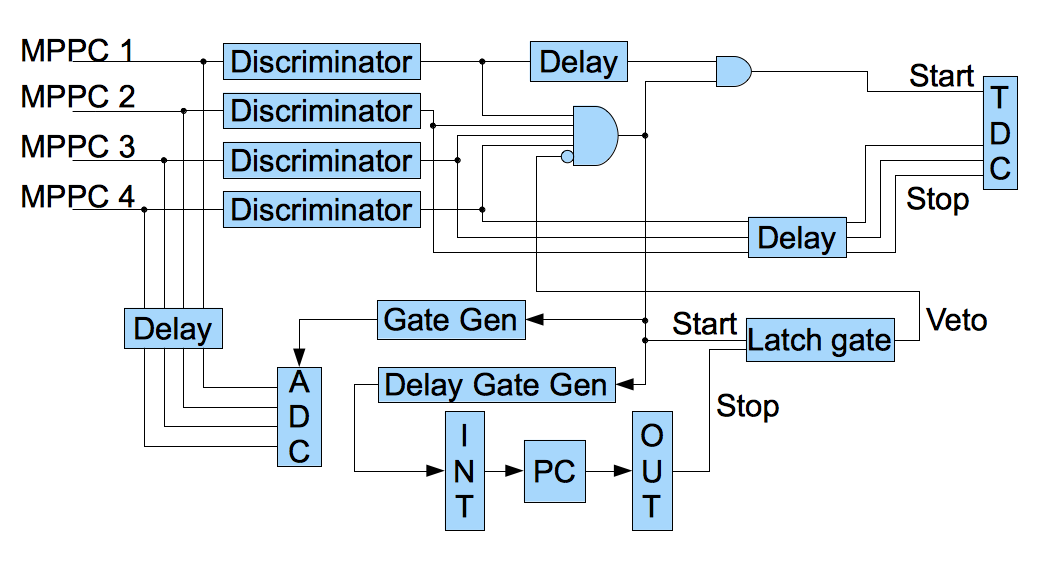
\includegraphics[width=.9\textwidth]{images/charged_flux/MuSIC1_DAQ_Block.png}
    \caption{Schematic of the DAQ used for measuring the charged particle flux. Horizontal blocks indicate NIM units whilst vertical ones were mounted in a CAMAC crate.}
    \label{fig:MuSIC1_DAQ_Block}
\end{figure}

To make the final measurement, the trigger rate, the majority of the DAQ was ignored and the four-fold co-incidence counted using a scaler. By counting the raw triggers affects of dead time could be negated and a truer value for the number of interactions obtained. For the 1D experiment measurements were made over 50~s with control done via hand, this obviously had limitations 

The positions of the two experiments are given in table~\ref{tab:charged_particle_positions} with respect to the centre of the beam-pipe.
\begin{table}
    \begin{center}
    \begin{tabular}{c|c|c|c|c|c}
        Measurement  &  \multicolumn{3}{c|}{Distance from centre of beam (cm)}         &  Scaler Time (s)  &  Readout \\
                     &    Horizontal    &       Vertical              &  Longitudinal  &                   &          \\
        \hline            
        1D           &  n/a             &  \(-5\), \(-15\), 0, 15, 5  &       6        &  50               & By-eye   \\
        2D           &  \(-17\), 0, 17  &  \(-16\), 0, 20, 25         &       85       &  20               & CAMAC    \\
    \end{tabular}
    \end{center}
    \caption{Positions at which the charged particle flux was measured, 1D refers to the first run in which only the vertical was measured, 2D refers to the second run in which horizontal measurements were also take. The distances from the beam-pipe were 6~cm for 1D measurements and 85~cm for 2D, this was due to mechanical constraints.}
    \label{tab:1d_res}
\end{table}

% section experimental_set_up (end) 
\section{Results} % (fold)
\label{sec:results}

The results from the measurements are presented in table~\ref{tab:1d_res}, for the 1D case, and table~\ref{tab:2d_res} in the 2D case. Errors on the rates are the square-root of the count and are propagated appropriately. The flux was calculated using:
\begin{align}
    j &= \frac{F(C - C_{off})}{I} \\
    I &= K(S - S_{off})
\end{align}
where \(j\) is the flux, \(F\) is a scaling factor, \(C\) is the trigger count with the beam on, \(C_{off}\) is the background trigger rate (i.e.\ with the beam off), \(S\) is the SEC count, \(S_{off}\) is the SEC count with the beam off and \(K\) is the SEC to current conversion factor. The scaling factor, \(F\), was  used in normalise runs with different conditions. For the 1D measurement there was a discrepancy between the first four and last 5 measurements due to damage to the MPPCs (one broke and another became detached from the scintillator). During the 2D measurements some of the runs were made with an upstream experiment in a different configuration; they changed stopping target from 5~mm of copper to 20~mm to magnesium for the last 3 runs.

\begin{table}
    \begin{center}
    \begin{tabular}{ c | r@{\( \pm \)}l | r@{\( \pm \)}l | r@{\( \pm \)}l | r@{\( \pm \)}l | r@{\( \pm \)}l | r@{\( \pm \)}l } 
        Height  &  \multicolumn{4}{c|}{Trigger Rate (kHz)}  
                                                             &  \multicolumn{4}{c|}{SEC (Hz)}  
                                                                            &  \multicolumn{2}{c|}{Factor}  
                                                                                        &  \multicolumn{2}{c}{Flux} \\
        (cm)   & \multicolumn{2}{c|}{Beam on}  
                                 & \multicolumn{2}{c|}{Beam off}  
                                           &  \multicolumn{2}{c|}{Beam on}  
                                                            &  \multicolumn{2}{c|}{Beam off}  &  \multicolumn{2}{c|}{ }  
                                                                                 &  \multicolumn{2}{c}{(kHz/A)} \\
        \hline
          0     &   43.0 & 6.1   &   \multirow{3}{*}{0.60} & \multirow{3}{*}{0.14}
                                           &    25.1 & 3.6   &   \multirow{3}{*}{7.6} & \multirow{3}{*}{1.1}
                                                                       &    \multirow{3}{*}{1.00} & \multirow{3}{*}{0.00}
                                                                                 &   72   & 19 \\
        \(-5\)  &   28.8 & 4.1   &    &    &    25.7 & 3.7   &    &    &    &    &   47   & 12 \\
        \(-15\) &   10.1 & 1.4   &    &    &    24.2 & 3.5   &    &    &    &    &   17.8 &  4.7 \\
        \hline
          5     &   33.3 & 4.7   &   \multirow{4}{*}{1.66} & \multirow{4}{*}{0.30}   
                                           &    26.0 & 3.7   &   \multirow{4}{*}{8.0} & \multirow{4}{*}{1.2}
                                                                             &    \multirow{4}{*}{1.65} & \multirow{5}{*}{0.33}
                                                                                        &   89   & 29 \\
          5     &   28.4 & 4.0   &    &    &    22.8 & 3.3   &   8.0 & 1.2   &     &    &   92   & 31 \\
         15     &   21.6 & 3.1   &    &    &    26.7 & 3.8   &   8.0 & 1.2   &     &    &   56   & 18 \\
         15     &   23.7 & 3.4   &    &    &    27.4 & 3.9   &   8.0 & 1.2   &     &    &   59   & 19 \\
         \hline
          0     &   26.1 & 3.7   &   0.68 & 0.15   &    26.0 & 3.7   &   8.1 & 1.2   &    1.65 & 0.33   &   71   & 23 \\
    \end{tabular}
    \end{center}
    \caption{Summary of the results from the measurement of the vertical charged particle flux. The rates were calculated with counts taken over 50~s, errors on the rates are the square root of the value. The `factor' column accounts for the fact that for the later measurements one MPPC was broken and another damaged, these measurements are then scaled by the ratio of two measurements at 0~cm. The error on the }
    \label{label}
\end{table}

 \begin{figure}[hptb]
    \centering
        \includegraphics[width=.9\textwidth]{images/charged_flux/hit_rate_rescaled.png}
    \caption{Results of the 1D measurements, the last 3 entries had damaged MPPCs as noted. These damaged points have had their values rescaled by the ratio of the two 0~cm values, one which had fully working MPPCs, the other was the last measurement.}
    \label{fig:images_hit_rate_rescaled}
 \end{figure}
 
 % TODO note re multiple computer measurements for trigger count
 \begin{table}
    \begin{center}
    \begin{tabular}{c|c|c|c|c|c|r@{\( \pm \)}l}
        % TODO Should these have errors? 
        X     &   Y    &  \multicolumn{2}{c|}{Trigger Rate (Hz)}  &  \multicolumn{2}{c|}{SEC (Hz)}  &  \multicolumn{2}{c}{Flux}     \\
        (mm)  &  (mm)  &  Beam On          &  Beam Off        &  Beam On    &  Beam Off    &  \multicolumn{2}{c}{(Hz/A)}   \\
        \hline % TODO Finish this!
          0  &    0    &   3438.1          &    5.3           &      51     &           9  & 54  &  4 \\
        -17  &   20    &   5897.4          &    5.3           &      51     &           9  & 93  &  7 \\
        -17  &  -16    &   1976.4          &    2.4           &      68     &           9  & 22  &  1 \\
        -17  &    0    &   4859.5          &    3.9           &      73     &           9  & 50  &  2 \\
         17  &    0    &   3158.0          &    4.5           &      76     &           9  & 31  &  1 \\
         17  &   20    &   5254.9          &    4.4           &      71     &           9  & 56  &  3 \\
         17  &  -16    &   1350.5          &    2.8           &      67     &           9  & 15  &  1 \\
          0  &  -16    &   2181.7          &    4.8           &      69     &           9  & 24  &  1 \\
          0  &   20    &   7126.8          &    3.6           &      64     &           9  & 86  &  5 \\
          0  &    0    &   3768.8          &    3.0           &      66     &           9  & 44  &  2 \\
          \hline
          0  &   25    &   2297.5          &    1.8           &      46     &           9  & 41  &  3 \\
        -17  &   25    &   3479.1          &    6.0           &      47     &           9  & 60  &  5 \\
          0  &   20    &   4004.4          &   11.9           &      60     &           9  & 52  &  3 \\
    \end{tabular}
    \end{center}
    \caption{Table of the results from the 2D measurement. Measurements were taken over 20~s using a CAMAC scaler.}
    \label{tab:2d_res}
 \end{table}
% section results (end)
\section{Analysis} % (fold)
\label{sec:analysis}

% section analysis (end)
% chapter charged_particle_flux (end)
\chapter{Muon Lifetime} % (fold)
\label{cha:muon_lifetime}
\section{Experimental Set Up} % (fold)
\label{sec:experimental_set_up}
% section experimental_set_up (end)
\section{Results} % (fold)
\label{sec:results}

% section results (end)
\section{Analysis} % (fold)
\label{sec:analysis}

% section analysis (end)
% chapter muon_lifetime (end)
\chapter{Momentum Spectrum} % (fold)
\label{cha:momentum_spectrum}
\section{Experimental Set Up} % (fold)
\label{sec:experimental_set_up}
% section experimental_set_up (end)
\section{Results} % (fold)
\label{sec:results}

% section results (end)
\section{Analysis} % (fold)
\label{sec:analysis}

% section analysis (end)

% chapter momentum_spectrum (end)


% part characterising_the_beam (end)


















% \part{Characterising the beam} % (fold)
% \label{prt:characterising_the_beam}
% % TODO: Measurements:: Measurements: Characterising the beam: write me
% \chapter{Introduction} % (fold)
% \label{sec:measurements_introduction}
% 
% Characterisation of the MuSIC beam was carried out over several years and through a number of experiments. Over the course of five beam-times three significant measurements were made to characterise the beam: the total charged particle flux, the muon lifetime and the momentum spectrum; table~\ref{tab:summary_music_beam_time} covers the details. Several other experiments were also carried out although these are not discussed here.
% \begin{table}[htpb]
%   \begin{center}
%   \begin{tabular}{c|c|c}
%     \multicolumn{2}{c|}{Dates}          & Measurements                                \\
%     Start            & Stop             &                                             \\
%     \hline                                                                             
%     29 July 2010     & 31 July 2010     & Charged particle flux.                      \\
%     13 February 2011 & 16 February 2011 & Muon lifetime in Cu and Mg.                 \\
%     19 July 2011     & 21 July 2011     & Muon yield (via lifetime).                  \\
%                      &                  & Muon yield (via muonic X-rays).             \\
%     22 October 2011  & 23 October 2011  & Neutron flux.                               \\
%     18 June 2012     & 22 June 2012     & Muon momentum spectrum (via lifetime).      \\
%                      &                  & Muon momentum spectrum (via muonic X-rays). \\
%   \end{tabular}
%   \end{center}
%   \caption{A summary of the five MuSIC beam-times with notes on the measurements made.}
%   \label{tab:summary_music_beam_time}
% \end{table}
% 
% \section{Experimental method} % (fold)
% \label{sec:experimental_method}
% All of the measurements discussed here use scintillators to measure the beam. As discussed in section~\ref{sec:charged_particle_interactions_in_matter} scintillators respond to ionisation by emitting photons. The number and spectrum of emitted photons depends on the amount of energy deposited and the characteristics of the material. A commonly quoted value for plastic scintillator's light yield is 1 photon per 100~eV of deposited energy~\cite{PDG particle detectors review}. 
% 
% To increase the proportion of light captured the scintillators were wrapped in mylar and then black-wrap. The combination of these two additional layers meant that any light exiting the scintillator would be reflected back in whilst external light was kept out to prevent background. The thickness of both the mylar and black-wrap were minimised in order to prevent excess energy loss in these layers.
% 
% Due to the large magnetic field present at the end of the beam large PMTs were not a viable option, instead a type of silicon photomultiplier (SiPM) called a `Multi-Photon Pixel Counter' (MPPC) was employed. Each MPPC is composed of an array of Avalanche Photodiodes (APD), an array typically contains between 100 and 1,600 individual APDs. An APD operates by maintaining a small region of doped silicon close to its breakdown voltage (for an MPPC this is \( \sim -\)70~V) when a photon is incident on this region an electron/hole pair is created via the photo-electric effect. The bias voltage is large enough to accelerate the electron/hole pair causing ionisation of the silicon and further pairs to be created. This `avalanche' of pairs has a gain of order \( 10^5 \), large enough (\( \sim \)25~mV) that with proper amplification and noise removal it can be detected.
% 
% The largest disadvantage to using MPPCs is that, due to their sensitivity, they're a noisy sensor. They typically have a false positive (the `dark count') rate of \( \mathcal{O}(150)\times10^3 \)~counts/s (cps). The dark count can be easily removed by rejecting low photon count events, a minimum voltage threshold of \( \sim 0.5\)~photo-electrons (p.e.) is used to measure the dark-count and, given the poisson-nature of the noise, a threshold of 1.5~p.e. will remove the majority of dark counts (\(\gtrsim60\%\)). 
% 
% % TODO Good example of MPPC signal
% 
% In order to make the actual measurements first the signals from the MPPCs had to be processed and then digitised. The exact details of this varied from measurement to measurement (and are discussed in the relevant chapters) the general process was always the same: first the signal is amplified, then it is determined if the signal is to be measured (triggering) and finally the signal is read out. 
% 
% Amplification of the signals was done to change the signal to one which was above the threshold of the discriminator units. The discriminator units normally had a minimum threshold of 10~mV with a minimum \emph{viable} (i.e.\ stable) threshold of \( \sim \)50~mv; the signals from an MPPC are generally \( \mathcal{O}(10) \)~mV obviously too small for the discriminators, even before any attenuation. In order to make the MPPC signals detectable the signal was amplified twice: first in the experimental hall and again at the DAQ-station, downstairs. 
% 
% Once the MPPC signal has been amplified suitably it is converted to a digital signal using a discriminator. The advantage of converting the analogue MPPC signal to a digital one is that the digital signal is much easier to manipulate and process, unfortunately there is a loss of information which has to be accounted for. Digitisation is done using a discriminator which is a device that receives an analogue input and sends a digital output. The digital output is sent (`asserted') when the input exceeds some pre-set threshold. Assuming that the input exceeds the discriminator's threshold for long enough to be detected (normally \(\gtrsim8\)~ns) the output will be asserted for as long as the input is or the pre-set minimum output width; which ever is longer. 
% 
% Whilst the MPPCs are all similar they are not identical so to account for variance in gain and inaccuracies in the analogue amplification discriminator thresholds were normalised to the number of photo-electrons that any particular voltage corresponded to. Setting the threshold was done using an oscilloscope to visualise the impact of any particular threshold by using the discriminator's output as the oscilloscope's trigger whilst plotting the analogue signal trace, an example of this can be seen in figure~\ref{fig:set_dis_thrs_for_mppc}.
% 
% \begin{figure}[hptb]
%   \centering  
%     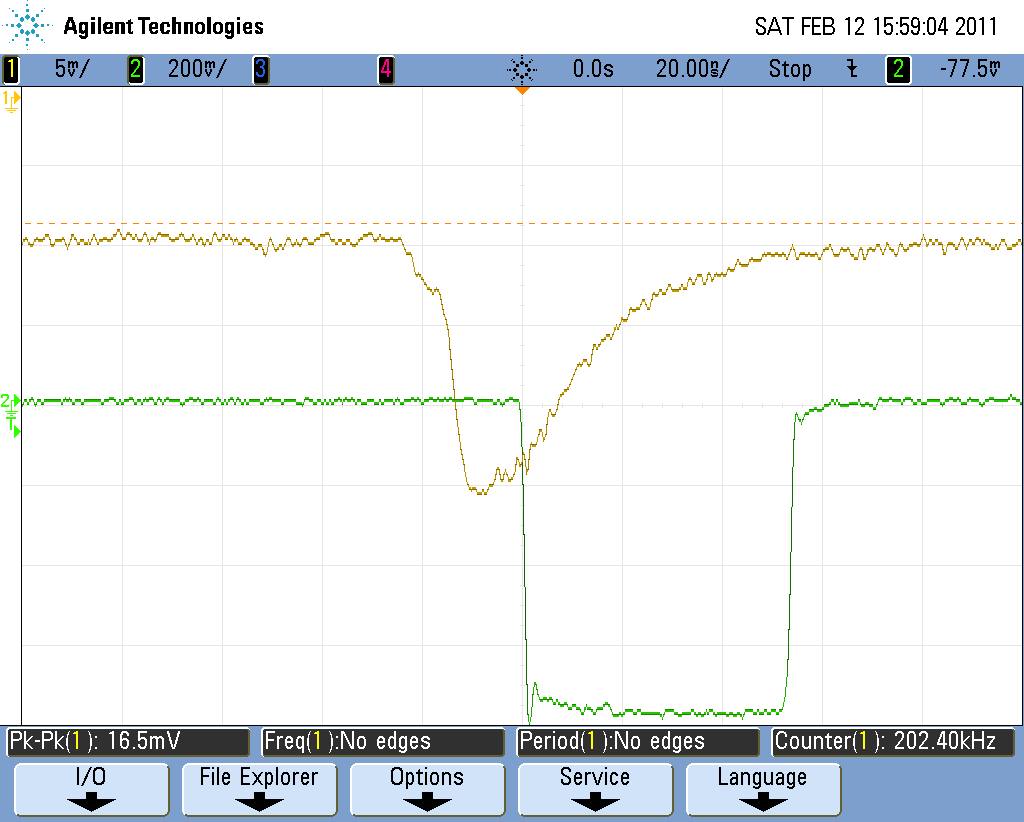
\includegraphics[width=.9\textwidth]{images/edit/scope_dis_ch_2.png}
%   \caption{An example oscilloscope trace being used to set the discriminator threshold. In this case the threshold is set to \( \sim \)1.5~p.e. (i.e.\ \( \sim- \)15~mV). The discriminator signal being used to trigger is shown in green whilst the input MPPC signal is brown. There are 200~mV/div for the discriminator signal whilst the MPPC signal has 5~mV/div; the time resolution is 20~ns/div.}
%   \label{fig:set_dis_thrs_for_mppc}
% \end{figure}
% 
% Careful setting of the discriminator threshold removes the majority of noise from the signal it doesn't remove all of it, to account for this a more stringent requirement is placed upon signals from the MPPC: co-incidence across MPPCs. Whilst it's entirely possible for a burst of noise to mimic a signal of several photo-electrons in one MPPC it is highly unlikely for this to occur in more than one MPPC. The standard second stage of the DAQ is to require that all the MPPCs on a scintillator register a suitably strong (e.g.\ at least \( >1.5\)~p.e.) signal. The co-incidence requirement is also combined with any additional logic for the system, e.g.\ busy signals from the readout computer or anti-co-incidence with other scintillators. 
% 
% % TODO Calculate 
% 
% Anti-co-incidence is used heavily in the muon lifetime measurements. All the muons produced at MuSIC are travelling at a reasonable fraction of the speed of light, this means that scintillators with a suitably small separation (\( \mathcal{O}(10)\)~mm) will detect such a muons almost simultaneously. By placing a high density `stopping target' between two such scintillators it is possible to detect which muons have likely stopped by looking for a hit in the upstream scintillator and no corresponding hit in the downstream scintillator. 
% 
% % TODO probably want to split this into separate subsections, one per measurement device e.g. scaler, (PH)ADC and (MH)TDC as well as information on the modules used and CAMAC/NIM in general
% 
% As well as discrimination of the MPPC signals there are three other useful measurements to be made: counting the number of signals from the discriminator, measurement of the size of the MPPC signals and measurement of the timing difference between up and downstream scintillators (if used). Whilst the discriminator is a measurement of the signal size it has a very low information content, by using an Analogue to Digital Converter (ADC) it is possible to get a much more precise measurement of the either the peak potential (so called `Peak Height' or PH-ADC) of the signal or the integrated charge. For MPPCs the peak value of the potential is the most useful number so it is this that we measure. When two scintillators are used by measuring the time differences between an anti-co-incident hit in the upstream scintillator (and only the up-stream scintillator) and then subsequent hits in the downstream scintillator (after a suitable anti-co-incidence or veto window) it's possible to reconstruct the lifetime of the upstream particle, for this to work a Multi-Hit Time to Digital Converter (MH-TDC) is used. A MH-TDC is required as some number of the downstream hits will be noise (often electrons) the noise appears as a flat background whilst the signal, electrons produced in the decay of the upstream muon, are correlated with the start time through an exponential. 
% 
% % TODO figure out what SEC stands for
% % TODO Add info on SEC proton current measurement
% % TODO How well do we know the energy of the initial proton beam, especially at low energies? 
% % TODO need info on why 380 MeV is pion production threshold
% As well as measuring the properties of the muon beam in order to make reasonable measurements we need to understand the properties of the initial proton beam. The key value is the proton beam's current which defines the number of protons at the PCS and hence its efficiency. The proton beam's current is estimated during operation using a Secondary Emission Chamber (SEC). The SEC contains a thin gold foil that is connected to an ammeter enabling direct measurement of a fraction of the beam during a run. The exact fraction absorbed by the gold foil is determined during a calibration run in which the entire beam's current is measured using a copper block to absorb it.
% 
% % section experimental_method (end)
% %%%%%%%%%%%%%%%%%%%%%%%%%%%%%%%%%%%%%%%%%%%%%%%%%%%
% 
% % chapter measurements_introduction (end)
% %%%%%%%%%%%%%%%%%%%%%%%%%%%%%%%%%%%%%%%%%%%%%%%%%%%
% \chapter{Charged Particle Flux} % (fold)
% \label{sec:charged_particle_flux}
% % TODO: Measurements:: Charged Particle Flux: write me
% % TODO: Measurements:: Charged Particle Flux: cover scint design
% % TODO: Measurements:: Charged Particle Flux: cover DAQ
% % TODO: Measurements:: Charged Particle Flux: cover what happened
% % TODO: Measurements:: Charged Particle Flux: Check dimensions & positions of 1D scint
% % TODO: Measurements:: Charged Particle Flux: Check dimensions & positions of 2D scint
% Two measurements of the charged particle flux were made: the first using a long strip of scintillator (380\(\times\)30\(\times\)10~mm) positioned across the face of the beam pipe at a variety of heights; the second measurement was made using a \(35\)~mm radius \( 20 \)~mm deep disk. 
% 
% Both measurements were made using a scaler to count the raw trigger rate, which was recorded with the beam both on and off. The raw trigger rate is defined as a signal from all MPPCs that passes discrimination. To normalise the trigger rate between runs the proton beam intensity was measured using SEC.
% 
% % TODO check distance from beampipe
% The vertical measurements were made \( 50 \)~mm from the end of the MTS at: \( -15 \), \( -5 \), \( 0 \), \( +5 \) and \( +15 \)~mm, measured from the centre of the beam-pipe. For each position both the SEC and trigger rate were measured with the beam on, and then to measure the bias measured off. Each value was measured for 50~s.
% 
% % To make the measurement to values were recorded: the total trigger rate (i.e.\ the number of charged particles) and the intensity (i.e.\ current) of the proton beam (for normalisation). A trigger was defined as an all-MPPC co-incidence above the discriminator threshold. Measurement of the pro
% \begin{figure}[hptb]
%   \centering
%     \includegraphics[width=.9\textwidth]{images/hit_rate_rescaled.png}
%   \caption{Charged particle flux at a variety of vertical positions, 50~cm from the end of the MTS, at MuSIC. The note below each point indicates when the data was taken, the three right-most points have been rescaled (using the ratio of the 0~mm values) to account for the broken MPPCs (as noted). Measurement was taken using a \( 380\times30\times8 \)~mm scintillator mounted on aluminium support struts.}
%   \label{fig:1D_hit_rate_rescaled}
% \end{figure}
% 
% \begin{figure}[hptb]
%   \centering
%     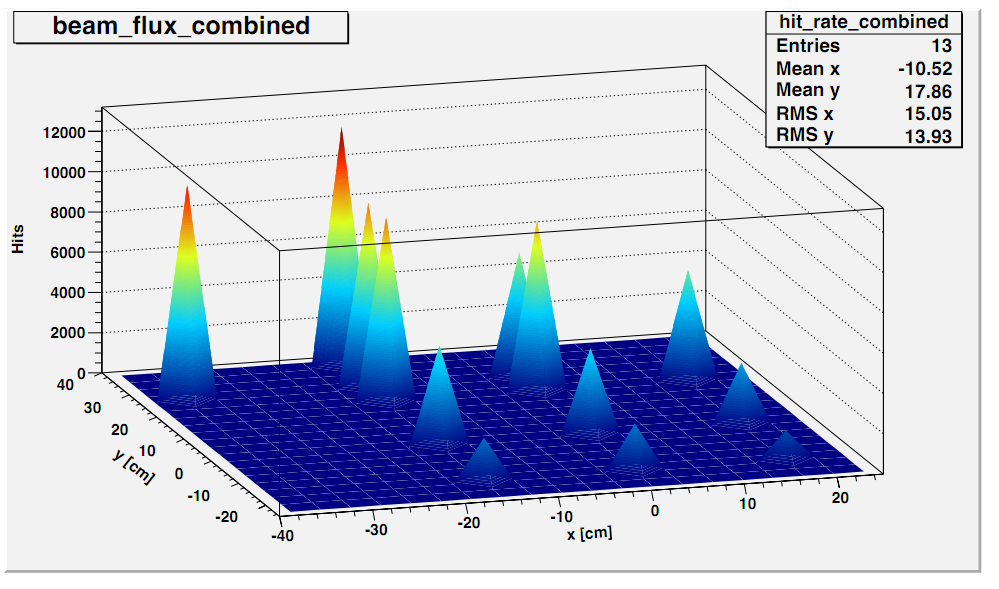
\includegraphics[width=.9\textwidth]{images/2D_hit_rate_dist.png}
%   \caption{The charged particle flux at 5~cm from the end of the beam-pipe, measured using a 7~cm diameter scintillator.}
%   \label{fig:2D_hit_rate_dist}
% \end{figure}
% 
% %%%%%%%%%%%%%%%%%%%%%%%%%%%%%%%%%%%%%%%%%%%%%%%%%%%%%%%%%%%%%%%%%%%%%%%%%%%%%%%%%%%
% 
% % TODO experimental methods dicussion of ADC
% % TODO experimental methods dicussion of TDC
% % TODO experimental methods dicussion of Scaler
% % TODO experimental methods dicussion of SEC
% 
% Measurements of the charged particle flux were made during the first two beam times. The first was carried out using a \( 380\times30\times10\)~mm scintillator bar mounted at a variety of heights whilst the second was done using a \( 20\times35 \)~mm disk that could be moved on both the horizontal and vertical axises. During each measurement ADC and TDC data was taken but ultimately was not used in analysis. The core measurement were scaler readings of the total trigger rate and SEC measurements of the proton beam used to normalise the data.
% 
% The first measurements were taken at 6~cm from the beam-pipe with the second at 85~cm. The DAQ used was similar for each: two stages of amplification followed by the discriminator set to 1~p.e.\ the discriminator was fed to a co-incidence detector that created a gate for ADC readout. TDC readings were taken to measure the time difference in each MPPC triggering. A schematic of the set up can be seen in figure
% % TODO DAQ block diagram
% 
% To measure the particle flux the total trigger rate for each scintillator was measured for 50~s; at the same time the SEC was also measured. The beam would then be switched off to measure the same values for background results. The total charged particle flux was then calculated using 
% \begin{equation} \label{eq:particle_rate}
%   \text{Rate} = \frac{C_{\text{On}} - C_{\text{Off}}} {K(I_{\text{On}} - I_{\text{Off}})}
% \end{equation}
% Where \( C \) is the trigger count, \( K \) is the SEC to Ampere conversion factor and \( I \) is the proton current as determined by SEC. 
% 
% \section{Vertical charged particle flux} % (fold)
% \label{sec:vertical_charged_particle_flux}
% As has been noted the vertical charged particle flux was measured using a scintillator bar, read out was done using four S10362-11-050U Hamamatsu MPPC mounted on the bar's ends as shown in figure~\ref{fig:1D scint}. The scintillator was supported on two aluminum structs and held in place using cable ties. 
% 
% Severn measurements were made at five heights, 
% \begin{table}
%   \begin{center}
%   \begin{tabular}{ c | c | c | c | c | c | c} 
%       Height & \multicolumn{2}{c|}{Trigger Count}   & \multicolumn{2}{c|}{SEC}  &  Particle Flux & Adjusted Flux \\
%       (cm)   & Beam on            & Beam off        &  Beam on  &  Beam off   &  (Hz/A)          & (Hz/A) \\
%       \hline
%       0      &  2,151,736  &  \multirow {4}{*}{30}  &  1,255  &  \multirow {4}{*}{381}  &  2,461.91  & n/a  \\
%       -5     &  1,438,685  &                        &  1,286  &                         &  1,589.67  & n/a  \\
%       -15    &    446,302  &                        &  1,212  &                         &  537.03    & n/a  \\
%       -15    &    502,596  &                        &  1,208  &                         &  607.70    & n/a  \\
%       \hline
%       5      &  1,663,702  &  \multirow {4}{*}{83}  &  1,298  &  \multirow {4}{*}{398}  &  1,848.47  & 2,957.39  \\
%       5      &  1,420,836  &                        &  1,142  &                         &  1,909.61  & 1,783.28  \\
%       15     &  1,080,170  &                        &  1,336  &                         &  1,151.48  & 1,886.07  \\
%       15     &  1,185,051  &                        &  1,371  &                         &  1,217.85  & 2,264.10  \\
%       0      &  1,307,015  &  34                    &  1,298  &  404                    &  1,461.95  & 2,957.39  \\
%   \end{tabular}
%   \end{center}
%   \caption{Summary of the results from the measurement of the vertical charged particle flux. The measurements above the line were taken with all four MPPCs still functioning whilst those below only had three fully functioning MPPCs, to reflect the impact this had the flux is adjusted by the ratio of the two measurements made at 0~cm.}
%   \label{label}
% \end{table}
% 
% % TODO charged particle flux: Schematic of the 1D scintillator with MPPC mounting
% % section vertical_charged_particle_flux (end)
% % chapter charged_particle_flux (end)
% %%%%%%%%%%%%%%%%%%%%%%%%%%%%%%%%%%%%%%%%%%%%%%%%%%%
% \chapter{Muon Lifetime} % (fold)
% \label{sec:muon_lifetime}
% % TODO: Measurements:: Muon Lifetime: write me
% % TODO: Measurements:: Muon Lifetime: cover set up
% % TODO: Measurements:: Muon Lifetime: cover daq
% % TODO: Measurements:: Muon Lifetime: cover first data set vs second
% \begin{figure}[hptb]
%   \centering
%     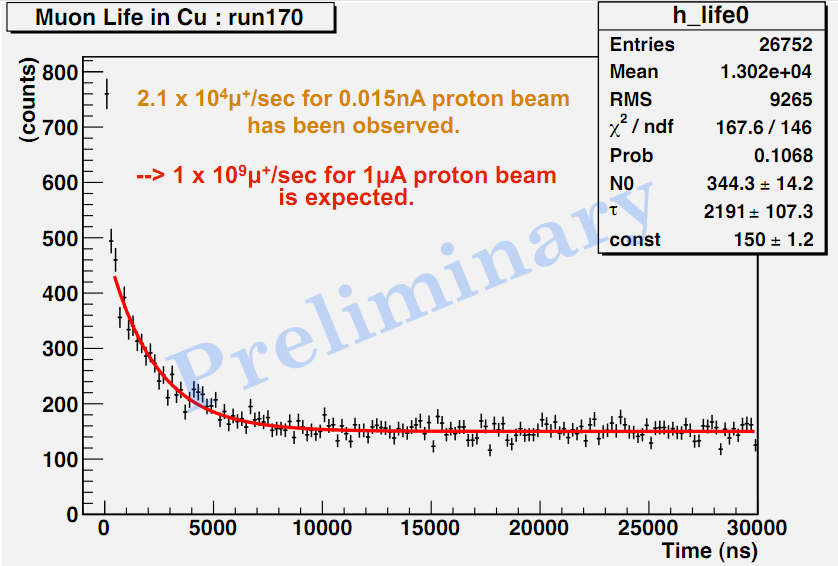
\includegraphics[width=.9\textwidth]{images/muon_decay_feb.png}
%     % TODO Add PDG muon lifetime
%   \caption{First measurement of the muon lifetime at MuSIC. A single exponential is used for the fit and the lifetime measured is compatible with the global measurement (PDG MUON LIFETIME~\cite{pdg for muons}).  } 
%   \label{fig:3_measurements_images_muon_decay_feb}
% \end{figure}
% 
% \begin{figure}[hptb]
%   \centering
%     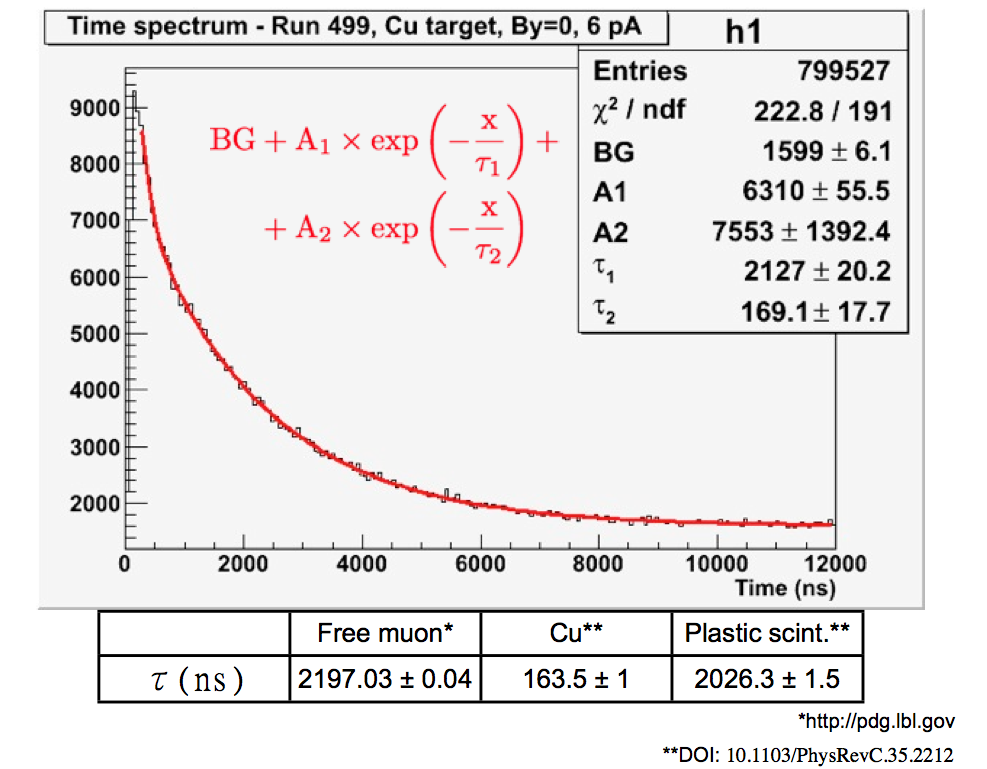
\includegraphics[width=.9\textwidth]{images/muon_decay.png}
%   \caption{Second measurement of muon lifetime at MuSIC, made 19\( ^{th} \)--21\( ^{st} \)~July~2011. With the improved statistics a double exponential was used allowing an estimation of the \( \mu^{-} \) component to be made. This estimation is made by looking for muons stopping in the copper target. The muon lifetime is low but this is to be expected as there is a hidden component due to negative muons interacting with the scintillator and air~\cite{Muon lifetime in scintillator}.}
%   \label{fig:3_measurements_images_muon_decay}
% \end{figure}
% 
% 
% % chapter muon_lifetime (end)
% %%%%%%%%%%%%%%%%%%%%%%%%%%%%%%%%%%%%%%%%%%%%%%%%%%%
% \chapter{Muon Momentum Spectrum} % (fold)
% \label{sec:muon_momentum_spectrum}
% % TODO: Measurements:: Muon Momentum Spectrum: write me
% % TODO: Measurements:: Muon Momentum Spectrum: daq & set up 
% % TODO: Measurements:: Muon Momentum Spectrum: noise
% % TODO: Measurements:: Muon Momentum Spectrum: sensitve to
% % TODO: Measurements:: Muon Momentum Spectrum: stopping targets
% 
% \section{Experimental Set Up} % (fold)
% \label{sec:experimental_set_up}
% To measure the momentum distribution of the muon beam two separate problems had to be solved: firstly how to count the muons produced and secondly how to determine their momentum. The first problem is addressed by looking for muon decays through timing data whilst the second is dealt with by using degraders and a thin stopping target to select specific momentums. 
% 
% \subsection{Detector} % (fold)
% \label{sub:detector}
% The detector consisted of an aluminium degrader who's thickness could be varied to select different momentum ranges, a thin (0.5~mm) upstream counter and a thicker (3.5~mm) downstream counter on either side of a 0.5~mm copper stopping target. A schematic of the detector can be seen in figure~\ref{fig:setup}. Based on simulation (section~\ref{sec:simulated_data}) we can predict the mean momentum of muons that decay for different degrader thicknesses, the momentum distributions for the muons that stop can be seen in figure~\ref{fig:stopped_muon_mom} whilst the initial muon momentum distribution is given in figure~\ref{fig:initial_muon_momentum}, the mean momentums are also tabulated in table~\ref{tab:stopped_muon_mom}.
% \begin{figure}[htbp]
%     \centering
%         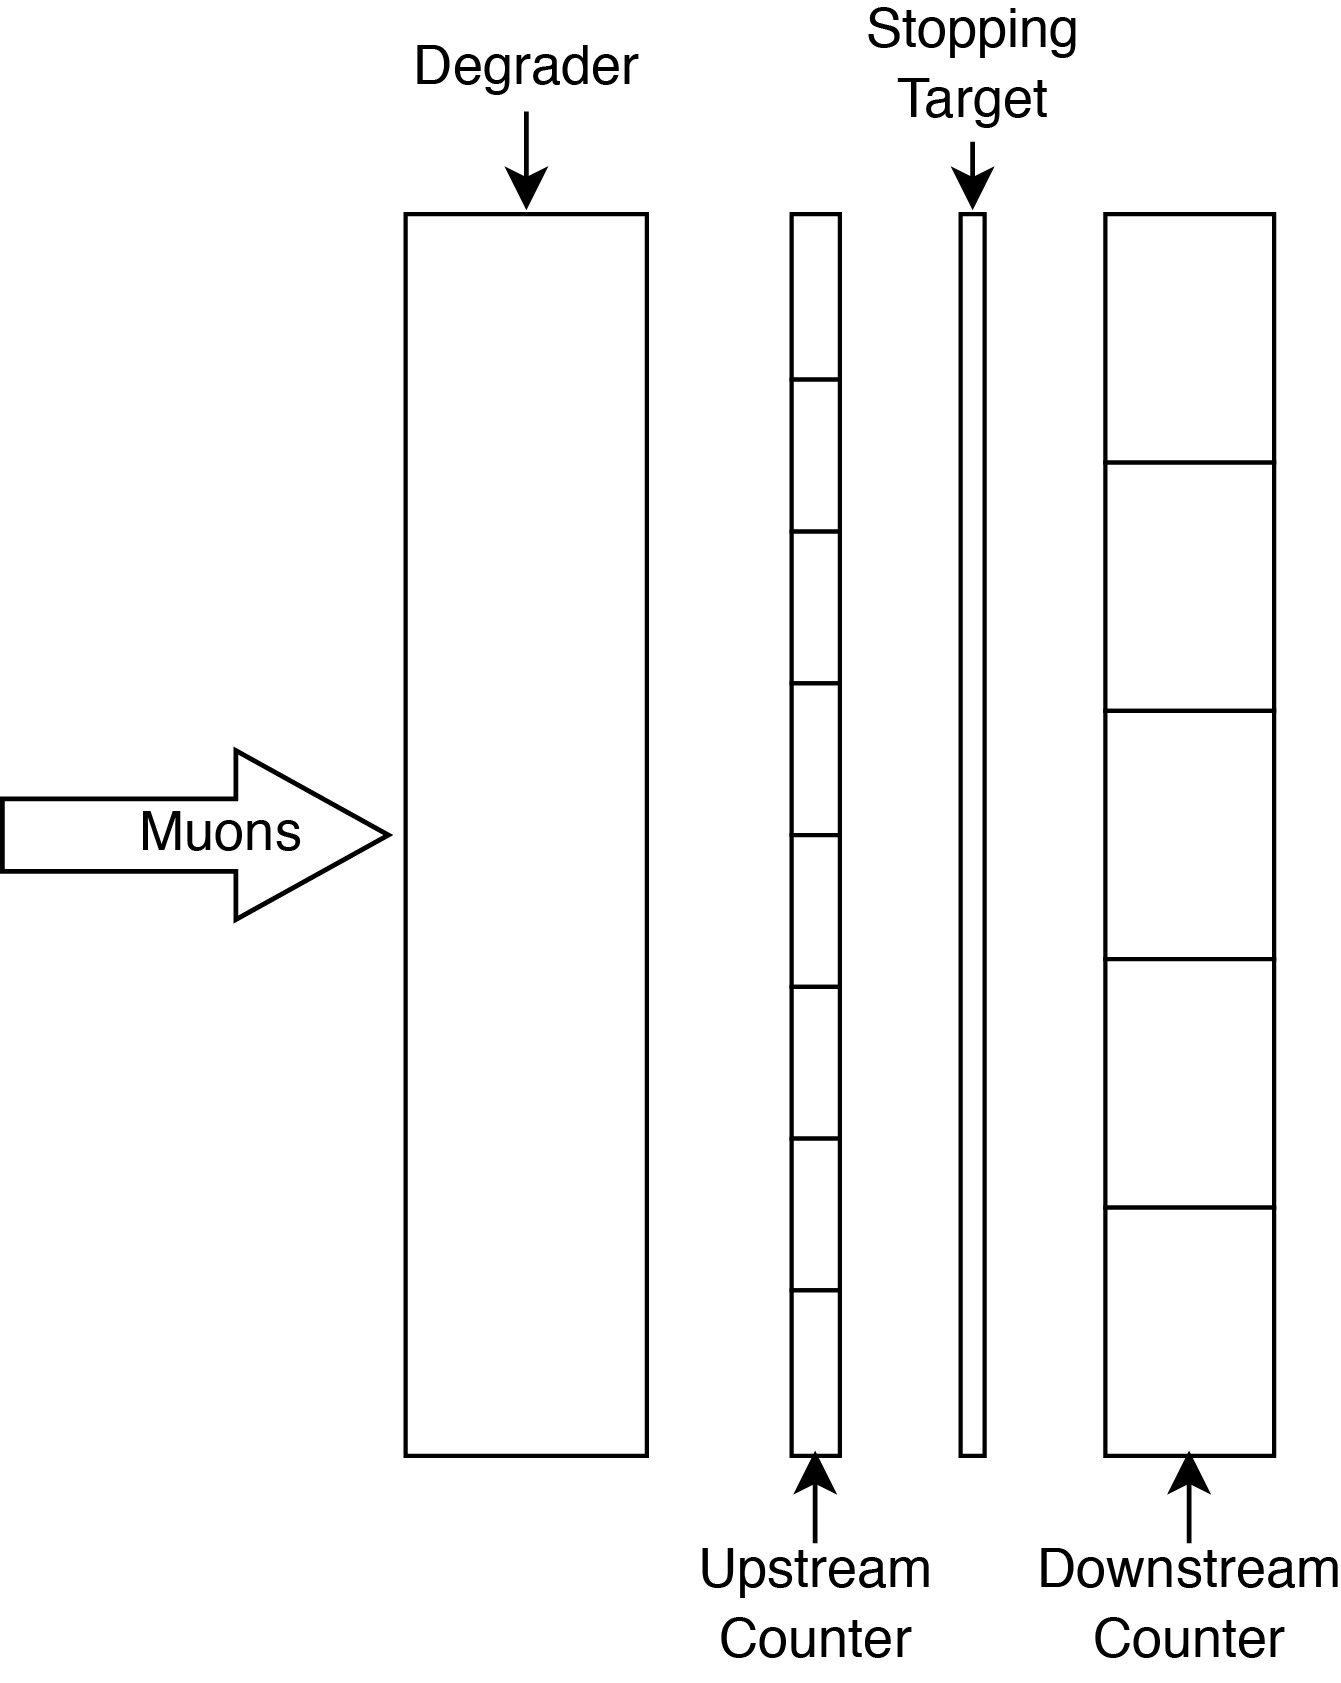
\includegraphics[scale=0.5]{images/Detector_setup.png}
%     \caption{Experimental set up of the detector for MuSIC~5 (not to scale)}
%     \label{fig:setup}
% \end{figure}  
% %
% \begin{figure}[htbp]
%     \centering
%         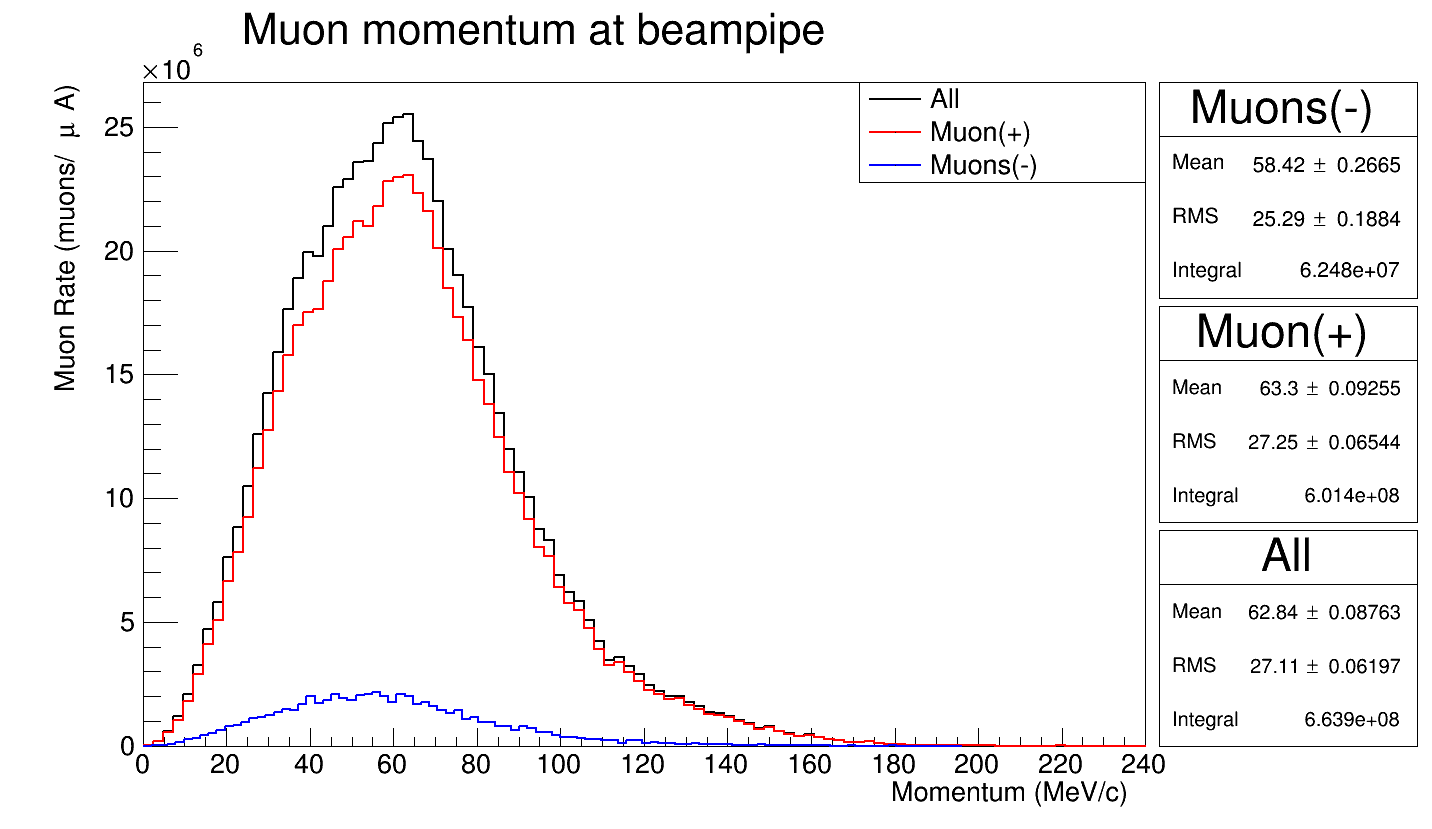
\includegraphics[width=\textwidth]{images/muon_momentum_at_beam_pipe_exit.png}
%     \caption{The initial muon momentum at the exit of the beampipe as simulated by G4Beamline~\cite{G4BL} (G4BL). The muon rate has been normalised to \( 1\mu \)A of proton current which is the maximum available at the RCNP. Section~\ref{sub:g4bl_particle_production} for further details of the G4BL simulation.}
%     \label{fig:initial_muon_momentum}
% \end{figure}
% %
% \begin{figure}[htbp]
%     \centering
%         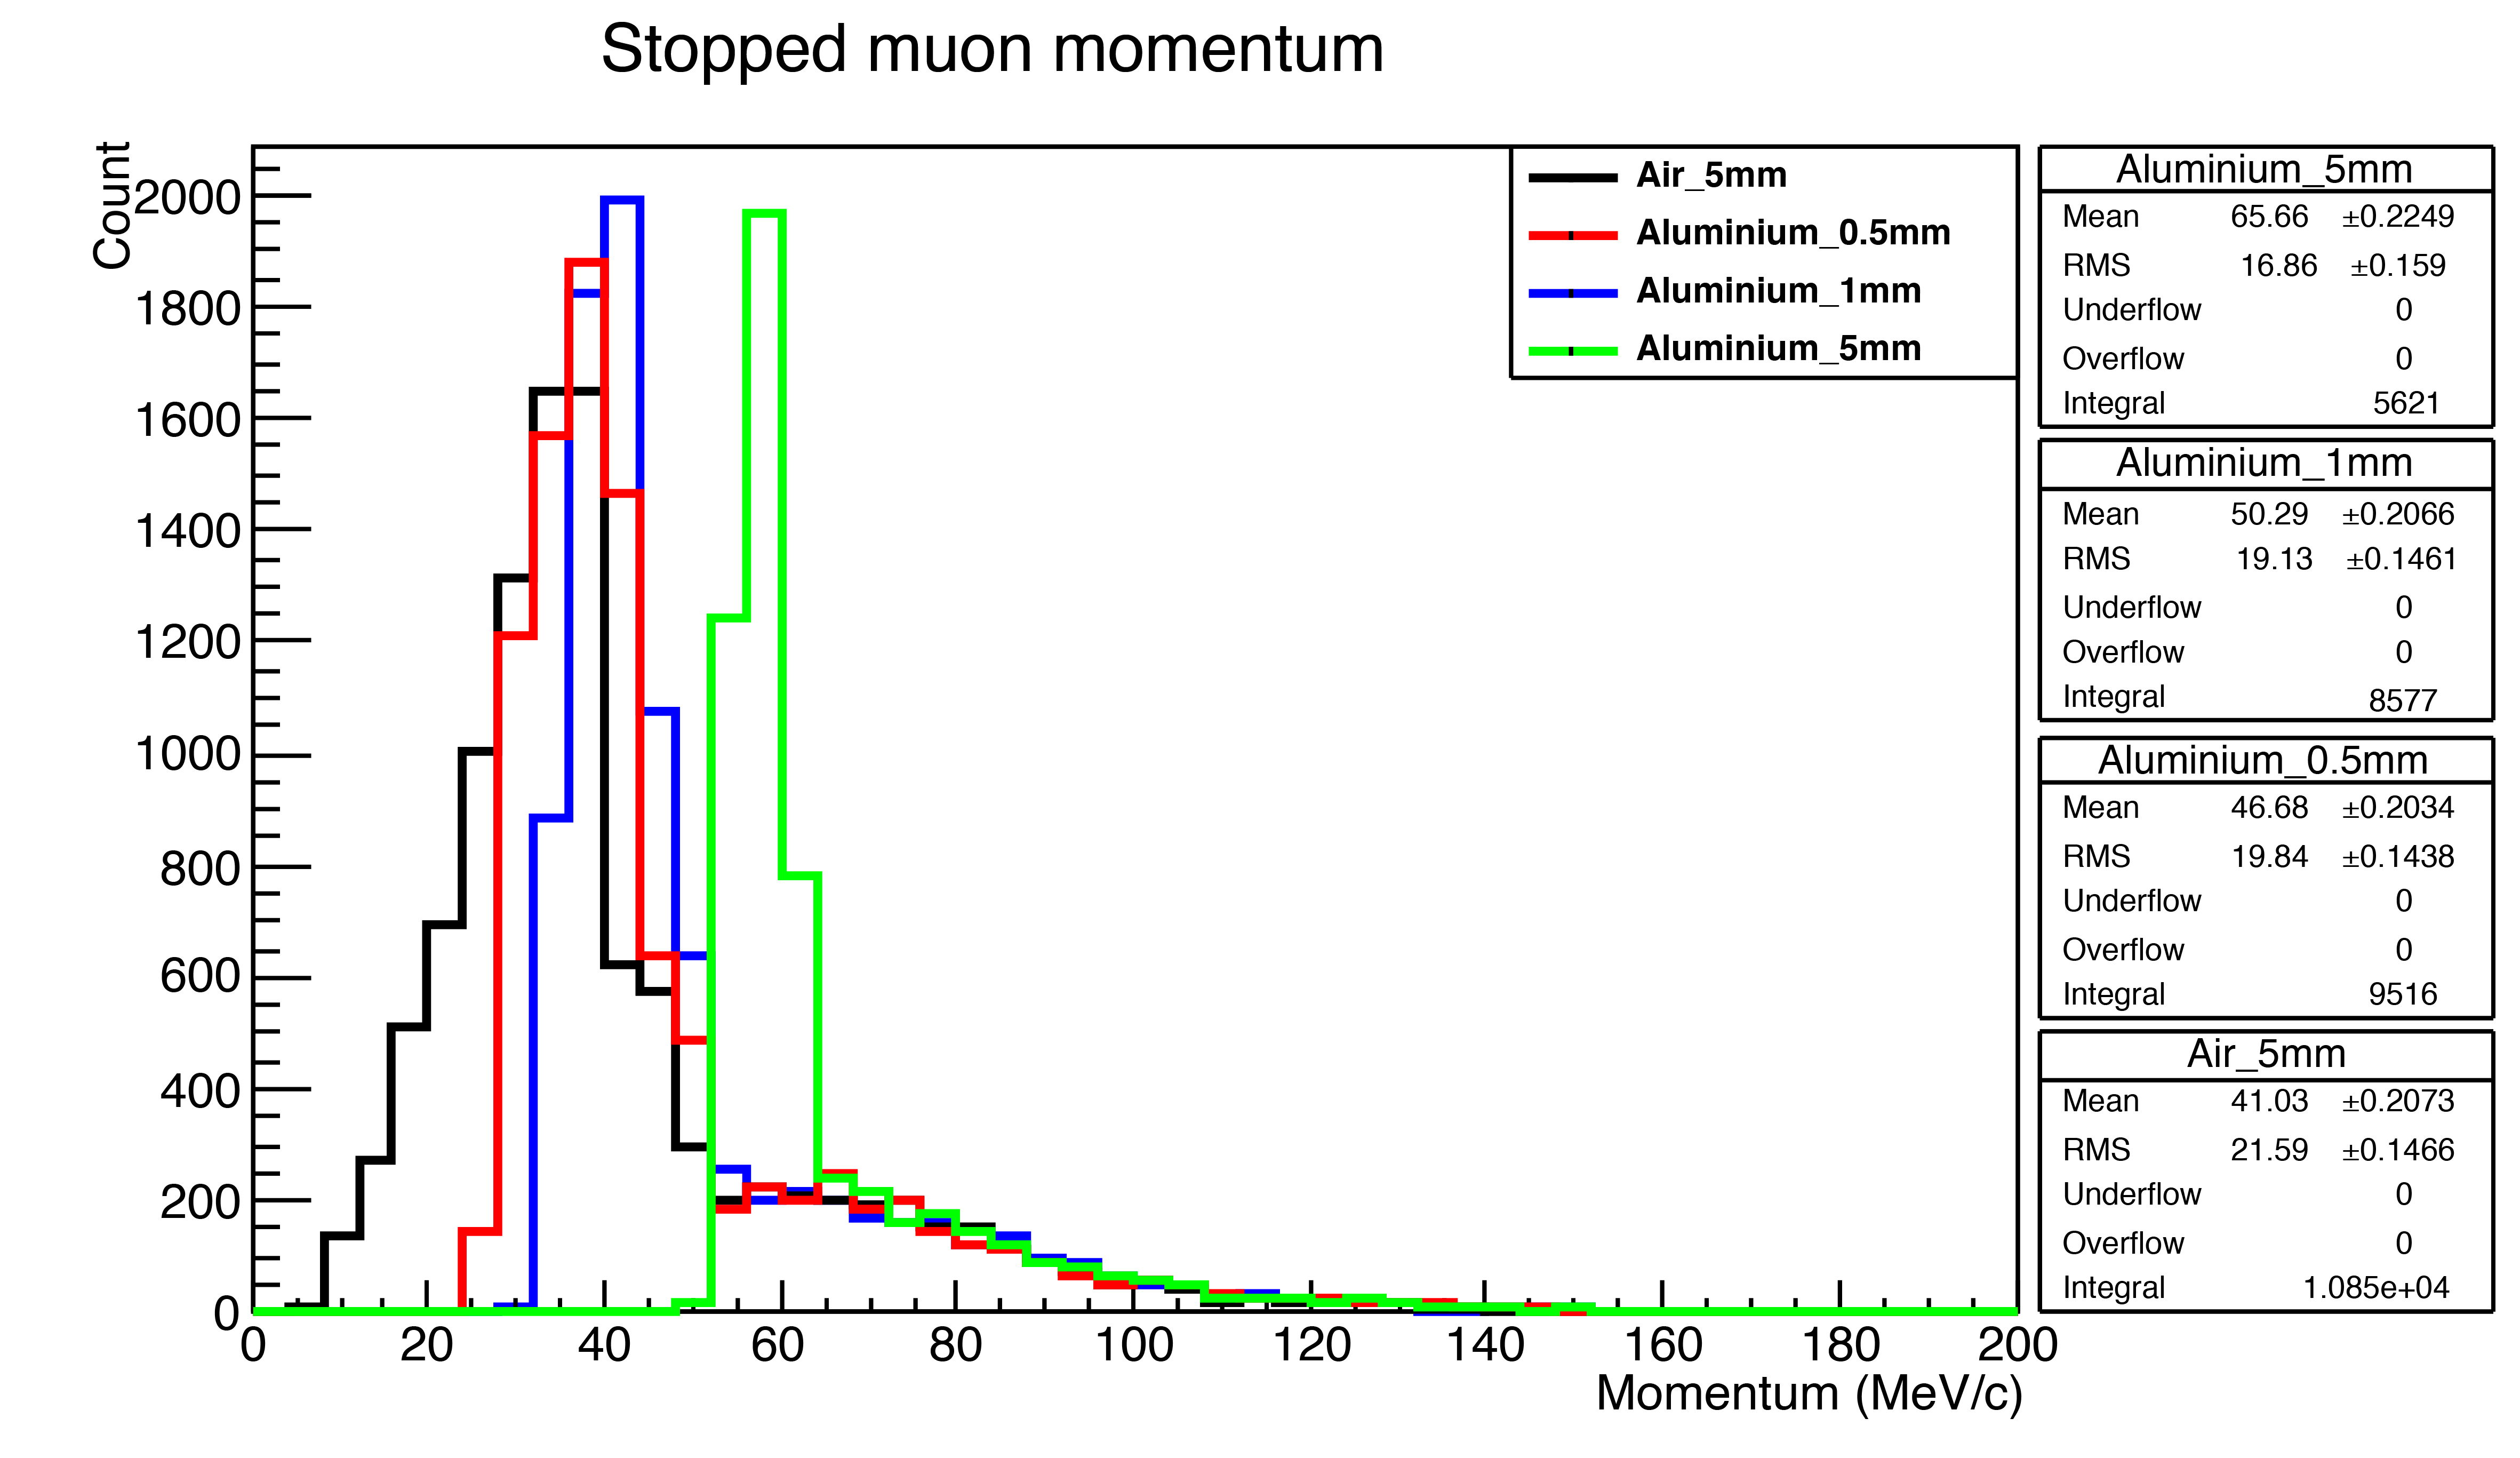
\includegraphics[width=\textwidth]{images/stopped_muon_momentum.png}
%     \caption{Simulated momentum distributions for muons that decay between the up and downstream counters. 900~M initial protons were simulated with a range of aluminium degrader thicknesses. Stopped muons were those seen in the upstream counter that subsequently had a daughter electron seen in the downstream counter. This plot shows raw counts for the 900~M initial protons.}
%     \label{fig:stopped_muon_mom}
% \end{figure}
% %
% \begin{table}
%     \begin{center}
%     \begin{tabular}{r|r@{ $\pm$ }l|r@{ $\pm$ }l} % r@{ $\pm$ }l should align on \pm
%         Degrader (mm) & \multicolumn{2}{|c|}{Mean (MeV/c)} & \multicolumn{2}{|c}{RMS (MeV/c)}\\
%         \hline
%         Air 5.0       & 41.03 & 0.21 & 21.59 & 0.15 \\
%         Aluminium 0.5 & 46.68 & 0.20 & 19.84 & 0.14 \\
%         Aluminium 1.0 & 50.29 & 0.21 & 19.13 & 0.15 \\
%         Aluminium 5.0 & 65.66 & 0.22 & 16.86 & 0.16 \\
%     \end{tabular}
%     \end{center}
%     \caption{Simulated mean momentums for decaying muons. 900~M initial protons}
%     \label{tab:stopped_muon_mom}
% \end{table}
% %
% The counters used were mylar wrapped scintillators with read-out performed by MPPCs mounted on either end of a wave length shifting fibre bounded along the long axis of the scintillator using optical cement. The signals from each pair of MPPCs are combined and amplified before being passed to the data acquisition system (DAQ) for processing.
% 
% % subsection detector (end)
% \subsection{Data Acquisition} % (fold)
% \label{sub:data_acquisition}
% The Data Acquisition (DAQ) took two measurements: the time at which signals arrived from the MPPC and the strength of those signals. The timing measurements are of the primary concern for this analysis. The DAQ itself had 3 distinct stages: discrimination, trigger formation and readout.
% 
% MPPCs are inherently noisy devices and discrimination is required to separate signal due to scintillation events from the MPPC's noise. A voltage threshold was set which (when exceeded) created a digital signal. Two thresholds were used: a lower one for the upstream counter and a higher one for the downstream counter. The lower threshold for the, thinner, upstream counters enabled better detection of minimally ionising muons whilst the higher downstream threshold enabled better detection of the more ionising electrons produced by muon decay. 
% 
% Using the signals from the discriminator a trigger was created based on the signature of muonic decay: the anti-coincidence of the up and downstream counters. It was assumed that a muon that doesn't decay in the detector region will be seen in both counters within a very small window of time ($<$50~ns). The only other constraint on the formation of a trigger was that the system wasn't busy in which case the trigger couldn't be accepted.
% 
% The trigger, once formed, signalled the start of readout. There were 3 modules to be read out via VMEbus (VME): a charge to Digital Converter (QDC), a scaler and a Multi-hit Time to Digital Converter (MTDC) which is of primary concern for this analysis. The MTDC recorded all signals  within a 20\mus{} period following the trigger that passed discrimination and that were anti-coincident with the other counter. Using a MTDC ensured that even if some beam remnant or dark event created a signal then the real signal would also be recorded and determined with background removal. The channel assignment used for the MTDC can be seen in table~\ref{tab:mtdc_ch}. To increase the accuracy of the MTDC the trigger time is recorded on a seperate channel called `TDC0'.
% \begin{table}
%     \begin{center}
%     \begin{tabular}{c|c|c}
%         Channel & Signal & Notes\\
%         \hline
%         0  & TDC0 & Time at which the trigger was formed \\
%         \hline
%         1  & U1   & \multirow{8}{*}{Upstream Counter}\\
%         2  & U2   & \\
%         3  & U3   & \\
%         4  & U4   & \\
%         5  & U5   & \\
%         6  & U6   & \\
%         7  & U7   & \\
%         8  & U8   & \\
%         \hline
%         9  & D1   & \multirow{5}{*}{Downstream counter}\\
%         10 & D2   & \\
%         11 & D3   & \\
%         12 & D4   & \\
%         13 & D5   & \\
%         \hline
%         14 & Ge1  & \multirow{2}{*}{Germanium counter (not used in this analysis)}\\
%         15 & Ge2  & \\
%     \end{tabular}
%     \end{center}
%     \caption{Channel assignment for the MTDC. QDC channel assignment follows the same scheme but has no entry for channel 0 (as TDC 0 will be one of the upstream counters by design).}
%     \label{tab:mtdc_ch}
% \end{table}
% 
% The scaler was used to record system diagnostics (e.g. the trigger rate) by polling the scaler regularly during each run. The QDC recorded the strength of the trigging signal by integrating its charge over 100~ns. This information has not be incorporated into the current analysis but may be used in later analysis, for example to apply more stringent energy cuts at trigger time or for selection of regions of interest. The QDC had the same channel assignment as the TDC but without the germanium detector (as it had its own analogue to digital converter) and TDC0 (which was a digital signal).
% \begin{table}
%     \centering
%     \begin{tabular}{c|c|l}
%         Channel & Signal & Notes\\
%         \hline
%         0 & SEC & Measure of the proton current\\
%         1 & Trigger & number of t0's\\
%         2 & U and $\overline{\text{D}}$ & count of potential triggers\\
%         3 & U & Upstream only\\
%         4 & D & Downstream only\\
%         5 & Scint & -\\
%         6 & unused & -\\
%         7 & clk & Record of time passed\\
%     \end{tabular}
%     \caption{Table of scaler channels and their designation}
%     \label{tab:scaler_chs}
% \end{table}
% \section{Run Data} % (fold)
% \label{sec:run_data}
% As figure~\ref{fig:analysis_flow_diagrm} shows there are 5 stages in preparing the experimental data for analysis (receipt of the data from MIDAS, de-serialisation, calibration, restructuring and histogramming). These will will be explained in more detail in the following sub-sections but the general process will be discussed here. The first stage is the receipt of data from the DAQ via MIDAS, this creates files of raw data which has to be de-serialised in the next stage before having calibration applied to it. The final stages are to restructure the data according to channel and then create histograms of the TDC values ready for analysis. 
% 
% These processes are split across 4 programs: MIDAS; mu\_analysis and mid2root\_converter (which act on .root and .mid MIDAS files respectively); and finally tdc\_file.py which is a python script for creating the TDC histograms.
% 
% For the analysis 6 runs were chosen, all using the 0.5~mm copper stopping target. For 5 of the runs an aluminium degrader was used. The run information is summarised in table~\ref{tab:run_summary}.
% \begin{table}
%   \begin{center}
%   \begin{tabular}{c|c|c|c}
%       Run ID & Time (sec) & Current (nA) & Degrader (mm) \\
%       \hline
%       448    & 9,221      & 1.534E-02    & 0.0   \\
%       451    & 1,001      & 1.546E-02    & 0.5   \\
%       452    & 4,924      & 1.313E-02    & 0.5   \\
%       455    & 6,307      & 1.332E-02    & 1.0   \\
%       458    & 5,144      & 1.363E-02    & 5.0   \\
%       459    & 2,452      & 1.238E-02    & 5.0   \\
%   \end{tabular}
%   \end{center}
%   \caption{Summary of the runs selected for this analysis. The degrader used aluminium and the stopping target 0.5~mm copper.}
%   \label{tab:run_summary}
% \end{table} 
% \subsection{Data from MIDAS} % (fold)
% \label{sub:data_from_midas}
% MIDAS is `a general purpose data acquisition system for small and medium scale experiments'~\cite{ritt2012midas} and is the primary interface to the DAQ via VME. 
% 
% MIDAS stored the raw data from each run as a single file either in its own binary xml format (.mid files) or in ROOT~\cite{Brun199781} format (.root). Data was read from the VME crate in two asynchronous modes: `Trigger' and `Scaler' each corresponded to a separate tree structure in the resulting file. The majority of the time the system operated in trigger-mode: whenever a trigger was formed the controlling PC was informed and once the data had been gathered readout of the MTDC and QDC occurred via the VME. Scaler mode occurred at regular intervals and consisted of reading the diagnostics data gathered by the scaler, this did not reset the module which continued to accumulate data. 
% 
% Each tree contained a branch per module being read, the trigger tree also had also branch for errors (named `ERR'). The branches all had the same structure: an integer that recorded the number of values read and an array of integers containing those values. For the scaler and QDC modules the number of values read out was the same for every trigger as both had a fixed number of channels and took one measurement on each. The MTDC had a variable number of values to read out as it could record multiple hits on each channel.
% % subsubsection data_from_midas (end)
% \subsection{De-Serialisation} % (fold)
% \label{sub:de_serialisation}
% The first raw data from MIDAS for the MTDC and QDC were serialised and mangled with the channel number this means that they require processing before the real values can be extracted. Below are brief summaries of the algorithms used to de-serialise the MTDC data (listing~\ref{lst:mtdc_algo}), for full listings, including de-serialisation methods for QDC, see appendix~\ref{app:deserialisation}.
% %
% \begin{listing}[htbp]
%     \begin{minted}[gobble=4]{c++}
%     tdc_value      =  raw_val & 0x001f ffff
%     tdc_channel    = (raw_val & 0x03e0 0000) >> 21
%     tdc_valid_read = (raw_val & 0xf800 0000) == 0x0
%     \end{minted}
%     \caption{Method for de-serialising CAEN V1290N~\cite{CAENV1290N} data}
%     \label{lst:mtdc_algo}
% \end{listing}
% % subsection de_serialisation (end)
% \subsection{Calibration} % (fold)
% \label{sub:calibration}
% The MTDC has a stated least significant bit resolution of $\sim$25~ps with a 21 bits of data per value, this gives a maximum value of 52\mus{}. Conversion from the stored value to real, trigger aligned, time is done using the formula:
% \begin{align}\label{equ:tdc_calibration}
%     t'   &= 0.024414(t - \text{TDC}0)
% \end{align}
% where $t'$ is the calibrated time, $t$ is the de-serialised MTDC value and TDC$0$ is the de-serialised trigger time. The value $0.024414$ is the calibration co-efficient as determined in Tran Nam's work~\cite{timecalibNam2012}
% % subsection calibration (end)
% \subsection{Restructure} % (fold)
% \label{sub:restructure}
% In order for the MIDAS data to be easily manipulated it was restructured. The initial format was a simple structure of one branch for each module (i.e. one for MTDC one for the QDC and a final one for errors). A second tree was used to store the scaler values. Each branch had a leaf for the number of values and a leaf with the array of values.
% 
% In the restructured file each channel is a branch of a tree with the following leaves: QDC, TDC0, nHITS, TDC[nHITS]. The QDC value is self-explanatory, TDC0 was the trigger time, nHITS was the number of entries recorded by the MTDC for that channel and TDC was an array of the values. The error data was ignored as was the scaler tree as these can be read from the original file if needed and neither was required for de-serialisation or calibration.
% % subsection restructure (end)
% \subsection{Histogramming} % (fold)
% \label{sub:Histogramming}
% Once the data has been restructured it is trivial to create a histogram of the TDC data for each channel which forms the basis of the later analysis. A basic bin width of 1~ns was used and a range from 0 to 20\mus. A time of 0 was used for the lowest bin as, although the data window began at 50~ns, the MTDC recorded data as a sliding window so some values prior to the trigger were also recorded. All the histograms for (i.e. for all channels for all runs) were saved in the same root file.
% % subsection histogramming (end)
% % section run_data (end)
% %%%%%%%%%%%%%%%%%%%%%%%%%%%%%%%%%%%%%%%%%%%%%%%%%%%%%%%%%%%%%%%%%%%%%%%%%%%%%%
% \section{Secondary calculations} % (fold)
% \label{sec:secondary_calculations}
% There are two secondary calculations that need to be performed to calculate the muon yield. These are the acceptance, the fraction of the total beam we can expect to detect, and the dead time, a measure of how much of the time the detector is unable to process new data due to being busy.
% \subsection{Acceptance} % (fold)
% \label{sub:acceptance}
% To calculate the acceptance the ratio of initial muons to muons that passed a `trigger' cut was calculated. This is done by counting the number of muons in simulated G4BL output (section~\ref{sub:g4bl_particle_production}) and then using a macro similar to that used to digitise the simulation output (section~\ref{sub:digitisation_histogramming}) to mimic the triggering process.
% 
% The main difference between the acceptance macro (appendix~\ref{appsub:acceptance}) and the digitisation macro (appendix~\ref{appsub:digitisation_macro}) were in the cuts applied to select the particles. Rather than any possible parent particle in the upstream detector only muons are selected, similarly, in the downstream detector only electrons who had a parent muon are selected. A final requirement is that the time difference between muon and electron is greater than 50~ns.
% 
% The acceptance is then the ratio of muon/electron pairs to the initial number of muons:
% \begin{align}
%     \text{Acceptance} &= \frac{\text{Decay muons}}{\text{Initial Muons}} \label{equ:acceptance}
% \end{align}
% It is worth noting that given the above definition and method the acceptance changes due to the thickness and type of degrader used. Obviously a degrader that removed the majority of the muons from the beam will have a smaller acceptance as a smaller fraction of the beam will have survived to be detected. The results of the acceptance calculations are given in table~\ref{tab:acceptance}, the macro used can be seen in appendix~\ref{appsub:acceptance}.
% \begin{table}
%     \begin{center}
%     \begin{tabular}{c| r@{ $\pm$ }l | r@{ $\pm$ }l | r@{ $\pm$ }l | r@{ $\pm$ }l }
%         Degrader (mm) & \multicolumn{2}{|c}{Count (no cut)} &
%                         \multicolumn{2}{|c}{Count ($\Delta t>50$~ns)} &
%                         \multicolumn{2}{|c}{Initial Muons} &
%                         \multicolumn{2}{|c}{Acceptance (\%)}\\
%         \hline
%               Air 5.0 & 6330 & 80 & 4540 & 67.4 & 95719 & 309.4 & 4.7 & 0.1\\
%         Aluminium 0.5 & 5636 & 75 & 3999 & 63.2 & 95719 & 309.4 & 4.2 & 0.1\\
%         Aluminium 1.0 & 5222 & 72 & 3689 & 60.7 & 95719 & 309.4 & 3.9 & 0.1\\
%         Aluminium 5.0 & 3632 & 60 & 2472 & 49.7 & 95719 & 309.4 & 2.6 & 0.1\\
%         
%     \end{tabular}
%     \end{center}
%     \caption{The variance of acceptance with degrader thickness. In the final acceptance a cut on $\Delta t$ requiring it to be $>$50~ns was used to account for the anti-coincidence of the downstream counter. The number of initial muons is from the G4Beamline simulation.}
%     \label{tab:acceptance}
% \end{table}
% % subsection acceptance (end)
% \subsection{Dead time} % (fold)
% \label{sub:dead_time}
% The calculation of the dead time is unlike that of the acceptance as it was calculated based on the real data rather than simulation. Using the scaler it is possible to estimate how much of the time the DAQ was busy and hence what percentage of data was missed. 
% 
% As was stated in section~\ref{sub:data_acquisition} the scaler was used to record diagnostics on the DAQ. To calculate the dead time only two are needed, the trigger count and the potential trigger count which can be used to calculate the dead time thus:
% \begin{align}
%     D = \frac{\text{Potential Triggers}}{\text{Good Triggers}}
% \end{align}
% Where potential triggers are considered any anti-coincidence of the up without the downstream counter and a good trigger is one in which this occurs without the system being busy. The results for are given in table~\ref{tab:dead_time}. Obviously, the dead time is not used in the yield calculations using the simulated data.
% \begin{table}
%     \begin{center}
%     \begin{tabular}{c|c|c|r@{ $\pm$ }l|r@{ $\pm$ }l|r@{ $\pm$ }l }
%         Run & Degrader (mm of Al) & Run time (s) &
%                               \multicolumn{2}{|c}{Good Triggers} &      
%                               \multicolumn{2}{|c}{Potential Triggers} &
%                               \multicolumn{2}{|c}{Dead time (\%)} \\
%         \hline
%         448 & 0.0 & 9221 & 9652965 & 3106 & 15678757 & 3959 & 61.57 & 0.03 \\
%         451 & 0.5 & 1001 &  767321 & 875  &  1070366 & 1034 & 71.69 & 0.11 \\
%         452 & 0.5 & 4944 & 3459886 & 1860 &  4667767 & 2160 & 74.12 & 0.05 \\
%         455 & 1.0 & 6307 & 4090246 & 2022 &  5372409 & 2317 & 76.13 & 0.05 \\
%         458 & 5.0 & 5144 & 2049077 & 1431 &  2454952 & 1566 & 83.47 & 0.08 \\
%         459 & 5.0 & 2452 &  915314 & 956  &  1077534 & 1038 & 84.95 & 0.12 \\
%     \end{tabular}
%     \end{center}
%     \caption{Dead time for each run along with the number of potential and good triggers. Run time is included to show the origin of the different counts.}
%     \label{tab:dead_time}
% \end{table}
% % subsection dead_time (end)
% \subsection{Gain stability} % (fold)
% \label{sub:gain_stability}
% In order to better understand possible sources of systematics in the experiment the total trigger rate for each run was plotted over time. The gain stability should then be proportional to this trigger rate, giving a measure of how well the detector was working and highlighting any possible problems in the run. To plot this value the events produced in a run were divided into 10 sections, each containing an equal number of events. Using the values recorded by the scaler the length of each section in seconds could be determined (channel 7, see table~\ref{tab:scaler_chs}) as could the number of triggers seen in that section (channel 1). The results are plotted in figure~\ref{fig:gain_stability}, note that as the degrader thickness is increased the fit value decreases which is consistent with fewer particles reaching the detector. Full listings for plotting the gain stability can be found in appendix~\ref{appsub:gain_stability}.
% %
% \begin{figure}[htbp]
%     \centering
%         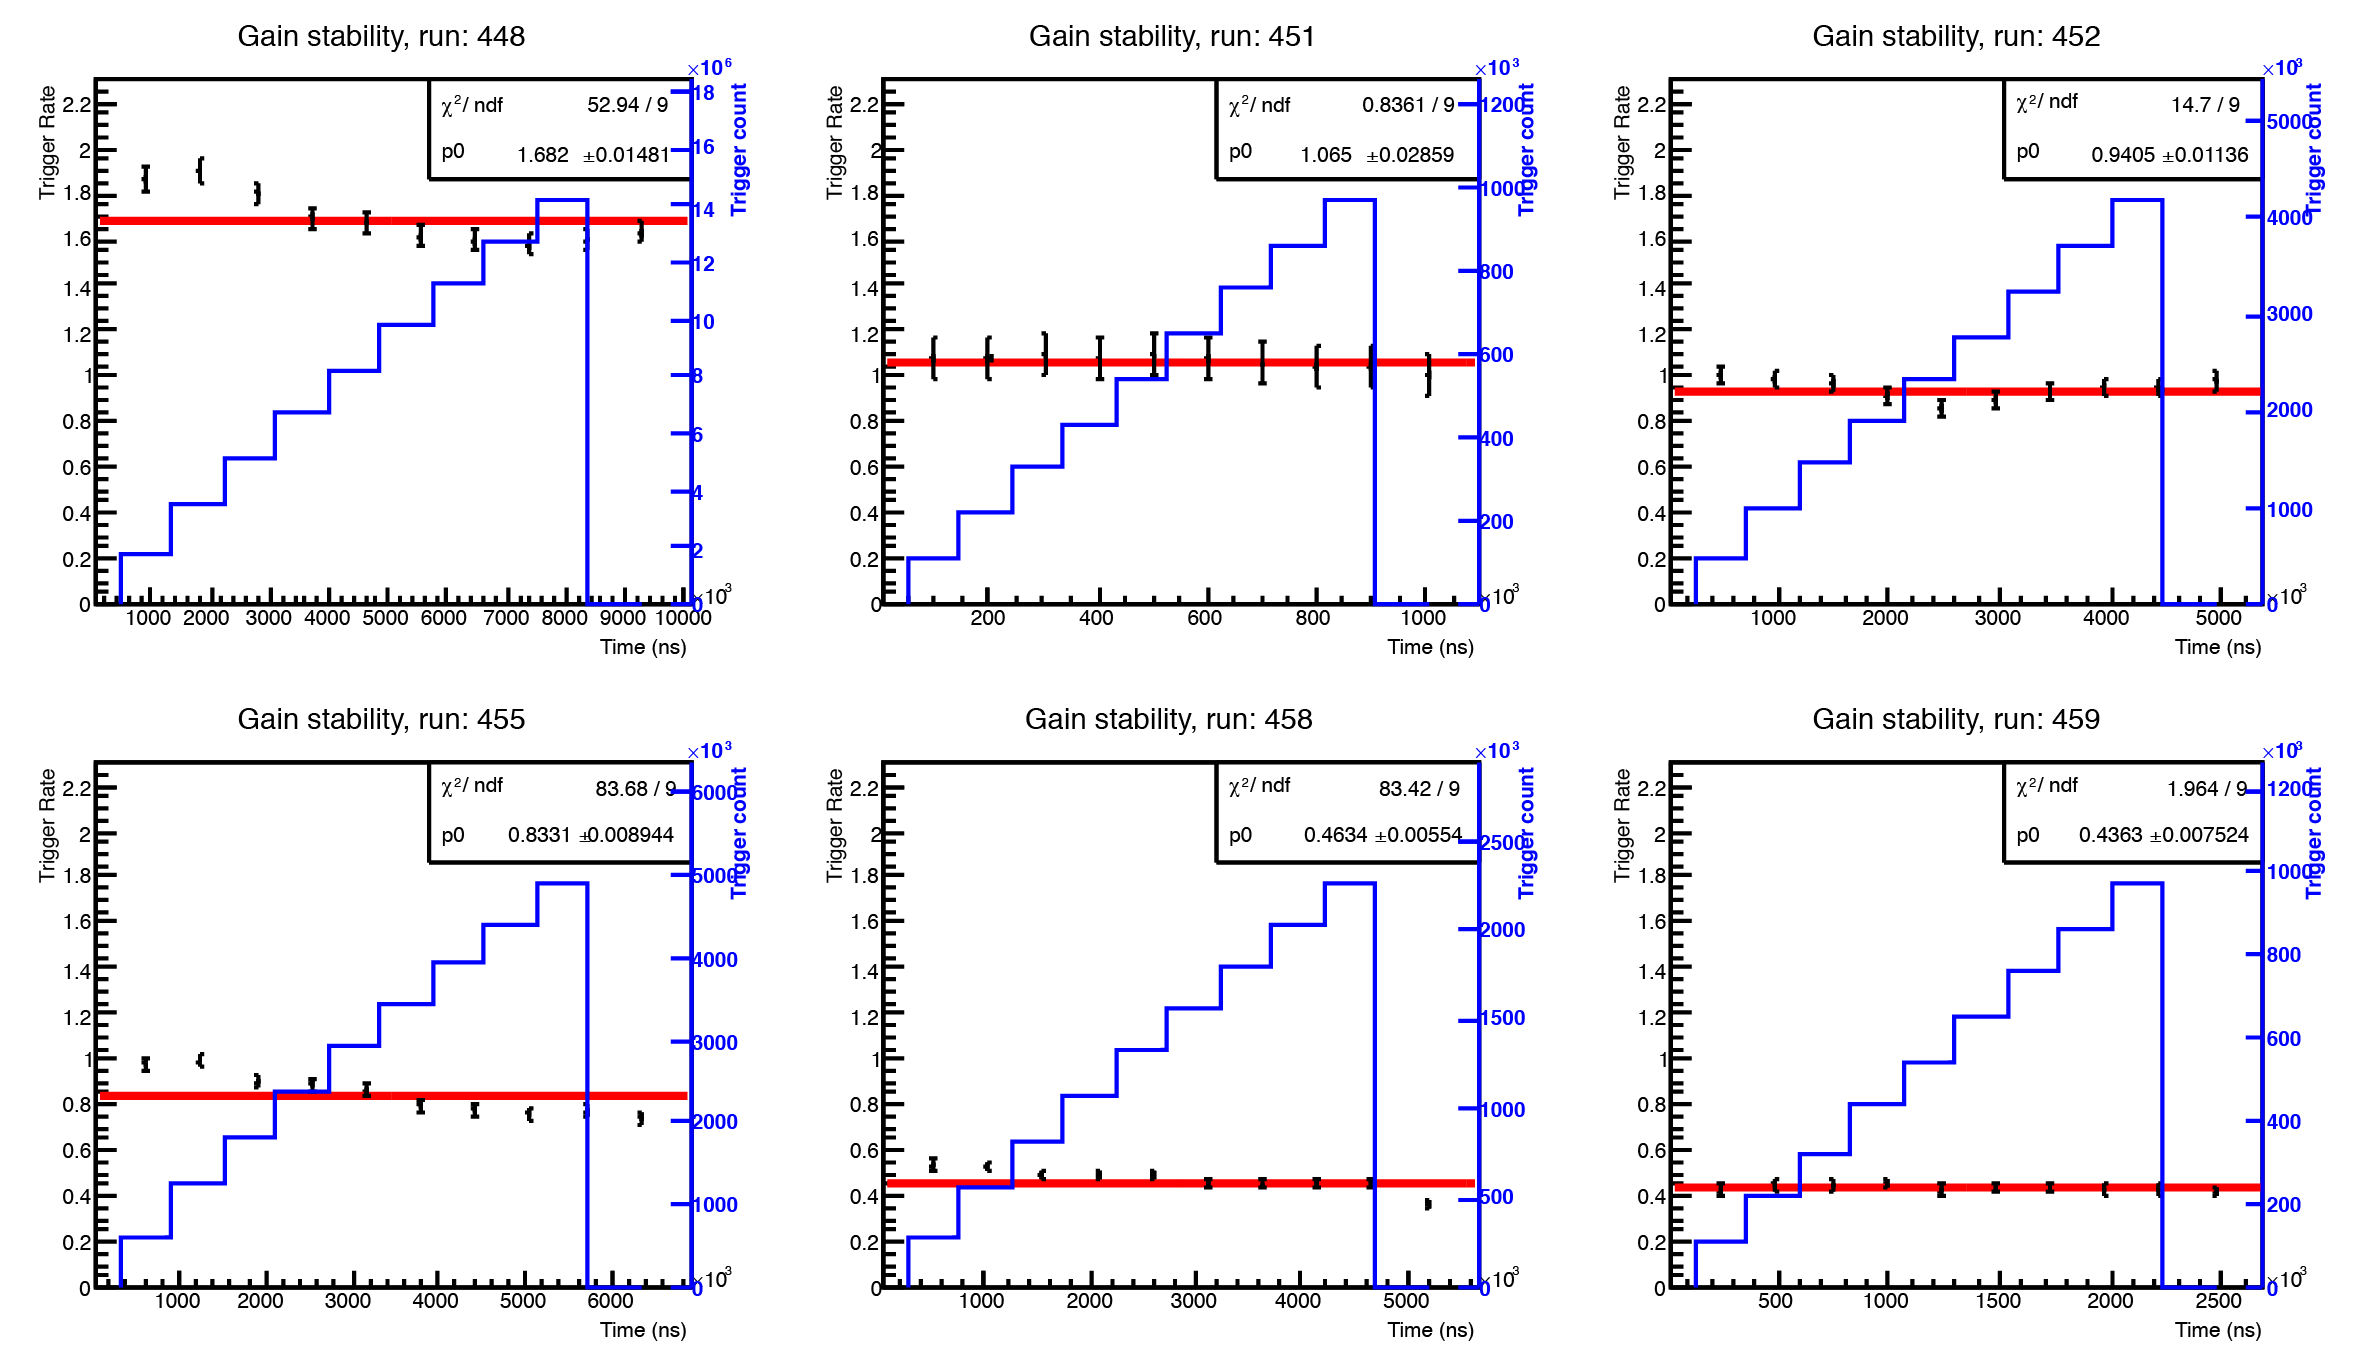
\includegraphics[width=\textwidth]{images/gain_stability.png}
%     \caption{Gain stability for each run, the black lines indicate the gain stability for that period of time (each $\sim^1/_{10}^{\text{th}}$s of the run) whilst the blue histogram plots the cumulative number of triggers. The gain stability has bit fitted with an order 0 polynomial who's parameters are given.}
%     \label{fig:gain_stability}
% \end{figure}
% %
% \begin{table}
%     \begin{center}
%         \begin{threeparttable}
%             \begin{tabular}{c|c|c|c|r@{ $\pm$ }l}
%                 Run & Al degrader thickness (mm) & $\chi^2$ 
%                                                  & N.D.F. \tnote{a}
%                                                  & \multicolumn{2}{|c}{Gain} \\
%                 \hline
%                 448  &  0.0  &  52.94   &  9  &  1.682  &  0.015  \\
%                 451  &  0.5  &  0.8361  &  9  &  1.065  &  0.029  \\
%                 452  &  0.5  &  14.7    &  9  &  0.940  &  0.011  \\
%                 455  &  1.0  &  83.68   &  9  &  0.8331 &  0.0089 \\
%                 458  &  5.0  &  83.41   &  9  &  0.4634 &  0.0055 \\
%                 459  &  5.0  &  1.964   &  9  &  0.4363 &  0.0075 \\
%             \end{tabular}
%             \caption{Gains as determined by the fits to the gain stability in figure~\ref{fig:gain_stability}.}
%             \begin{tablenotes}
%                 \item [a] Number of Degrees of Freedom
%             \end{tablenotes}
%             \label{tab:gain_stability_paramters}
%         \end{threeparttable}
%     \end{center}
% \end{table}
% 
% % subsection gain_stability (end)
% % section secondary_calculations (end)
% %%%%%%%%%%%%%%%%%%%%%%%%%%%%%%%%%%%%%%%%%%%%%%%%%%%%%%%%%%%%%%%%%%%%%%%%%%%%%%
% \section{Fitting And Integration} % (fold)
% \label{sec:fitting_and_integration}
% This section won't follow the figure~\ref{fig:analysis_flow_diagrm} stages too closely as they are heavily entwined, instead the algorithm will be broken into two sections: the theory (section~\ref{sub:the_theory}) and the implementation (section~\ref{sub:the_implementation}).
% 
% \subsection{The theory} % (fold)
% \label{sub:the_theory}
% Once both the real and simulated data has been processed and put into histograms they can be treated identically. In order measure the number of decays the histograms are fitted with the function 
% \begin{align}
%     P(signal) &= N_{b} + N_{f}e^{-t / \tau_{f}} + N_{c} e^{-t / \tau_{c}} \label{equ:fit}
% \end{align}
% Where $N_{b}$ is a flat modelling of the background; $N_{f}$ and $\tau_{f}$ are the contribution of the free muon part and the free muon lifetime respectively; and $N_{c}$ and $\tau_{c}$ are the muonic-copper contribution and lifetime. Once the histogram has been fitted with equation~\ref{equ:fit} integrating either exponential portion of it and dividing by the bin width gives the number of muon decays corresponding to that mode. Similarly the total number of muons is given by the sum of the two integrals:
% \begin{align}
%     N_{\mu} &= \frac{1}{B} \int_{l}^{u}\left(N_{f}e^{-t / \tau_{f}} + N_{c} e^{-t / \tau_{c}} \right) \label{equ:sum_exp_parts}
% \end{align}
% where $N_{\mu}$ is the total number of muon decays in the histogram and $l$ and $u$ are the lower and upper bounds of the fit respectively. 
% 
% Obviously this is not a perfect analysis, as can be see from the histograms for simulation and data (figure~\ref{fig:example_fits_data_and_sim}) there are large differences between the backgrounds. As discussed above the majority of the background can be modelled as a flat distribution and hence subtracted there are, though, physics backgrounds that can mimic the expected signal of a muon decaying. The primary source of this will likely be pions luckily these backgrounds are very small as its lifetime is much shorter (26~ns compared to 2.2\mus{} for the muon) these short lifetimes will unlikely trigger due to the anti-coincidence.
% 
% % subsection the_theory (end)
% \subsection{The implementation} % (fold)
% \label{sub:the_implementation}
% The implementation of the above algorithm is done using pyROOT~\cite{lavrijsenpyroot} which is a python wrapper for ROOT~\cite{Brun199781}. Python is a preferable language to C++ for complex analysis as it is generally less verbose (allowing more rapid development and fewer bugs) as well as incorporating more powerful data structures (such as dictionaries) into the core language. Being a loosely typed language python can handle mixed-type objects which means that all the data for run can be kept in a single structure. For concrete listings of each stage from figure~\ref{fig:analysis_flow_diagrm} see appendix~\ref{app:fitting_and_integration}.
% 
% There are 8 parameters that need to be set before the fit can proceed these are shown in table~\ref{tab:typical_fit_values} along with their typical initial values. There are two broad groups of parameter: `fit settings' which relate to the bounds on the fitting method and the `initial parameter values' which determine what values the fit uses as start points for its approximations. The fit settings primarily affect how good a fit is achieved whilst the initial parameter values are mainly chosen to ensure that there are no degeneracies in the fit. 
% 
% \begin{table}
%     \begin{center}
%       \begin{threeparttable}
%           \begin{tabular}{c | c | c }
%               Type & Parameter   & Value \\
%               \hline
%               \multirow{3}{*}{Fit Settings} & Bin width   & 75~ns \\
%                                             & Lower bound & 50~ns \\
%                                             & Upper bound & 20\mus \\
%               \hline
%               \multirow{3}{*}{Initial fit parameters} 
%                           & $N_{b}$     & $^1/_{10} \times$ maximum bin value \\
%                           & $N_{c}$     & Maximum bin value\\
%                           & $N_{f}$     & $^1/_{2} \times$ maximum bin value\\
%                           & $\tau_{c}$  & 163.5~ns $\pm$ 1~ns\\
%                           & $\tau_{f}$  & $\sim$2\mus\tnote{a}\\
%           \end{tabular}
%           \caption{Typical values for the fit parameters. \textbf{NB} that the copper value is often constrained as it is well know, the free muon lifetime is not well known as it is dependant on the combination of the muon lifetime in air, scintillator and as a free particle.}
%           \begin{tablenotes}
%               \item [a] The canonical free muon lifetime is 2.1969811$\pm$0.0000022\mus~\cite{Beringer2012}, see text for why this value is not fixed.
%           \end{tablenotes}
%           \label{tab:typical_fit_values}
%       \end{threeparttable}
%     \end{center}
% \end{table}
% %
% \begin{figure}[htbp]
%     \centering
%         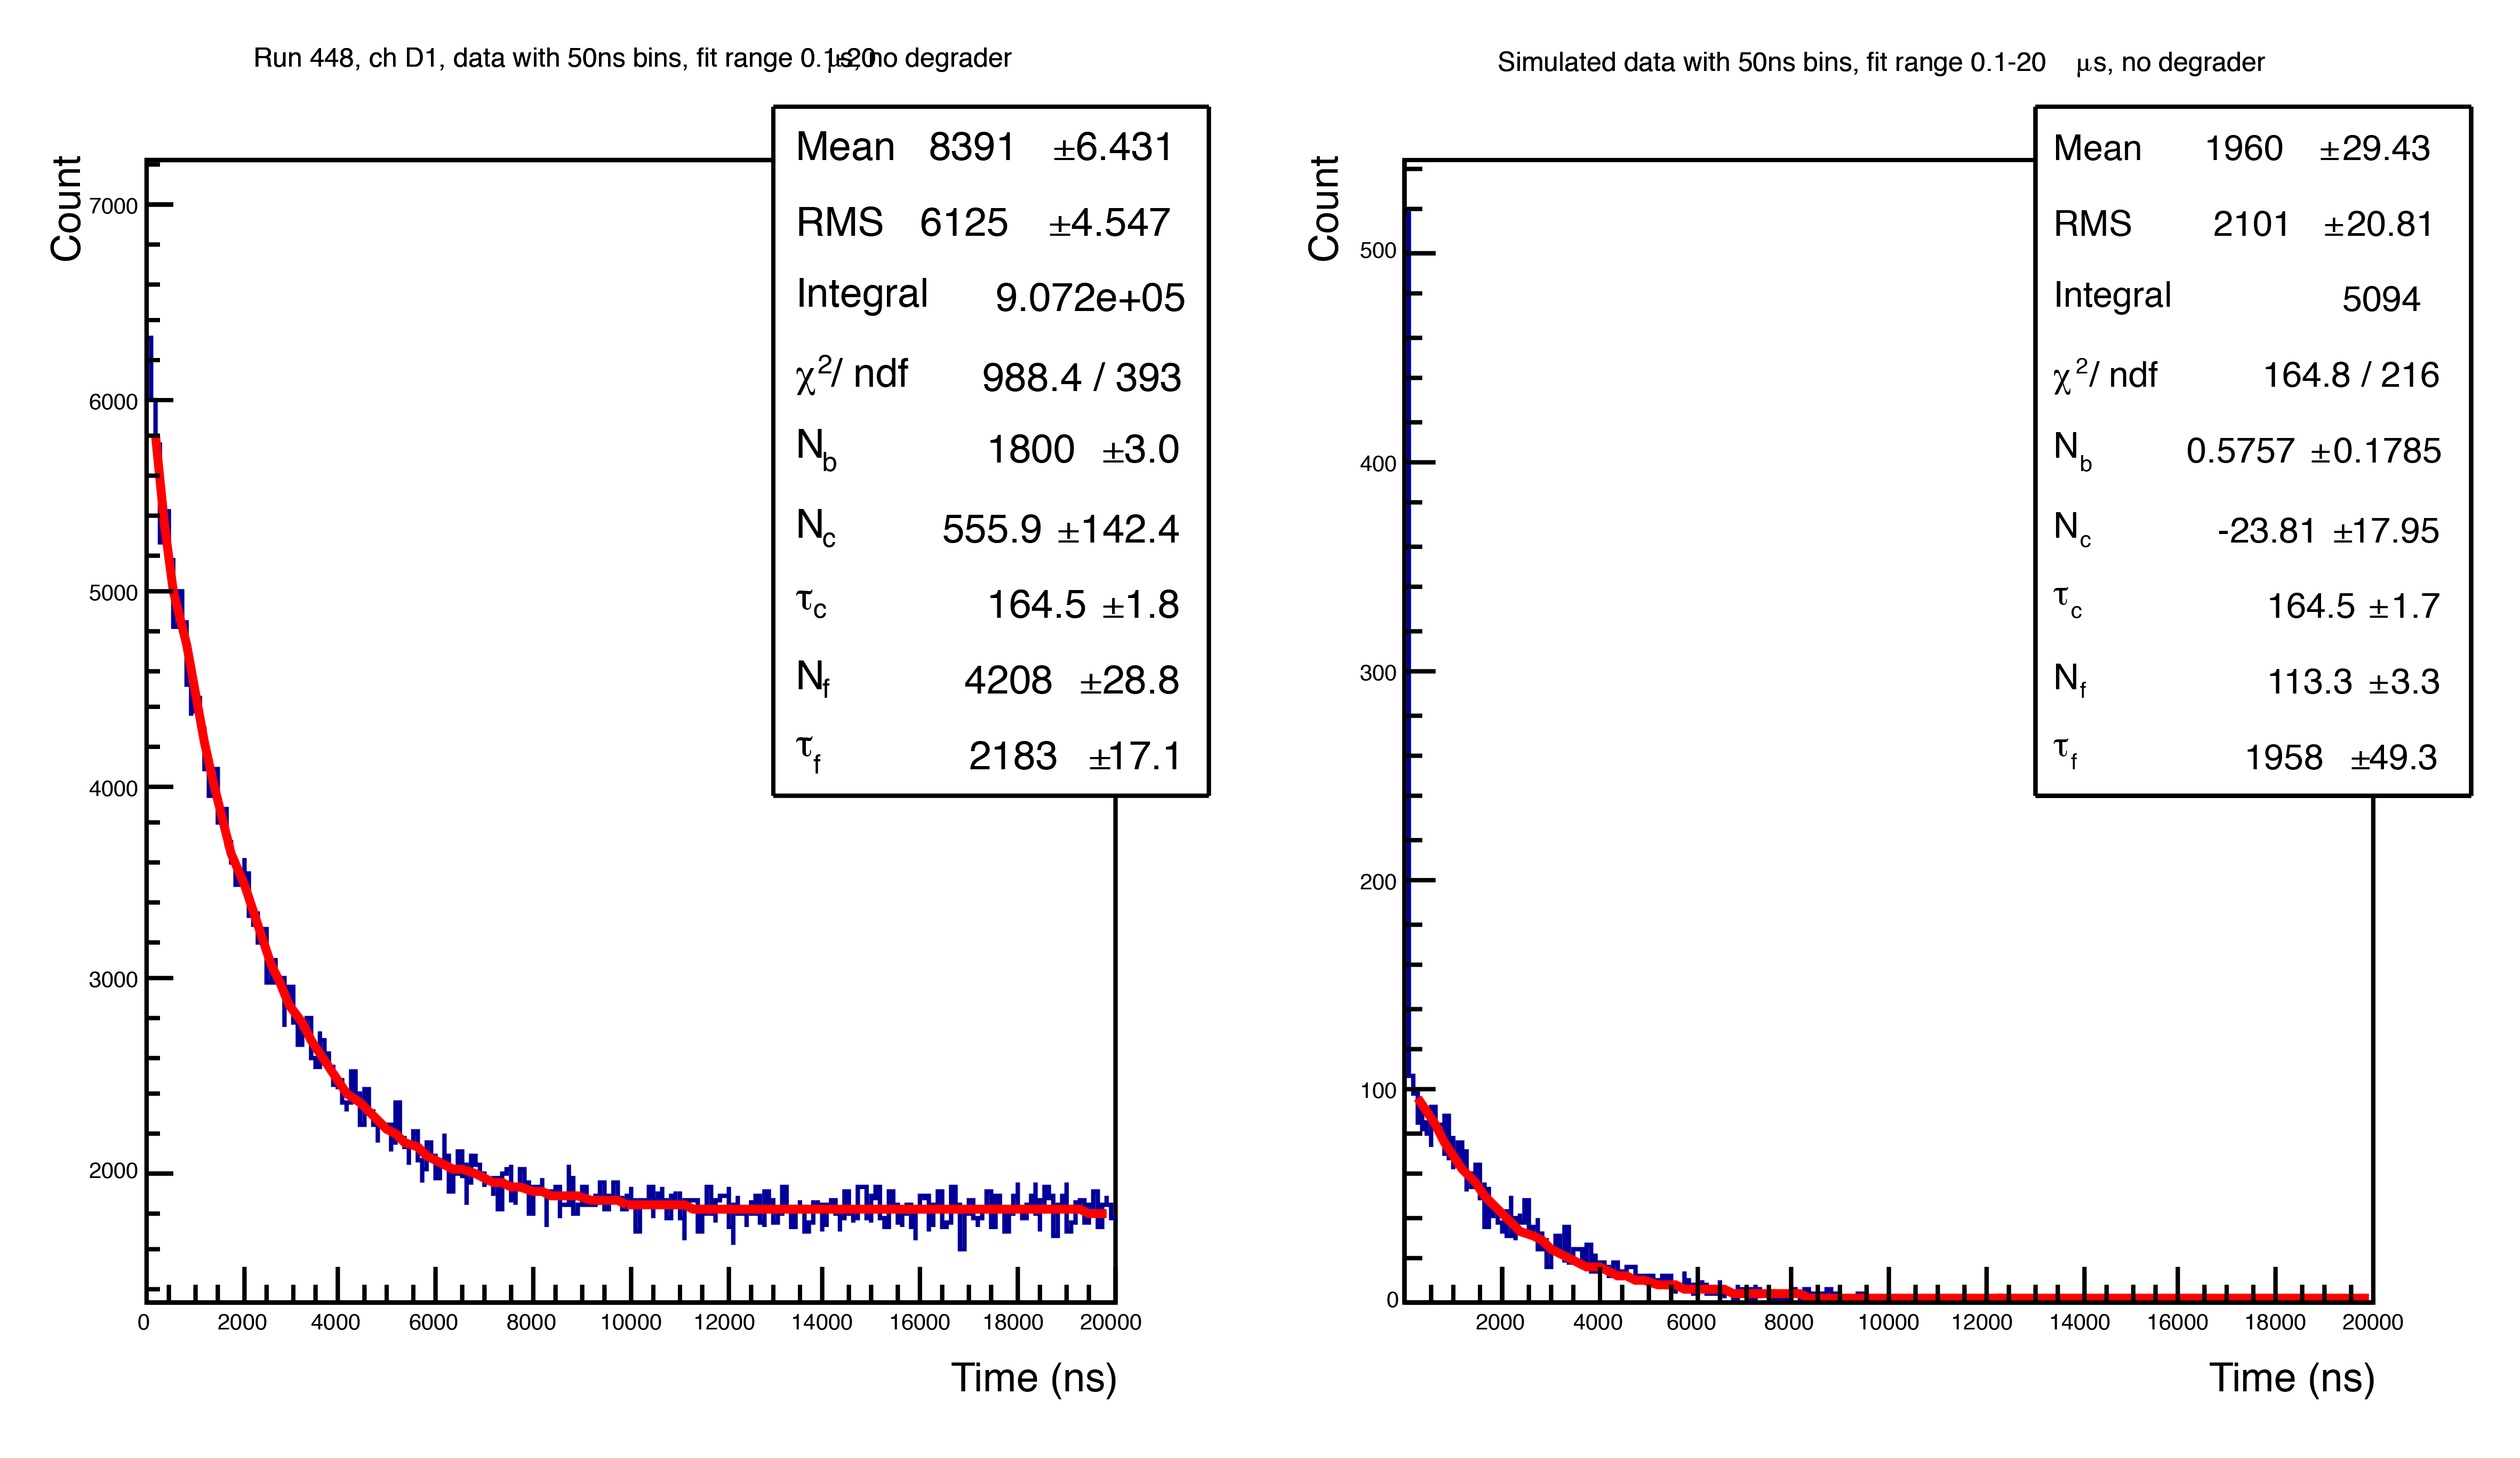
\includegraphics[width=\textwidth]{images/example_fits_data_and_sim.png}
%     \caption{Example of typical histograms for both simulation and data. Each has been fitted with equation~\ref{equ:fit} using initial fit settings matching those in table~\ref{tab:typical_fit_values}. The run used was 448, channel D1, i.e. no degrader, and simulation was for air only.}
%     \label{fig:example_fits_data_and_sim}
% \end{figure}
% 
% \begin{figure}[htbp]
%     \centering
%         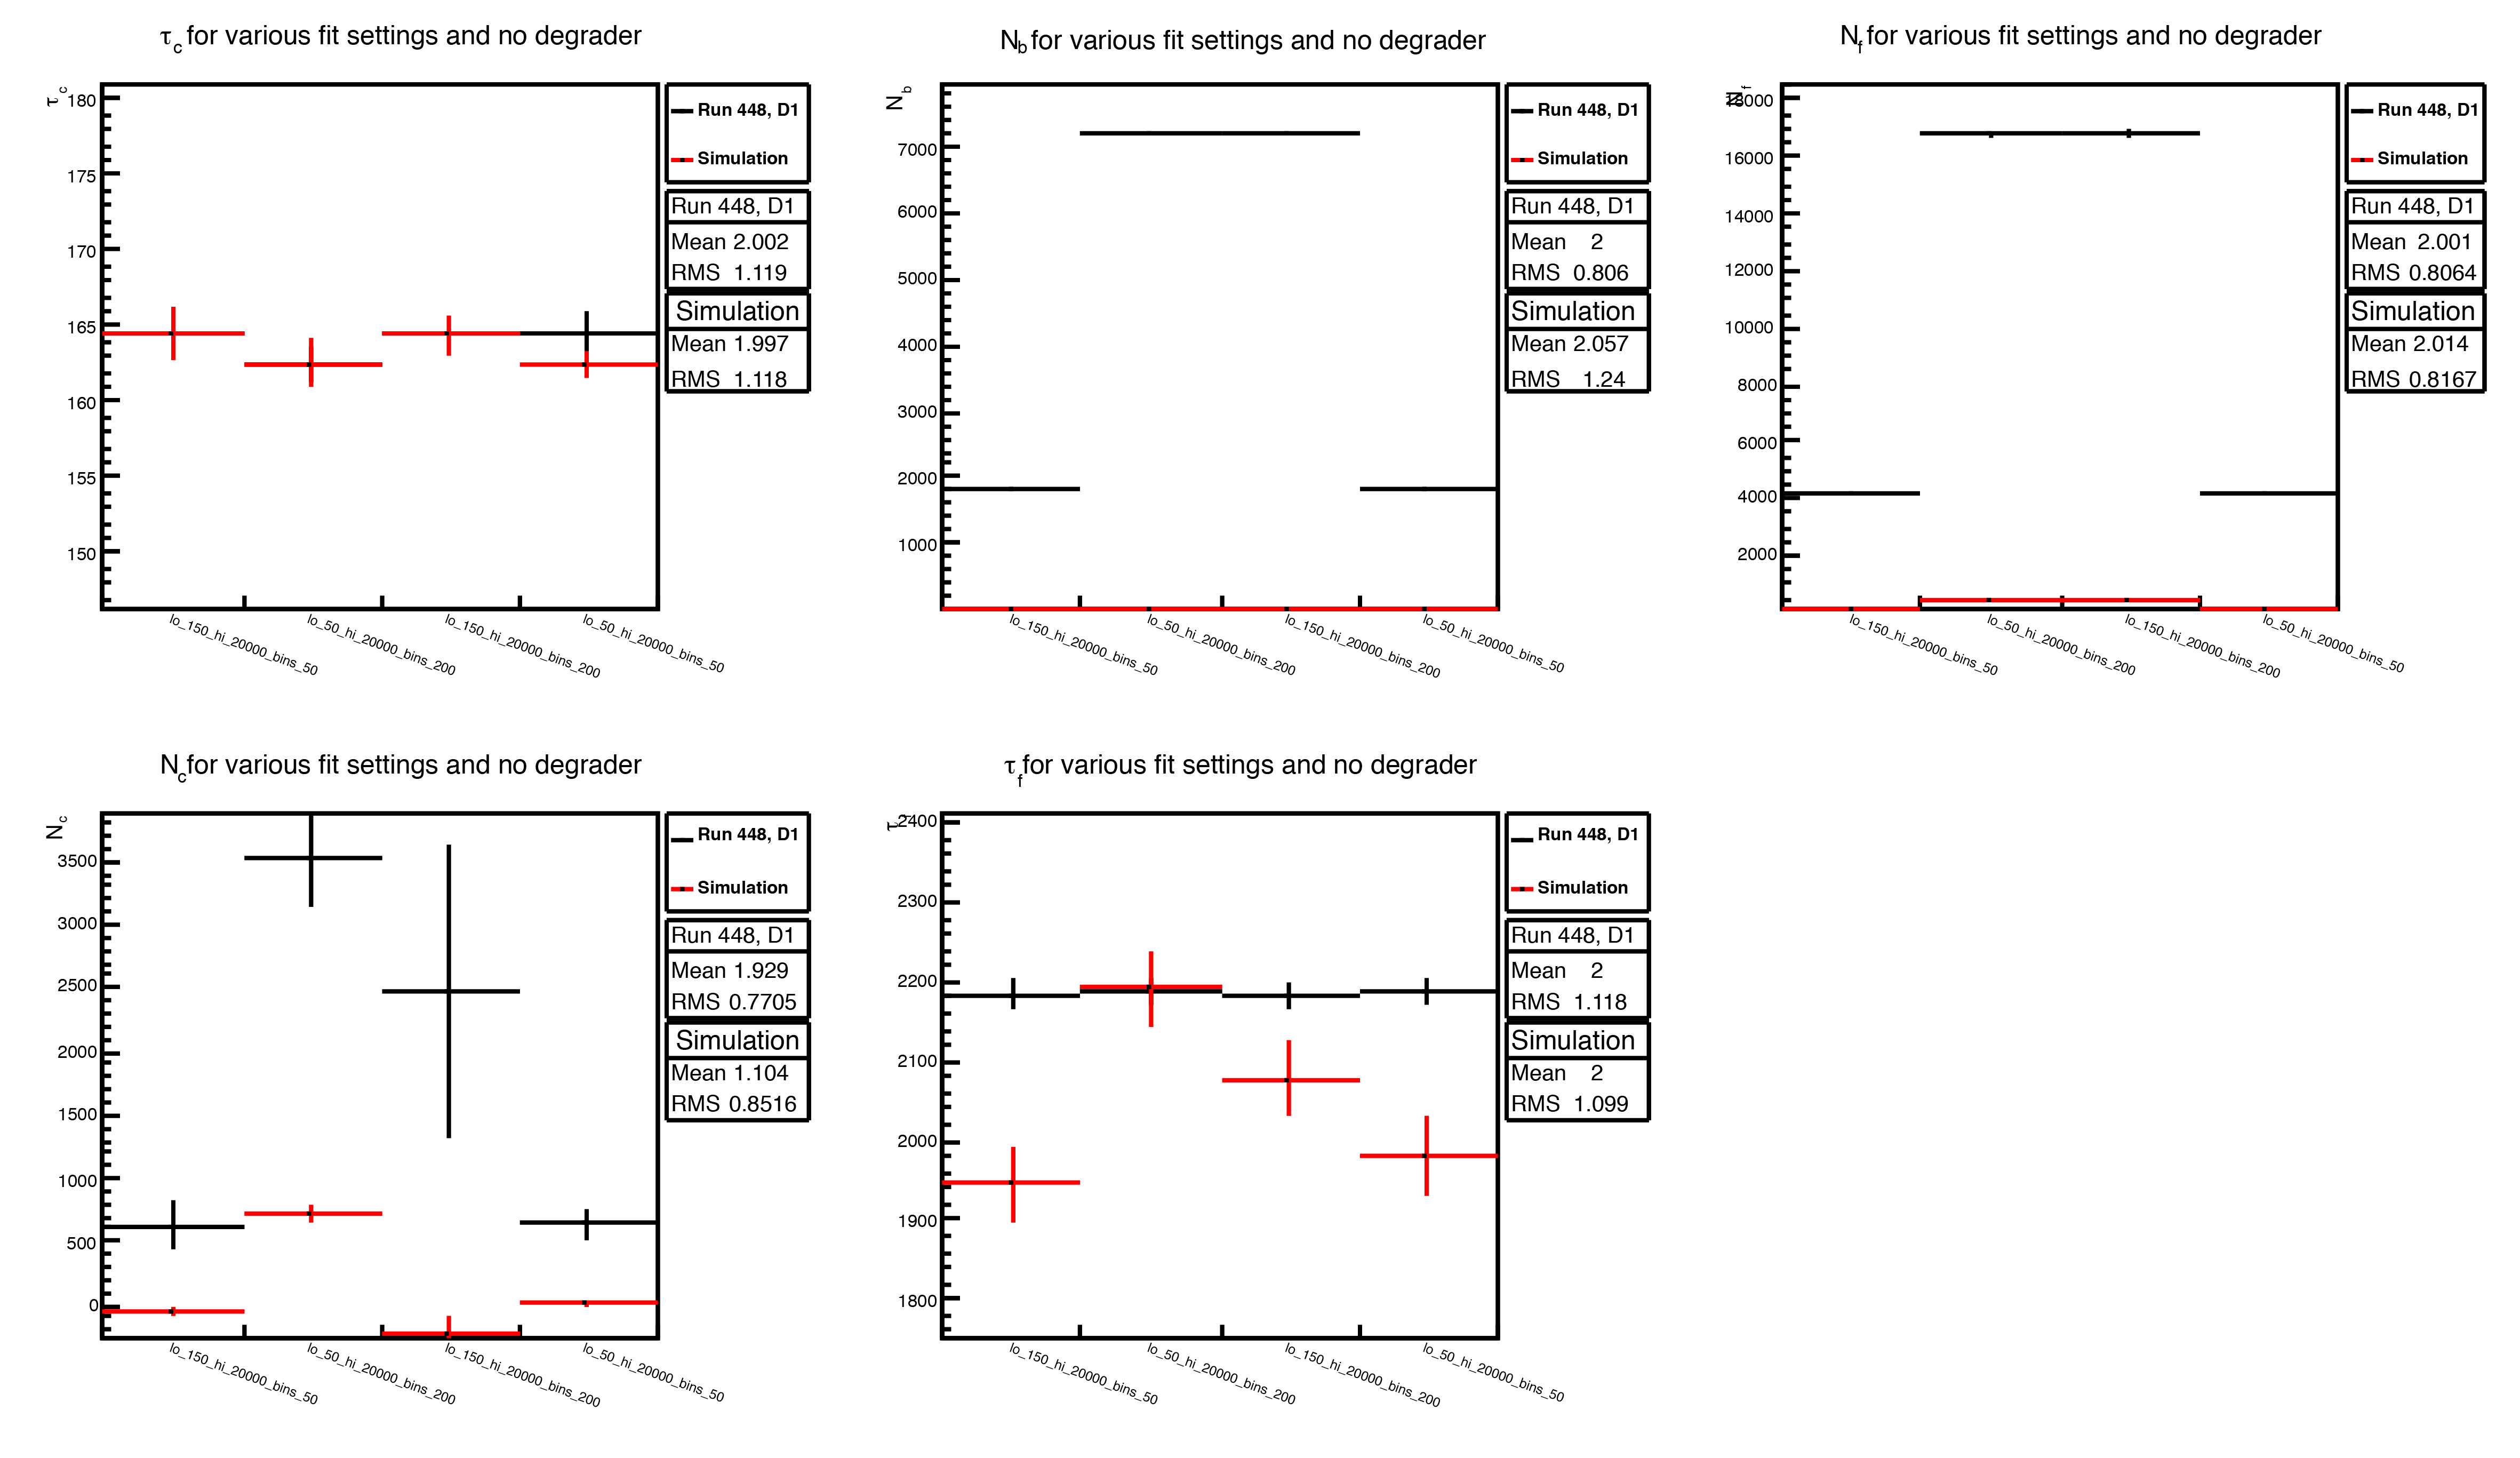
\includegraphics[width=\textwidth]{images/sim_vs_data_parameter_WRT_settings.png}
%     \caption{Demonstration of the variance of fitted parameters with respect to the initial fit settings. The x axis labels list the settings used for that bin e.g. `lo\_100\_hi\_20000\_bins\_50' corresponds to a lower bound of 100~ns, an upper bound of 2\mus{} and a bin width of 50~ns. Bare in mind that the $N$ values have not had any compensation for acceptance etc. applied so difference between simulation and data is expected.}
%     \label{fig:image_sim_vs_data_parameter_WRT_settings}
% \end{figure}
% 
% The largest changes to the fit are due to the fit settings figure~\ref{fig:example_fits_data_and_sim} shows examples of simulated and real data with their respective fits . These determine the range that is fitted and the smoothness of the data that the fit is attempted on. The lower bound of the range probably has the largest affect on the fit. It is obvious that a large enough lower bound will utterly remove the region in which the copper component is dominant (i.e.\ $\lesssim$ 200~ns), to avoid this the minimum value of 50~ns is usually chosen which corresponds to the maximum anti-coincidence period of the trigger. The upper bound has very little affect for any reasonable value ($>$15\mus) as that portion of the histograms is usually flat. The bin width has an important part to play as it the prime method of smoothing data. 
% 
% \begin{figure}[htbp]
%     \centering
%         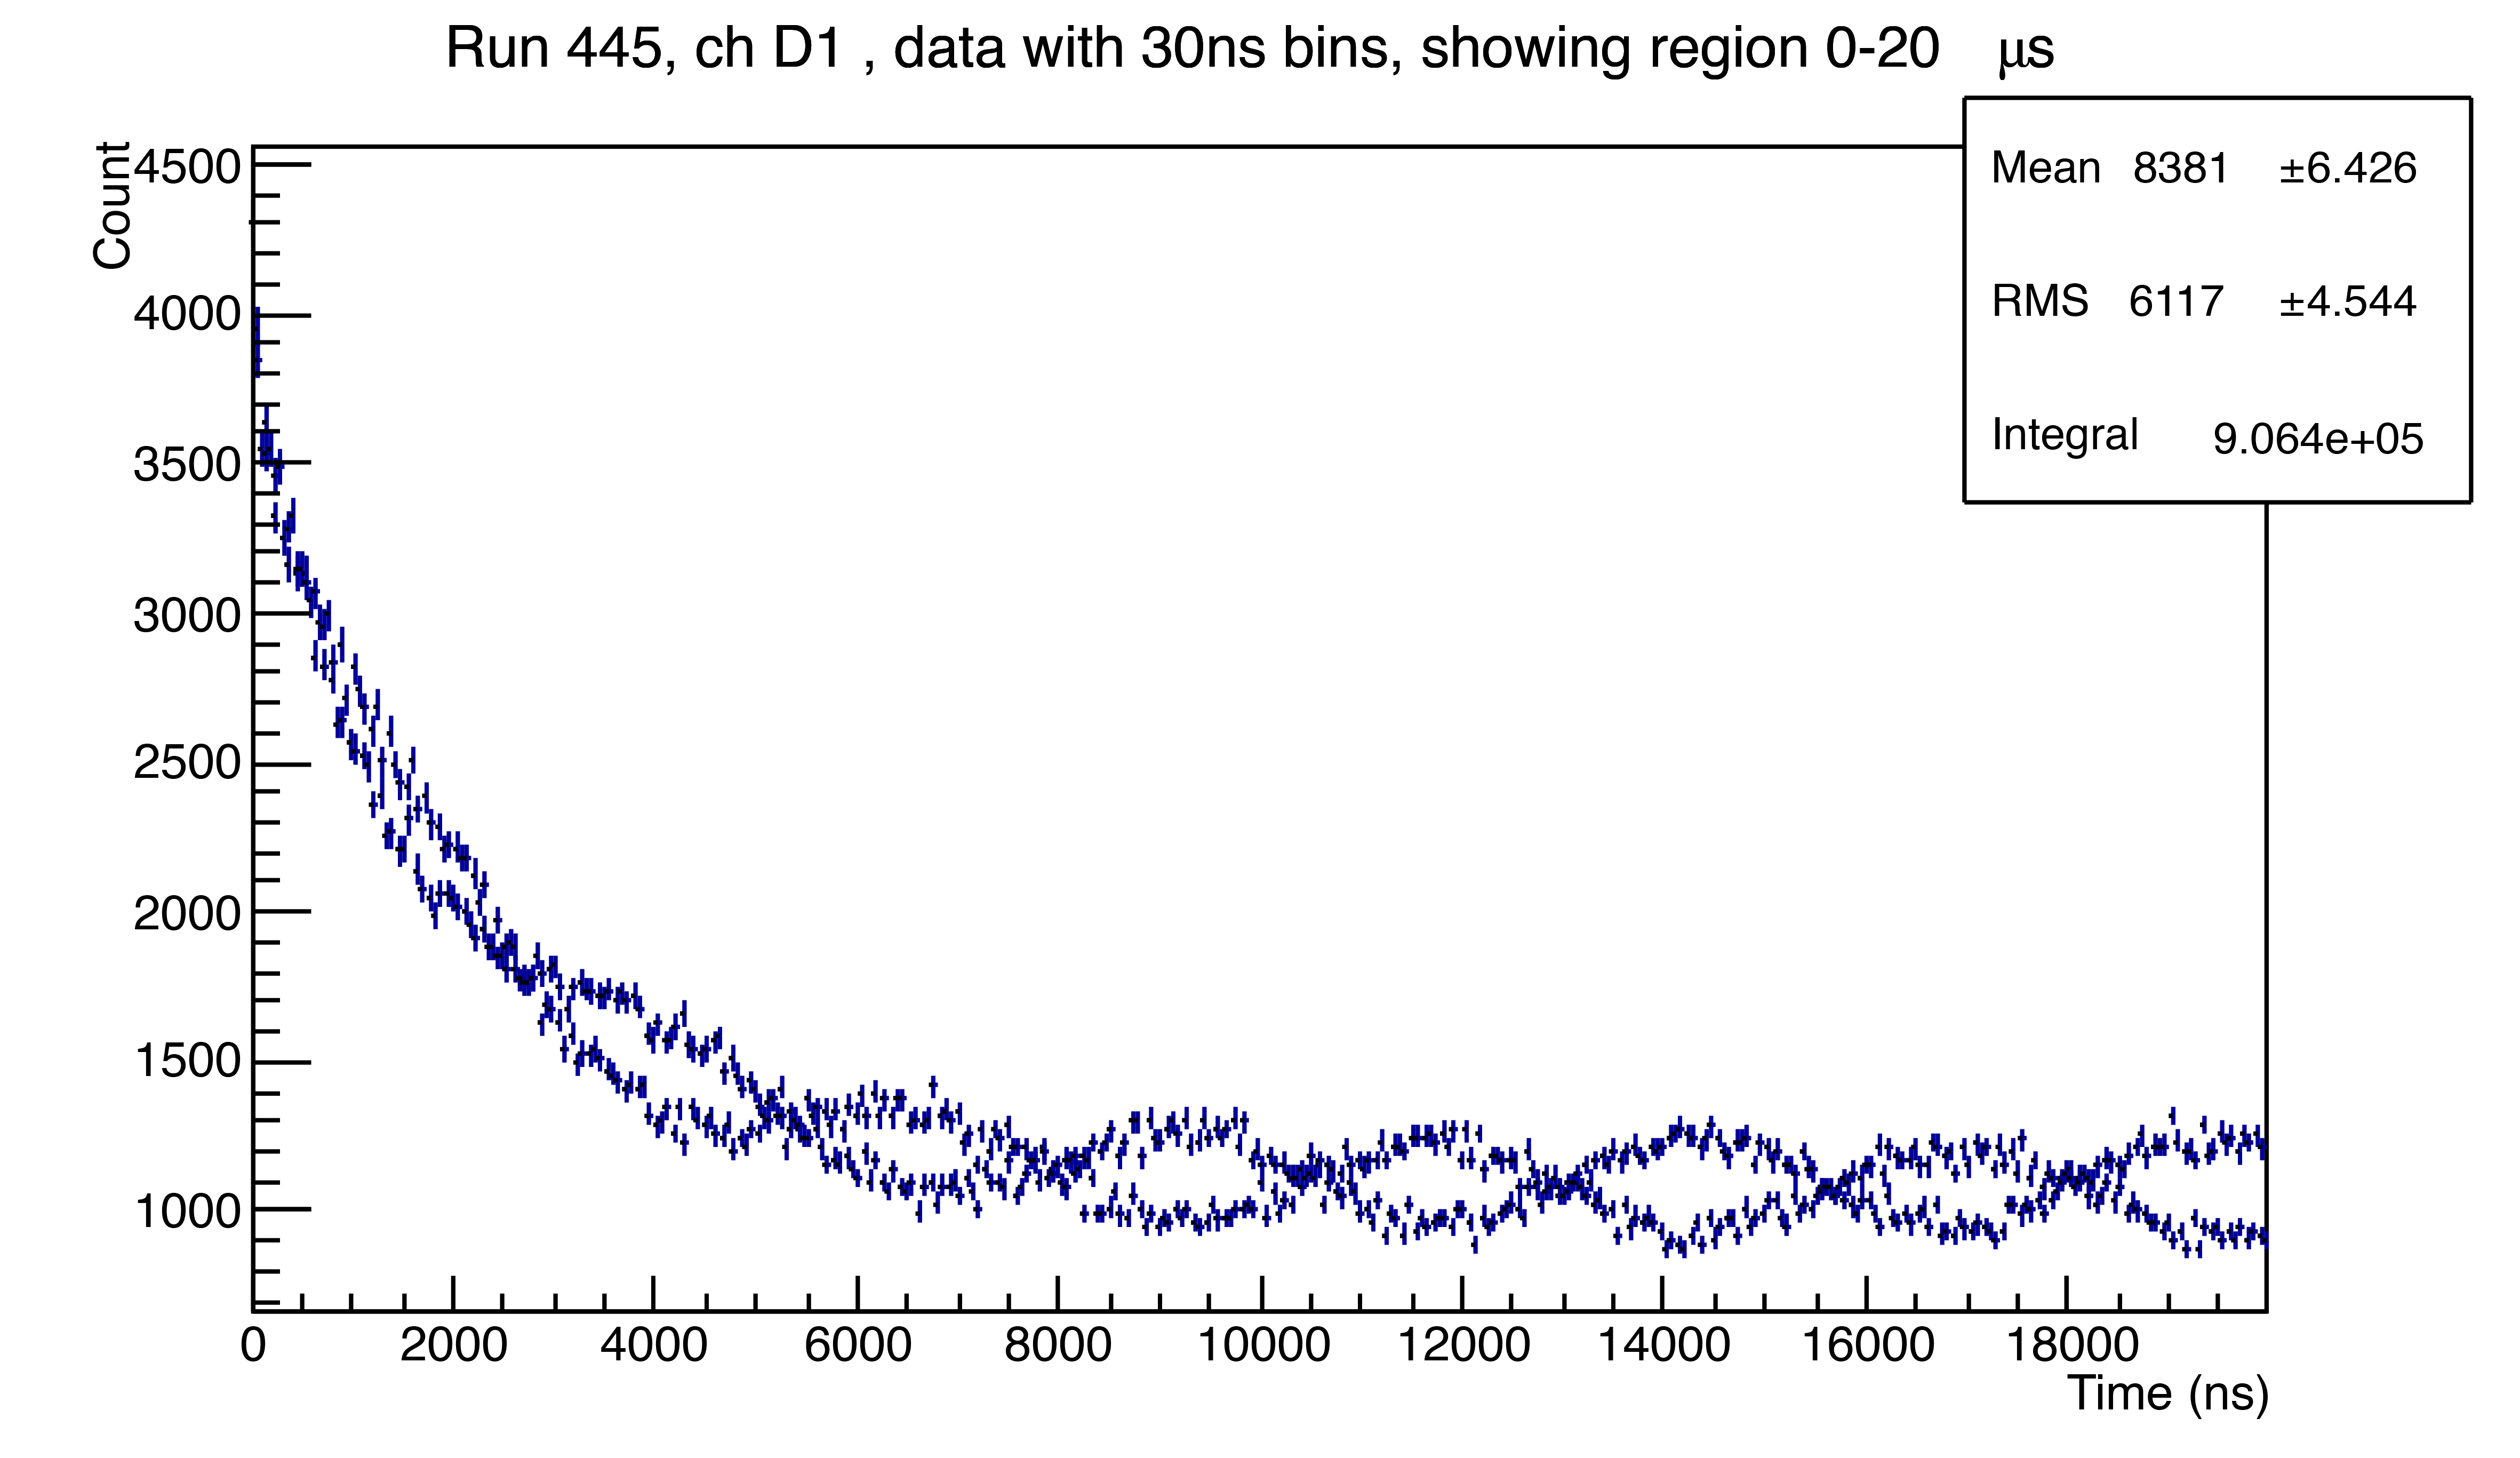
\includegraphics[width=\textwidth]{images/example_noise.png}
%     \caption{Example of the noise seen in the data. Both the high ($\sim$16~MHz) and low ($\sim$45~kHz) frequency components are clearly visible. An enlarged view of the tail of this distribution is given in figure~\ref{fig:example_noise_zoom}}
%     \label{fig:example_noise}
% \end{figure}
% %
% \begin{figure}[htbp]
%     \centering
%         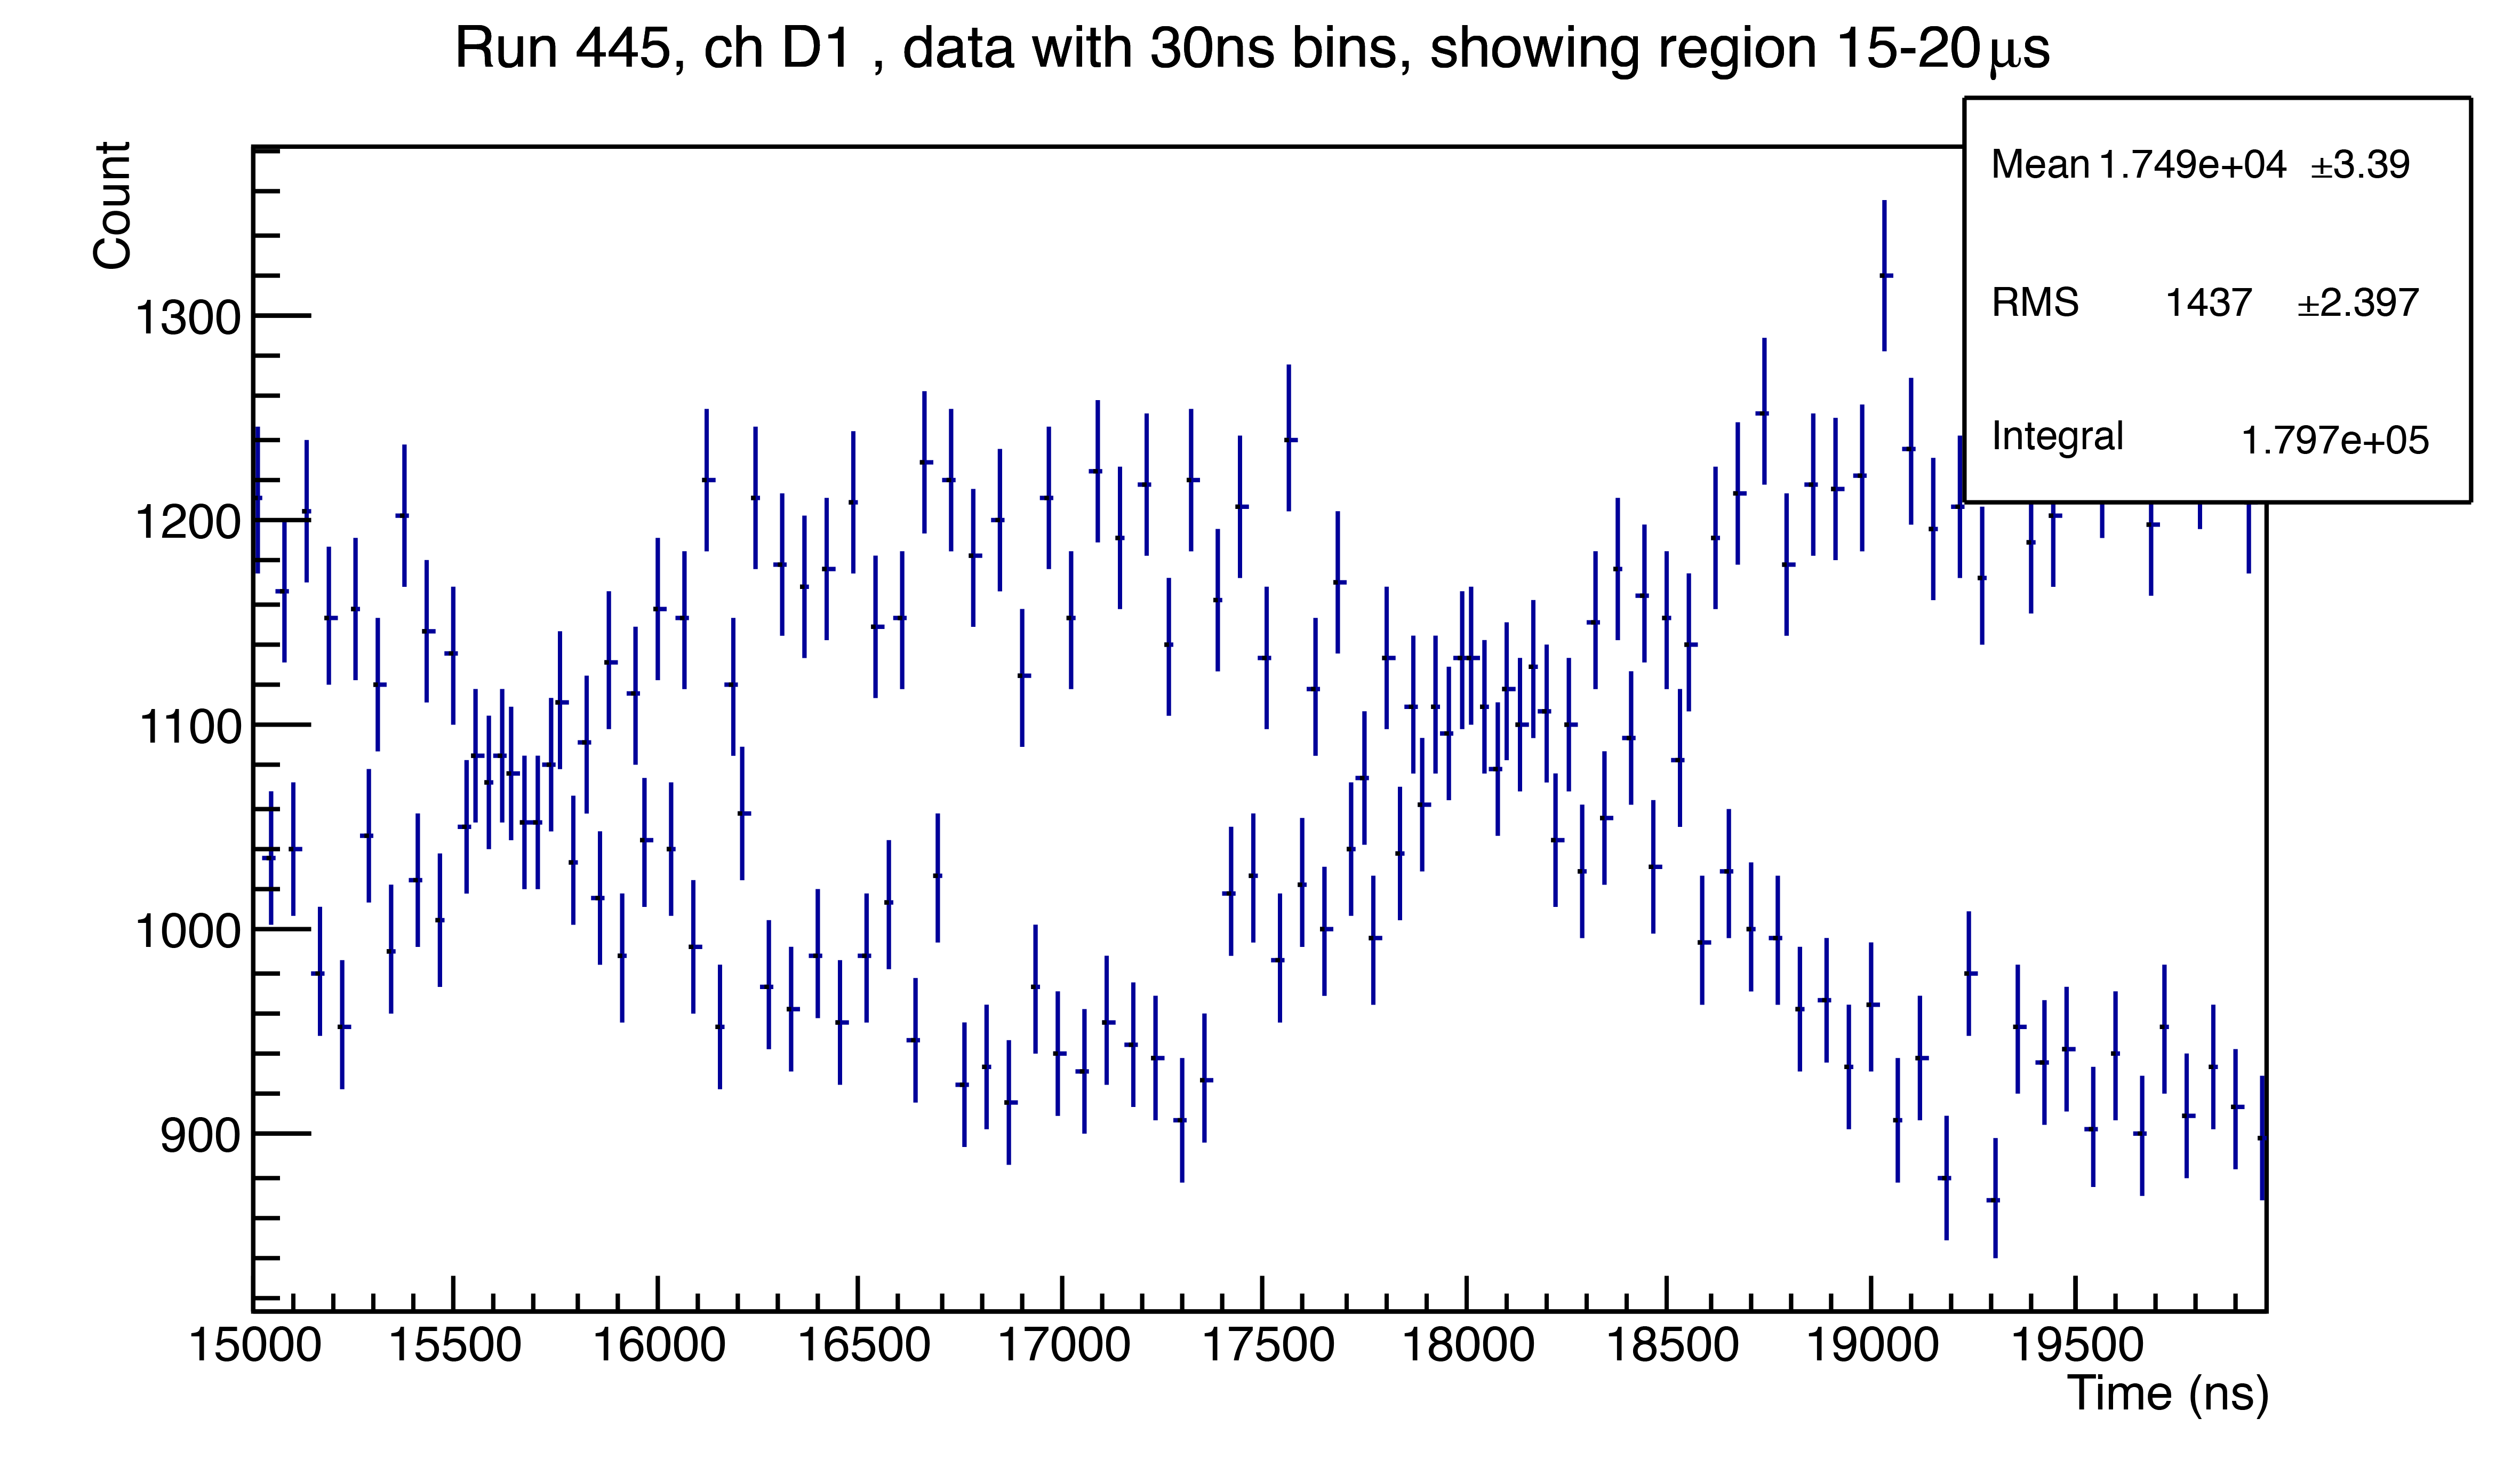
\includegraphics[width=\textwidth]{images/example_noise_zoom.png}
%     \caption{Enlarged view showing the high frequency component of the noise more clearly.}
%     \label{fig:example_noise_zoom}
% \end{figure}
% 
% Smoothing the data appears to be very important judging by the noise seen in figure~\ref{fig:example_noise}. As can be seen there appears to be a high frequency component with a period $\sim$60~ns (frequency $\sim$16~MHz) imposed upon a much slower carrier period $\sim$2.2\mus{} (frequency $\sim$45~kHz). Using a suitable bin width (e.g. 100~ns) the high frequency component can be removed and the overall affect of the noise greatly reduced (see figure~\ref{fig:example_smoothing}).
% 
% \begin{figure}[htbp]
%     \centering
%         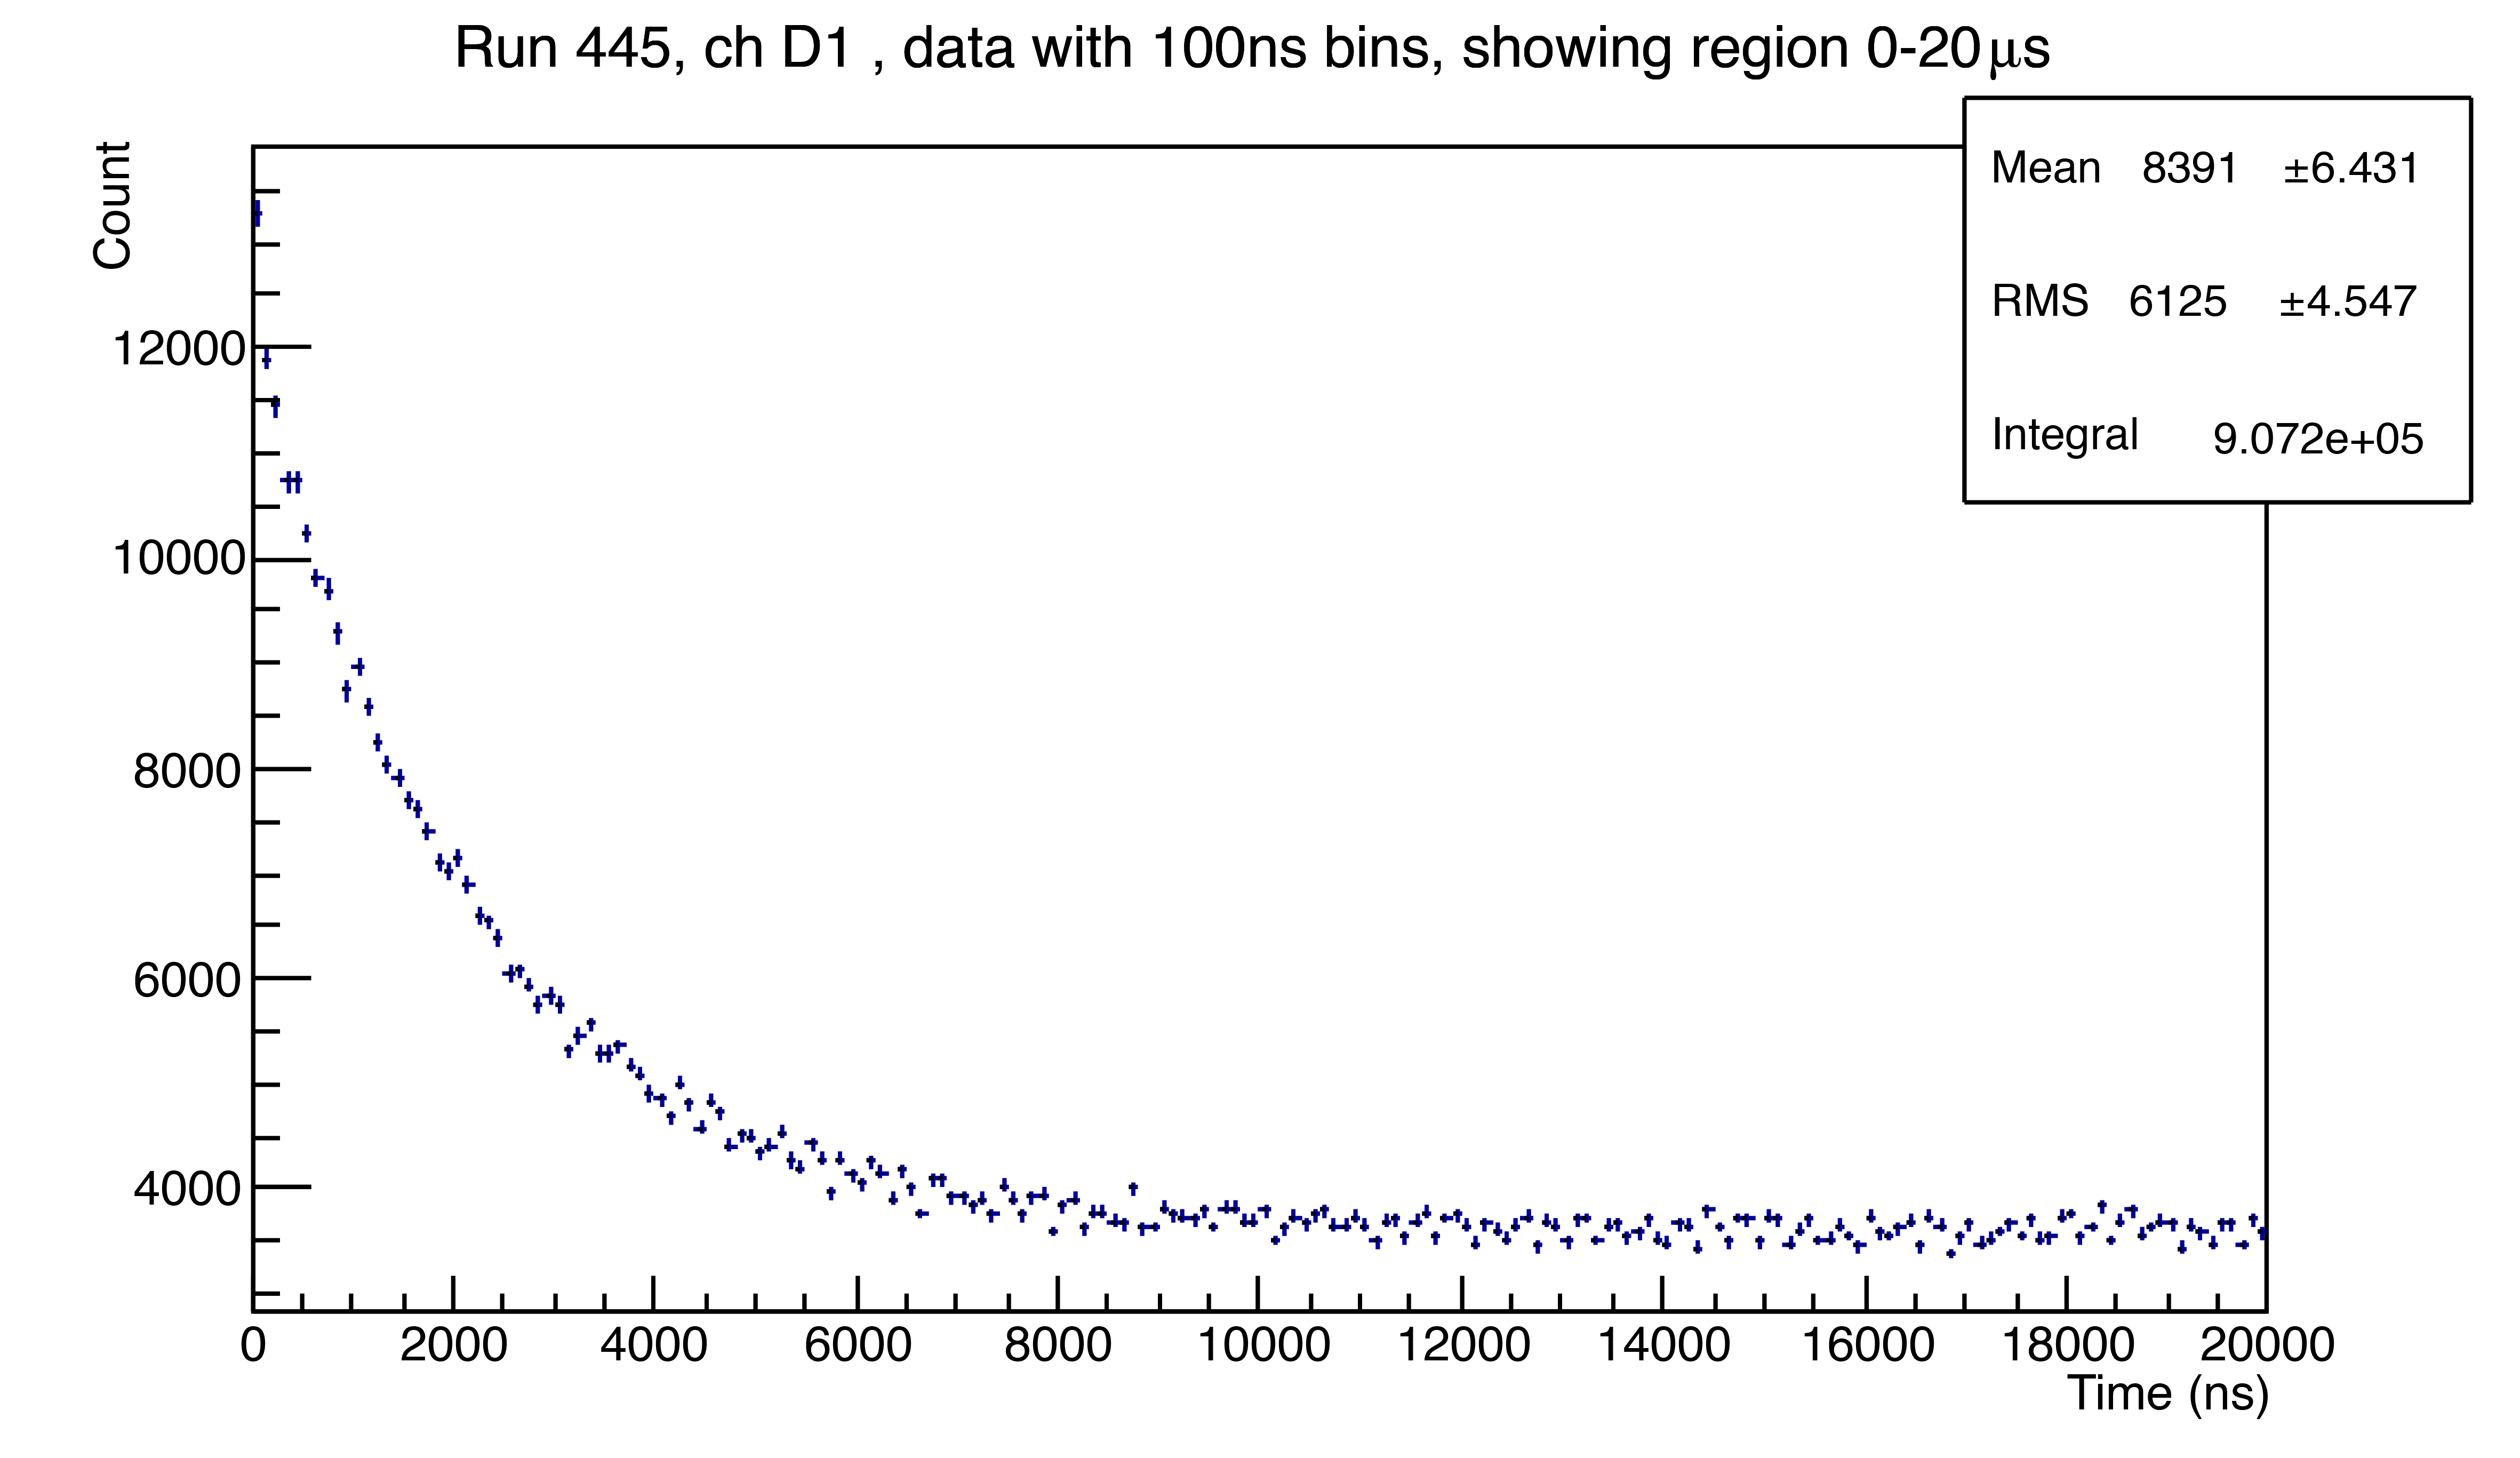
\includegraphics[width=\textwidth]{images/example_smoothing.png}
%     \caption{Example of the data once suitably large bins (in this case 100~ns) have been applied in order to remove high frequency noise cf.\ figure~\ref{fig:example_noise}.}
%     \label{fig:example_smoothing}
% \end{figure}
% 
% The initial fit parameters were set by `eyeball' to approximations of their expected value, if this were not done ROOT would set all values to 0. A reasonably large range of values was chosen to avoid degeneracies (this is especially important to make sure that each fit corresponds to its label). $\tau_{c}$ is generally fixed to a range of $\pm$1~ns about its canonical value of 163.5~\cite{PhysRevC.35.2212} as this is a known value reasonably different compared to the other muonic lifetimes\footnote{The lifetimes for the other major materials in the detector are: Hydrogen 2194.903$\pm$0.066, Carbon 2026.3$\pm$1.5~ns, Nitrogen 1906.8$\pm$3.0~ns, Oxygen 1795.4$\pm$2~ns~\cite{PhysRevC.35.2212}. Where the scintillator is assumed to be mostly carbon and hydrogen and the air mainly nitrogen and oxygen.}. It is worth noting that only the negatively charged muons can form muonic atoms and so the copper component of the fit makes a reasonable approximation to this number whilst the free component will be composed of primarily of positively as well as negatively charged muons.
% 
% Once the histograms were fitted the fit parameters were extracted and used to create sub-functions corresponding to the individual components. Using ROOT's `Integral' and `IntegralError' functions the number of decays for each channel corresponding to each component could then be calculated. Equally summing over all the channels in a run the total number of muons for that run could be calculated.
% % subsection the_implementation (end)
% % section fitting_and_integration (end)
% %%%%%%%%%%%%%%%%%%%%%%%%%%%%%%%%%%%%%%%%%%%%%%%%%%%%%%%%%%%%%%%%%%%%%%%%%%%%%%
% \section{Muon Yield} % (fold)
% \label{sec:muon_yield}
% Once the number of muons for each run is known the muon yield is ultimately a matter of scaling. The formula used is:
% \begin{align}
%     Y = \frac{N_{mu}}{\epsilon \times A \times D \times t_{r} \times I}
% \end{align}
% Where $Y$ is the yield, $N_{mu}$ the number of muons for that run, $\epsilon$ is the detector efficiency, $A$ the acceptance for that degrader thickness, $D$ is the dead-time, $t_{r}$ is the run time in seconds and $I$ is the proton current. The detector efficiency was not measured for this experiment but based on previous experiments (e.g. detector efficiency for MuSIC~3) is set to 50\% and incorporated into both calculations for simulated and real data. 
% % chapter muon_momentum_spectrum (end)
% %%%%%%%%%%%%%%%%%%%%%%%%%%%%%%%%%%%%%%%%%%%%%%%%%%%
% % part characterising_the_beam (end)
% %%%%%%%%%%%%%%%%%%%%%%%%%%%%%%%%%%%%%%%%%%%%%%%%%%%
%  
    \part{Clock and Control interface for the Large Pixel Detector} % (fold)
\label{prt:lpd_ccc_interface}

\section{Conventions} % (fold)
\label{sec:conventions}
Throughout this document there are several typographical conventions that are observed (see table~\ref{tab:typography}).
% CAPS           = states          e.g. IDLE, 
% bold(CAPS)     = generic         e.g. BUNCH_LENGTH 
% textttt{CAPS}  = commands        e.g. SET_TRIGGER_FLAG
% textttt{lower} = ports/signals   e.g. start_i
% 
% 
% veto from ccc->veto to asic 7 clk
% start from ccc->start to asic 6 clk
% above due to requirements to sync to 4.5 MHz
\begin{table}[htbp]
  \begin{center}
  \begin{tabular}{c|c}
    Type or prefix                  & Meaning                             \\
    \hline                                                   
    \texttt{lower mono-spaced font} & Port or signal names.               \\
    lower normal font               & Port or signal names (tables only). \\
    CAPS                            & Names of generics.                  \\
    \textbf{BOLD CAPS}              & Named states of a state-machine.    \\
    \texttt{MONO-SPACED CAPS}       & Command words.                      \\
    CAPS                            & Command words (tables only).        \\
    0xYYYY                          & Hexadecimal number (YYYY in base 16)\\
    0bYYYY                          & Binary number (YYYY in base 2)      \\
  \end{tabular}
  \end{center}
  \caption{Description of typographic conventions.}
  \label{tab:typography}
\end{table}
% section conventions (end)
%%%%%%%%%%%%%%%%%%%%%%%%%%%%%%%%%%%%%%%%%%%%%%%%%%%
\chapter{Introduction} % (fold)
\label{cha:lpd_ccc_introduction}
\section{The European X-ray Free-Electron Laser: an overview} % (fold)
\label{sec:xfel_an_overview}
This is a discussion of the work carried out designing the firmware for the Clock and Control Card (CCC) interface of the Large-Pixel Detector (LPD) for use at the European X-ray Free-Electron Laser (EuXFEL). There will be a brief discussion of EuXFEL, its aims, the detectors and control systems then a more in-depth look at the design, implementation and testing of the interface.

EuXFEL is a 3.4~km Free-Electron Laser (FEL) being constructed below Hamburg, Germany. The project is scheduled to begin operation in 2016 with commissioning beginning in 2015. EuXFEL is built upon expertise and concepts prototyped at the Free-electron Laser in Hamburg (FLASH) which is operated by DESY although EuXFEL will be operated as an independent research facility. The aim of EuXFEL is produce a coherent X-ray beam with peak brilliance of 10\(^{33}\)~photons/s/mm\(^2\)/mrad\(^2\)/0.1\%BW; a pulse duration of \( \sim \)100~fs and a wavelength down to \( \sim \)0.1~nm.


\subsection{Synchrotrons and FELs} % (fold)
\label{sub:synchrotrons_and_fels}
X-rays are produced from electrons via synchrotron radiation in which the electron is accelerated through a magnetic field causing it to curve and lose energy, this energy is lost as photons which are X-rays. Synchrotron sources use Linear Accelerators (Linacs) to accelerate electrons before injecting them into a storage ring where they are passed through bending magnets to produce X-rays. The original synchrotron sources used the natural curvature of their storage ring to produce X-rays more modern designs use special sets of magnets (called `undulators') that very rapidly change the electron's course to produce X-rays, by changing the configuration the undulators the X-ray properties can also be adjusted. 

The use of undulators is key to producing a FEL, rather than at a synchrotron where they are used just to produce X-rays at a FEL, by adjusting the undulators' properties, the electrons can be forced to interact with the X-rays they emit, through this interaction a single bunch can be forced into many smaller bunches as the slower electrons absorb the X-rays of the faster electrons through a process called `micro-bunching'. Ultimately through micro-bunching the electrons in the beam end up in phase with one-another and rather than LASEing start to self-amplify, stimulated-emission (SASE)\footnote{Technically `FEL' is a misnomer, it should be FES.} this produces a similar effect to a laser in that the resultant light is coherent and with the added bonus of forming very short pulses.
% subsection synchrotrons_and_fels (end)
%%%%%%%%%%%%%%%%%%%%%%%%%%%%%%%%%%%%%%%%%%%%%%%%%%%
\subsection{X-ray production at EuXFEL} % (fold)
\label{sub:x_ray_production_at_euxfel}
At EuXFEL electrons are accelerated to 17.5~GeV using a superconducting linac and the X-rays are produced in one of three SASE undulators which can be combined with conventional undulators to produce photon energies from 25~keV to 0.26~keV which correspond to wavelengths of between 0.05~nm and 4.7~nm the proposed layout can be seen in figure~\ref{fig:XFEL_layout}. EuXFEL is predicted to be able to supply 27,000 pulses of X-ray light (`bunches') per second, with each pulse having a duration of \( \sim \)100~fs. The bunches are split over 10 `trains' per second, each containing up to 2,700 bunches each and lasting \( 600~\mu\)s. The predicted cumulation of all this is a peak brilliance of 10\(^{33}\)~photons/s/mm\(^2\)/mrad\(^2\)/0.1\%BW, for the comparison the energy and peak brilliance of several existing sources (FEL and synchrotron) is given in figure~\ref{fig:xfel-brightness}, as can be seen FELs (FLASH, LCLS) have a much higher peak brilliance although, generally, with a reduced range in energy.
\begin{figure}[htbp]
  \centering
    \includegraphics[width=.9\textwidth]{images/Other/XFEL_layout.png}
    % \includegraphics[width=.9\textwidth]{4_appendix_XFEL/images/Other/XFEL_layout.png}
  \caption{Schematic of the beam-lines for EuXFEL, black denotes electrons whilst red corresponds to X-rays.}
  \label{fig:XFEL_layout}
\end{figure}

\begin{figure}[htbp]
  \centering
    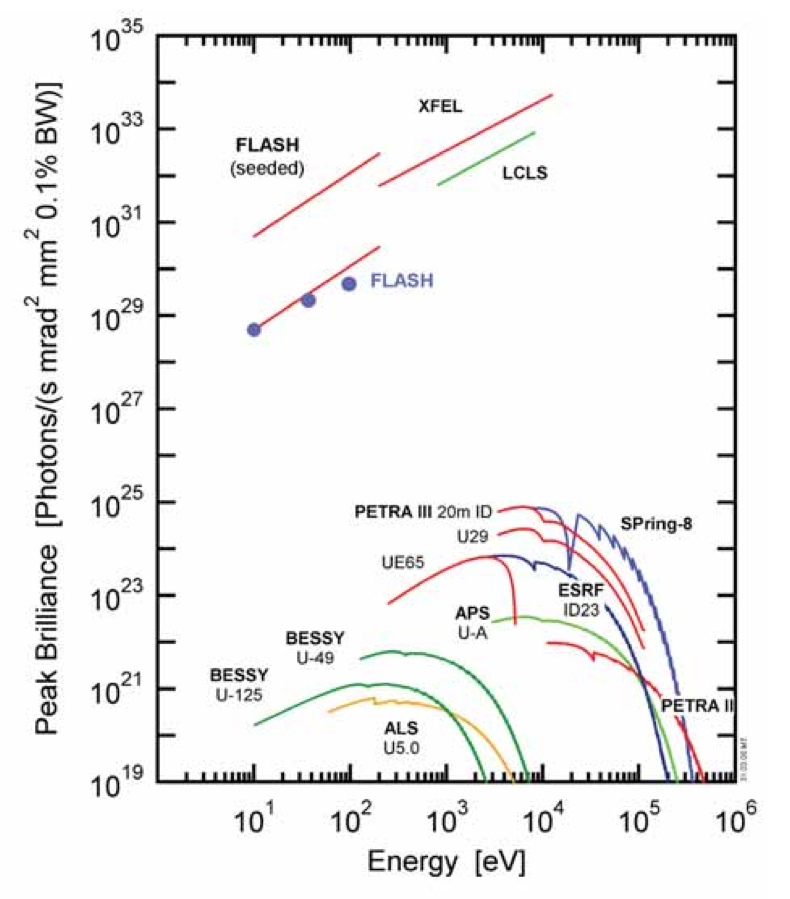
\includegraphics[width=.9\textwidth]{images/Other/XFEL-comparitive_energy-brightness.png}
  \caption{Plot of peak X-ray brilliance against energy for a range of current sources as well as the predicted values for EuXFEL (here labelled `XFEL'). The blue dots show measured peak brilliance for several energies at the existing FLASH facility, `FLASH (seeded)' is a proposed extension using a micro-bunch `seeded' electron beam.}
  \label{fig:xfel-brightness}
\end{figure}

% subsection x_ray_production_at_euxfel (end)
%%%%%%%%%%%%%%%%%%%%%%%%%%%%%%%%%%%%%%%%%%%%%%%%%%%
\subsection{Scientific Motivation} % (fold)
\label{sub:scientific_motivation}
There are two primary problems with more traditional synchrotrons: incoherent light and pulse length. As the light is produced in a long bunch of electrons it has no over-all phase this means that only samples that are crystalline (or can be crystallised, i.e.\ grown into a repeating pattern) can be imaged. Many structures form only poor crystals or can't form them at all. The X-ray pulse length that synchrotrons produce, whilst under normal operating conditions, are generally of order 10--100~ps~\cite{xfel_detector_requirements} obviously this places a lower limit on the speed of things that you can `film', again limiting the range of experiments that can be carried out. FELs solve both of these problems by producing coherent light that can have a very short pulse length, additionally because of the SASE process the peak brilliance of a FEL is vastly increased (see figure~\ref{fig:xfel-brightness}).

The primary aim of EuXFEL is to study conditions previously unseen in a laboratory setting. This aim is achieved through three core properties of EuXFEL: `coherence, ultra-high brilliance and time structure'~\cite{xfel_tdr} the combination of these gives access to three broad areas of study: the tiny, the fast and the extreme. Because of the limitations of incoherent light, pulse length and brilliance none of these regimes are easily studied at synchrotrons.

The imaging of the tiny relies on the wavelength of the light used being comparable to the scale of the structure to be imaged. At EuXFEL as well as having X-ray wavelengths sufficient to image molecules, due to the coherent nature of the light non-repeating structures can also be imaged unlike at traditional synchrotrons. Whilst the brilliance of the beam will destroy most samples very quickly tests at FLASH show that enough time remains to produce a detailed image of the sample, even if it has not been crystallised. This means that larger structures can be imaged at an atomic scale (e.g.\ entire viruses) or structures that won't crystallise or only form very small, low quality crystals (e.g.\ protein membranes).

EuXFEL's time-structure, provides the potential of the second regime, speed. As each individual flash lasts less than \( \sim \)100~fs and each train comprising of 2,700 flashes it's possible to `film' processes as they occur. This will make it possible for researchers to understand what happens during a phase transition or when a material reverses its magnetisation by watching it happen in high detail and without suffering the motion-blur of slower systems.

The final regime, the extreme, is driven by EuXFEL's brilliance. Able to recreate intense temperatures and pressures EuXFEL can ue this to create environments not normally seen on Earth. For example: the propagation of shockwaves through a plasma or to image the stresses on a component under extreme magnetic fields.
% subsection scientific_motivation (end)
% section xfel_an_overview (end)
%%%%%%%%%%%%%%%%%%%%%%%%%%%%%%%%%%%%%%%%%%%%%%%  
\section{Detectors at EuXFEL} % (fold)
\label{sub:detectors_at_euxfel}
In order to achieve EuXFEL's scientific program a broad range of detectors are required. For almost all planned experiments there is a need to image the beam's interaction with the target, the standard solution to this is a 2D pixel detector. This type of detector consists of an array of light sensitive pixels that give both position and intensity information about the incident light, with minor reconstruction an image of the target can then be formed. The basic requirements for the 2D pixel detectors at EuXFEL are~\cite{xfel_tdr}:
\begin{description}
    \item[Swiftness] EuXFEL produces 27,000 X-ray pulses per second, the detector needs to be able to record a large number of these.
    \item[Dynamic range] In any one flash the number of photons received by any portion of the detector can vary massively (between 1 and \(10^5\) photons~\cite{lpd_manual}) this information needs to be preserved with a good signal to noise ratio by the detector.
    \item[Radiation resistance] When fully operational EuXFEL is intended to be used nearly continuously, obviously any detector used has to be able to survive the harsh environment at the end of the beam-line.
\end{description}

There are currently three 2D pixel detectors being built for use at XFEL: Adaptive Gain Integrating Pixel Detector (AGIPD)~\cite{agipd_spec}, DEPFET Sensor with Signal Compression (DSSC)~\cite{dssc_spec} and Large Pixel Detector (LPD)~\cite{lpd_spec}. All three satisfy the above requirements through a variety of technologies.

The main differences between the three detectors are in their approach to the dynamic range: LPD and AGIPD both have three separate gain levels giving them the required range, whilst DSSC uses the non-linearity of its DEPFET to achieve a similar outcome. There are a few other significant differences: DSSC has hexagonal pixels (AGIPD and LPD have square); AGIPD uses dynamic switching to select the appropriate gain for each pixel before storing it in a single pipeline and LPD has an entire pipeline for each gain level (this means that when a narrower gain is required it can be set and all three pipelines used for storage). 

\subsection{The Large Pixel Detector (LPD)} % (fold)
\label{sub:the_large_pixel_detector_lpd}
LPD is a 2D, 1~Mega-pixel detector designed and build by a collaboration of the Rutherford Appleton Laboratory and Glasgow University in the UK. The detector is designed to be modular with a full 1~Megapixel being made up of 16 `supermodules', each supermodule contains a single Front End Module (FEM) that controls and reads out the 128 Application Specific Integrated Circuits (ASICs) each of which has 512 individual pixels i.e.\ each supermodule is 65,536 pixels divided between 128 ASICs and 1 FEM. It is the FEM that then communicates with the rest of EuXFEL via the Clock and Control Card (CCC) and the Train Builder (TB).
    
There are two lines specified for controlling the ASIC during operation: the system clock (\texttt{clk}) and the control (\texttt{cmd}). The FEM's CCC-interface is responsible for receiving the generic signals from the CCC and converting them to those expected by the ASIC. There are a large number of commands that the ASIC expects in order to function (a full list is given in appendix~\ref{app:asic_command_words}). These commands fall into a few general groups: starts, (no-)vetoes\footnote{The ASIC actually uses a `trigger' rather than a `veto', but for consistency with the EuXFEL documentation we will use `no-veto' and `veto' to refer to\texttt{TRIGGER\_FLAG\_SET} and \texttt{NOP} respectively}, stops, resets, and testing. In each of these sets of commands there are generally two or tree individual command words that affect a specific component of the ASIC (e.g.\ reset the write pointer, start the trigger pointer). 
    
Each FEM uses a Xilinx~Virtex-5 Field Programmable Gate Array (FPGA) and two Xilinx~Spartan-3's for control and fan-out, the Virtex-5 has two softcore PowerPC440 processors that manage the resources on the FEM (e.g.\ configuring control registers). As well as the CCC-interface firmware manages readout of the ASIC; the ASICs' configuration and communication with the TB. The two Spartan-3 FPGAs are used primarily to co-ordinate fan-out of the signals to the ASICs.
% subsection the_large_pixel_detector_lpd (end)
% section detectors_at_euxfel (end)
\section{DAQ and control systems} % (fold)
\label{sec:daq_and_control_systems}
In a project the scale of EuXFEL there are a large number of different subsystems that need to communicate flawlessly in order to operate. Not only does a single common clock need to be distributed between all systems but it needs to compensate for the time to transmit a signal between the different components and how this latency may change depending on local conditions (e.g.\ the temperature). To maintain synchronicity there are several layers of timing and control system used at EuXFEL: top-most is the master oscillator from which all other timing signals are derived, this is distributed via the timing transmitters along with global information about the machine's status (e.g.\ the next bunch-train's ID) to the Timing Receiver (TR) cards, the 2D detectors use an additional interface (the CCC) to simplify. The CCC also provides access to information that is received directly from other sub-systems (e.g. vetoes). In addition to the CCC the 2D detectors share a second common interface, the Train Builder (TB) that provides a common method of storing and ordering data from each train.

The CCC has four primary functions in EuXFEL: 
\begin{enumerate}
  \item Distribution of the clocks required to maintain synchronicity with the rest of the machine.
  \item Control of the attached FEMS.
  \item Providing of veto information for each bunch.
  \item Collection of status information from the FEMs.
\end{enumerate}
In addition to these requirements the CCC can also operate in standalone mode (detached from a TR board) in order to facilitate testing and for use at other locations (e.g.\ LCLS). 

The CCC communicates with FEMs via RJ45 (see figure~\ref{fig:CCC_RJ45_diagram}), the four paired wires carry signals: clock, fast-command, veto and status. The clock signal is a \(\sim\)99~MHz derived from the TR and synchronised to the, \(\sim\)4.5~MHz, bunch clock, the fast command line carries information about each train whilst the veto line carries information on whether a bunch should be kept, the status line returns the received clock to indicate good connections.
\subsection{Clock and Control Card (CCC)} % (fold)
\label{sub:clock_and_control_card}
\begin{figure}[htbp]
  \centering
    \includegraphics[width=.9\textwidth]{images/Other/CCC_RJ45_diagram.png}
    % \includegraphics[width=.9\textwidth]{4_appendix_XFEL/images/Other/CCC_RJ45_diagram.png}
  \caption{The CCC RJ45 wiring diagram.}
  \label{fig:CCC_RJ45_diagram}
\end{figure}

% subsection clock_and_control_card (end)
\subsubsection{Clock signal} % (fold)
\label{sub:clock_signal}
Rather than a simple monoatomic time structure EuXFEL it has two super-imposed patterns: the bunch trains and the bunches. The trains arrive at a rate of 10~Hz with each lasting only 600~\(\mu\)s but containing up to 2,700\( \times\)100~fs bunches, each separated from the next by \(\sim\)220~ns (i.e.\ a rate of \(\sim\)4.5~MHz), figure~\ref{fig:XFEL-time_structure} shows this.
\begin{figure}[htbp]
  \centering
    \includegraphics[width=.9\textwidth]{images/Other/XFEL-time_structure.png}
    % \includegraphics[width=.9\textwidth]{4_appendix_XFEL/images/Other/XFEL-time_structure.png}
  \caption{The timing structure of electrons at EuXFEL and the resultant X-ray pulses. }
  \label{fig:XFEL-time_structure}
\end{figure}

This timing structure forces the detectors to use the time between bunches for data readout while during the bunch train they are limited to just storing data. This means that each detector is limited by the length of its on-ASIC pipeline with regards to how much data it can store (for LPD this is either 512 frames if using all three gain levels or 1536 if only using one). This structure also means there are two cycles that the detectors need to be synchronised to: the bunch clock (\(\sim\)4.5~MHz) and secondly the bunch-train clock (\(\sim\)10~Hz). Finally, in addition to these two machine-wide clocks there is the common CCC `fast clock' that is used for transmitting commands from the CCC which has a frequency of \(\sim\)99~MHz and is the clock that the ASIC works to.

Note: there is some vagueness as to the exact clock speeds used as, at time of writing a definitive value has yet to be decided on, the bunch clock is expected to remain between 4 and 5~MHz with the fast clock expected to be a simple divisor of this that results in a rate of roughly 100~MHz. 
% subsection clock_signal (end)
\subsubsection{Control signal} % (fold)
\label{sub:control_signal}
The control signal is used to convey information about each train. This information comes in four parts: when the next train will start, when it will stop, what its ID is and what bunch pattern should be used (see section~\ref{sub:veto_signal}, below). There is also a reset command to indicate that the ASIC and FEM should be reset to a known state. 

The expected use of the control signal is shown in table~\ref{tab:fast_commands}, a \texttt{START} signal arrives with attached train ID and bunch pattern ID, after some number of vetoes the \texttt{STOP} signal is received. Rarely, either when there is a fault or if, for example, the detector's been switch off, the \texttt{RESET} signal will restore the FEM and ASIC to a prepared state.
\begin{table}[htbp]
  \begin{center}
  \begin{tabular}{c | c | c | c}
    Command  & Bits   & Payload & Description \\
    \hline   
    START    & 0b1100 & Train ID (32b), bunch pattern ID (8b), checksum (8b) & Start of the train \\
    STOP     & 0b1010 & none                                                 & End of the train \\
    RESET    & 0b1001 & none                                                 & Reset the FEM and ASIC \\
    reserved & 0b1111 & n/a                                                  & n/a\\
  \end{tabular}
  \end{center}
  \caption{Specification of the fast command signals and their payloads.}
  \label{tab:fast_commands}
\end{table}
% subsubsection control_signal (end)
\subsubsection{Veto signals} % (fold)
\label{sub:veto_signal}
Given the previous discussion of the 2D detectors at EuXFEL (section~\ref{sub:detectors_at_euxfel}) it is obvious that it is unfortunately impossible for them to record all 2,700 bunches of the data, equally with a single linac being divided between five, and later ten, experimental stations not every detector will be receiving all of the bunches for every train anyway. To account for this there are two veto systems that allow the detectors to select which bunches they should record for processing: the `bunch pattern' and the `online veto'. Either of these two sources may veto a bunch so it is only recorded if \emph{neither} vetoes it. 

The bunch pattern veto is derived from the global configuration of the machine: if, for example, the first half of the electron beam is being sent to another experimental station the detector will receive a pattern that tells it to veto that portion of the train. The patterns act as masks: for each bunch in a train the pattern states whether it should be vetoed or not. The bunch patterns are decided ahead of time, and a selection of patterns\footnote{Predicted to be fewer than 10.} are loaded when the FEM is configured, the bunch pattern to be used for each train is included in that train's header informationas part of the start signal sent via the command line.

The online vetoes are mainly situational, if the beam doesn't produce any X-rays or there is a fault then there is rarely any point taking data, in which case those bunches should be vetoed. These online vetoes can have any source and the signals are supplied to a dedicated veto unit that is external to the CCC. The CCC will in turn pass on the veto or no-veto signal to the FEM of the detector, either with an attached bunch ID or with a fixed latency from the bunch in question depending on the specifications of the detector. Online vetoes are what is received via the veto line and they have a format given in table~\ref{tab:veto_spec}, currently LPD makes no use of the bunch ID.
\begin{table}[htbp]
  \begin{center}
  \begin{tabular}{c|c|c|c}
    Command & Bits   & Payload                        & Notes\\
    \hline
    VETO    & 0b110  & \multirow{2}{*}{Bunch ID (8b)} & Veto this bunch \\
    NOVETO  & 0b101  &                                & Record this bunch \\
    reserved& 0b111  & n/a                            & n/a \\
  \end{tabular}
  \end{center}
  \caption{Veto signal specification}
  \label{tab:veto_spec}
\end{table}
% subsection the_clock_and_control_card_ccc (end)
%%%%%%%%%%%%%%%%%%%%%%%%%%%%%%%%%%%%%%%%%%%%%%%
% section daq_and_control_systems (end)
\section{Firmware} % (fold)
\label{sec:firmware}
Firmware describes a broad range of technologies that bridge the divide between hardware (the physical chip and wires) and software (a program intended to run on a processor). Whilst firmware can often be used to refer to quiet complex programs run on embedded systems in this document it is used to refer to the specific logic loaded onto a programmable chip to configure its operation.

As discussed the LPD FEM uses Virtex-5 FPGAs to run its firmware, FPGAs are made up of `slices' of logic that can be configured in order to create powerful systems. The general layout of a slice is a block of configurable logic attached to a Look Up Table (LUT) this combination provides basic logical manipulations followed by a brute force `if A then B' method of implementing the design. It's important to note that most modern FPGAs have additional dedicated slices that allows them to implement more specialised functions, examples include: digital signal processing, the previously discussed softcore processors, dedicated `Block RAM' (BRAM) etc. The specialised slices mean that software can be used to control configuration settings for the firmware natively which then can run without support from an operating system or creating a custom chip whilst also making use of large optimised structures like BRAM for storage.

\subsection{VHDL} % (fold)
\label{sub:vhdl}
There are a variety of languages for writing firmware, the one used for LPD is VHSIC\footnote{Very High Speed Integrated Circuit} Hardware Description Language (VHDL). VHDL works by describing the expected operation of various discrete blocks within the firmware, these descriptions are then translated (synthesised) into bit-code that, in the case of FPGAs will tell the chip how to configure itself.

Whilst a detailed description of the language are beyond the scope of this document there are several attributes of it that are required to understand the following discussions. The first major feature of VHDL to be understood is that it is a \emph{description} language as such the specification makes few guarantees about how any particular block of logic will be implemented as the it ultimately only defines what the inputs and the outputs of a block are, consequentially the same code may produce very different results depending on the synthesiser used and the intended target (e.g. FPGA, ASIC, etc.).

The slice-based architecture of FPGAs means that many designs are synthesised as `apply logic to signals' then `look up value of signals in table' and finally `out put value stored in table'. The result of this system is that most designs are split into two groups of components the `state-machine' and the `memory'. A state-machine is a set of states with attached conditions, the inputs to the state-machine determine which state should be selected and then that state determines what the output should be, the memory stores any persistent information needed by the state-machine either as input, or output. Throughout CCC-interface firmware there are examples of this where a state-machine implements the logic and a BRAM provides large scale storage.

In VHDL blocks of code (called `entities') are defined by their name, ports and generics; entities represent a cohesive unit of logic, for example a state-machine. Ports represent in or out-bound signals\footnote{VHDL also specifies `inout' as a bi-directional port but they are not used here.} to that entity, these can either be single or grouped into vectors. The generics of an entity describe constant values associated with it, they can be changed on a per-synthesis scale but not by the firmware itself. Generics are mainly used in the design to specify reset values for registers and values that shouldn't be changeable at run time, but may need to change between systems (e.g.\ delays). 

VHDL specifies two broad classes of value that can be used for ports: signals and vectors, a signal is a single bit of information whilst a vector is a collection of bits in some order. VHDL's basic signal type is called `std\_logic' (sl). std\_logic is generally used for transfer of the boolean values (`1' or `0') but it can also take several other values\footnote{`L', `H', `U', `W', `X', `Z' and `-'.} that better describe the ultimately analogue reality of hardware signals e.g.\ the value `L' specifies a weak signal that should probably be low. The vector form of std\_logic is a `std\_logic\_vector' (slv) that is ordered `X (up)to Y' or `Y downto X', if the slv is converted to a numeric type (e.g.\ an integer) then this ordering determines the `endedness'. E.g.\ if an slv (3 downto 0) is 0b1000 then it has an integer value of 8, the same value but with ordered reversed (i.e.\ 3 to 0) has an integer of 1. Through out this document order is denoted using parenthesis e.g.\ slv~(3:0) is a std\_logic\_vector~(3~downto~0) while slv~(0:3) is (3~to~0).
% subsection vhdl (end)
%%%%%%%%%%%%%%%%%%%%%%%%%%%%%%%%%%%%%%%%%%%%%%%%%%%
% section firmware (end)
%%%%%%%%%%%%%%%%%%%%%%%%%%%%%%%%%%%%%%%%%%%%%%%

    \ifpdf
\DeclareGraphicsExtensions{.pdf, .jpg, .tif}
\else
\DeclareGraphicsExtensions{.eps, .jpg}
\fi

%%%%%%%%%%%%%%%%%%%%%%%%%%%%%%%%%%%%%%%%%%%%%%%%%%%
\chapter{Design} % (fold)
\label{cha:design}
Design is a two stage process: initial design and designing whilst implementing. Very few large scale projects end up looking exactly like the early designs as use cases change and flaws emerge. To this end it's better to design from a few basic principles and use those to guide the implementation rather than a fixed plan which may, as the implementation progresses, turn out to be wrong.

This chapter discusses the uses cases that were considered for the LPD-CCC interface firmware, the more general principles that guided decisions and finally this chapter discusses the overall design as it was implemented.
\section{Requirements} % (fold)
\label{sec:requirements}
The requirements for the LPD-CCC interface can be split into several groups: those requirements made by EuXFEL/CCC, those that were made by the LPD group and those that emerged as a result of the technology. Whilst most of the requirements of one can be equally seen as requirements of the other by splitting the design based on the source certain design decisions became clearer. This section now discusses these requirements before further discussion of the design.

The first and most obvious requirement is that the interface must correctly interpret the commands received via the four lines that make up the CCC interface and respond appropriately. The firmware also had to remain synchronised with the \(\sim\)4.5~MHz bunch clock to ensure the ASIC recorded data at the correct time to facilitate this the interface had to respond with a fixed latency to all commands it received. 

LPD requires that the interface can talk to the ASIC via the \texttt{clk} and \texttt{cmd} lines and send the correct word in response to the signal received from the CCC. In order to account for the wrapping nature of the LPD pipeline the FEM was required to log the veto decision for each bunch; without this reconstructing the time-order of the received images would be a tricky task. To facilitate testing of the LPD ahead of EuXFEL's completion it was also decided that the interface would have to be able to run without an attached CCC in a `single shot' style configuration controlled directly via the softcore processors (which became known as `reset-mode', see section~\ref{sec:transmitter}). A late requirement was that the clock sent to the ASIC had to be adjustable as the v~1.0 of the ASIC required a much slower clock during readout (by a factor of \( \sim \)100, i.e. 1~MHz).
% section requirements (end)
%%%%%%%%%%%%%%%%%%%%%%%%%%%%%%%%%%%%%%%%%%%%%%%%%%%
\section{Design Principles} % (fold)
\label{sec:design_principles}
% TODO:xfel design_principles Come back and re-read this!
The main design principles were that the design be modular, flexible and simple. These criteria have many advantages and a few disadvantages, they are also strongly entwined with the pursuit of one often resulting in the development of another. By using these principles in making design decisions the result is hopefully an interface that not only works but is easy to adapt to future requirements, easy to maintain and understandable.

In design a modular solution has a number of advantages: it can be reused, it can be tested in isolation and it's more understandable. The main cost of this design method is that any solution may not be as fast as a custom one. Whilst reuse of the entities produced is unlikely they do provide strong foundations for similar developments whilst splitting the design into units that have clearer aims and responsibilities. An entity that can be tested on easily, in isolation, is generally desirable as makes understanding and debugging easy, both of these points make understanding an entity easy which, again, makes maintenance easier. A good example of this modularity was the control registers, whilst each version was customised for the specific use case each one was built from the same core design and once that was established further versions were quick and easy to develop and also had a much lower chance of failure.

The flexibility of a design is often very strongly coupled to how modular it is with smaller, simpler, entities generally being more flexible than large brittle systems; obviously at some point the small modules have to be combined and there are certain things that can't be easily achieved with many smaller modules. To address this as many aspects of the design as possible were abstracted into generics meaning that the same underlying solution can be used in a number of different situations, for example give the uncertainty surrounding the exact speeds of the various clocks being used the divisor to convert the fast clock into the bunch clock was left as a generic meaning that as long as it remains within certain bounds the system can be updated when ever it changes.

The final principle, simplicity, should be key in making the firmware a long-lived piece of work. Rather than an inflexible, monolithic design that has to be thrown away at the slightest change, hopefully the solution should be easy enough to work with that even if large portions need to be updated the individual changes should be small and easy to make with few (ideally no) unforeseen consequences or dependencies. An example of this is that sections of the receiver entity are already being used to test the prototype CCC.
% section design_principles (end)
%%%%%%%%%%%%%%%%%%%%%%%%%%%%%%%%%%%%%%%%%%%%%%%%%%%
\section{The Design} % (fold)
\label{sec:the_design}
As discussed above each entity should have a clear task and as much as possible a simple interface to achieve it. The over all design process was to break the problem down into ever smaller entities until a entity that encompassed the most basic behaviour was encountered e.g.\ the veto receiver entity de-serialises the veto information and checks it for commands. Certain entities couldn't be fully decomposed without introducing non-uniform latencies, this was especially true for implementing the veto logic in the transmitter entity, in such cases the core requirements won out over design principles.

Ultimately the design was split into three sections: receiver, transmitter and the veto filter. The receiver entity is designed to read the signals from the CCC, process them and flag which words it had received. The veto filter would combine the bunch pattern, maximum number of writes the ASIC can make and veto signals whilst logging the decisions. Finally the transmitter would interpret the flags set by the other two entities and send the correct word to the ASIC.

Each of these sections used a state-machine for the logic and, in the case of the veto-filter and transmitter, BRAM and registers for large scale storage and configuration. Each entity the number of signals in or out was minimised to avoid confusion. Softcore access to the BRAMs and registers was done via a standardised 32b remote direct memory access (RDMA) interface. Communication with the other firmware units was implemented using std\_logic flags apart from the transfer of header information via LocalLink to the readout entity.
% section the_design (end)
%%%%%%%%%%%%%%%%%%%%%%%%%%%%%%%%%%%%%%%%%%%%%%%%%%%
% chapter design (end)
%%%%%%%%%%%%%%%%%%%%%%%%%%%%%%%%%%%%%%%%%%%%%%%%%%%
\chapter{Implementation} % (fold)
\label{cha:implementation}
As discussed in chapter~\ref{cha:design} the top level design was split into three entities: receiver, veto-filter and transmitter. Each entity has its own section (below) split into an introduction on the aims of the entity; a description of its interface including generics; what registers it uses and any format information; and finally discussion of how the entity was implemented. 

The interface of the entity describes in and out ports as well as any generics that it uses, `LocalLink' and `RDMA' refer to the collection of ports that make up a pre-defined interface (see appendices~\ref{app:local_link_interface} and \ref{app:rdma_interface} respectively). The five attributes (`in', `out', `generic', `LocalLink' and `RDMA') are grouped together under the description `direction' in the following tables.\footnote{Except in the top level description where the generics are in a separate table.}

The registers section of a entity describes any memory locations that can be accessed via the softcore, what is stored in them and what (if any) format that data is expected to be in (e.g.\ some control registers will consist of multiple bits used to flag specific use cases). The implementation sections discuss the design decisions and intended use of each entity as well any possible limitations (e.g.\ some BRAMs can overflow causing undefined behaviour if incorrectly set).

\section{Top level} % (fold)
\label{sec:top_level}
The top level of the CCC interface consists of three core and two ancillary entities: the receiver, the transmitter, the veto filter forming the core and a set of delay units with an associated the register to configure them (see figure~\ref{fig:ccc_interface_entity} for a schematic). 
\subsection{Interface} % (fold)
\label{sub:top_interface}
The top level interface is given in table~\ref{tab:top_ccc_interface}, the generics for the top level are discussed in section~\ref{sub:top_generics}. As can be seen, the interface is fairly simple: the received clock, an asynchronous reset, then the two in-ports from the CCC (command and veto), two out-ports to the ASIC, four flags for use within the FEM, a set of RDMA interfaces to the softcore and a LocalLink combined with the \texttt{nvetos\_sent} bus to the read-out entity in order to form the packet to send to the TB.
\begin{table}[htbp]
  \begin{center}
    \begin{tabulary}{\textwidth}{l | c | c | L}
      Name                          & Direction & Type & Description \\
      \hline
      clk                           & \multirow{4}{*}{in} 
                                      & sl & Fast clock, generally from CCC.                                 \\
      rst                           & & sl & FEE internal reset signal.                                      \\
      cmd\_from\_ccc                & & sl & Serial CMD line from CCC.                                       \\
      veto\_from\_ccc               & & sl & Serial VETO line form CCC.                                      \\
      \hline
      cmd\_to\_asic                 & \multirow{2}{*}{out}
                                      & sl               & AKA `asic\_in' at ASIC.             \\
      clk\_to\_asic                 & & sl               & AKA `clk\_in' at ASIC.              \\
      \hline
      rsync\_sent\_flag             & \multirow{5}{*}{out}
                                      & sl               & See section~\ref{sub:tx_interface}  \\
      readout\_sent\_flag           & & sl               & \dittostraight                      \\
      downscaler\_start\_sent\_flag & & sl               & \dittostraight                      \\ 
      downscaler\_stop\_sent\_flag  & & sl               & \dittostraight                      \\ 
      nvetos\_sent                  & & slv (8:0)        & \dittostraight                      \\ 
      \hline
      ll                            & \multirow{6}{*}{Interface}
                                      & LocalLink & Access to the veto log.                                         \\
      delay\_reg                    & & RDMA      & Set the internal delays, see section~\ref{sub:top_registers}    \\
      tx\_cmd\_bram                 & & RDMA      & See section~\ref{sub:tx_registers}.                             \\
      tx\_ctrl\_reg                 & & RDMA      & \dittostraight                                                  \\
      pattern\_bram                 & & RDMA      & See section~\ref{sub:veto_registers}.                           \\
      pattern\_id\_reg              & & RDMA      & \dittostraight                                                  \\
    \end{tabulary}
  \end{center}
  \caption{Top level interface for the clock and control interface.}
  \label{tab:top_ccc_interface}
\end{table}
% subsection interface (end)
\subsection{Generics} % (fold)
\label{sub:top_generics}
To provide maximum flexibility (as well as minimum repetition) all generics are available at the top level and are automatically propagated to all entities that use them. There are four generics that are specific to the top level ((\textbf{START\_DELAY\_RST}, \textbf{STOP\_DELAY\_RST}, \textbf{RESET\_DELAY\_RST} and \textbf{VETO\_START\_DELAY\_RST})) these generics set the \emph{reset} values for the delay registers i.e.\ should the \texttt{rst} signal be asserted then the values that register will have afterwards are specified by these generics. A detailed description of what these registers do is given below in section~\ref{sub:top_registers}.
\begin{table}[htbp]
  \begin{center}
    \begin{tabulary}{\textwidth}{l| c | c | L}
      Name                       & Type       & Affected entities & Notes \\
      \hline
      WORD\_LENGTH               & integer    & TL, V, T        & Length of ASIC command words, default:22.    \\
      MAX\_NVETOS                & integer    & TL, V, T        & Maximum of no-vetos to accept, default:512.  \\
      N\_BUNCHES                 & integer    & TL, V, T        & Number of bunches in a train, default:3072.  \\ 
      \hline
      START\_DELAY\_RST          & slv (31:0) & TL              & (default: 0x00000001)                \\
      STOP\_DELAY\_RST           & slv (31:0) & TL              & (default: 0x00000001)                \\
      RESET\_DELAY\_RST          & slv (31:0) & TL              & (default: 0x00000001)                \\
      VETO\_START\_DELAY\_RST    & slv (31:0) & TL              & (default: 0x00000055)                \\
      \hline                                                        
      START\_WORD                & slv (3:0)  &  R              & From CCC, (default: 1100)           \\
      STOP\_WORD                 & slv (3:0)  &  R              & From CCC, (default: 1010)           \\
      RESET\_WORD                & slv (3:0)  &  R              & From CCC, (default: 1001)           \\
      VETO\_WORD                 & slv (2:0)  &  R              & From CCC, (default: 110)            \\
      NO\_VETO\_WORD             & slv (2:0)  &  R              & From CCC, (default: 101)            \\
      BUNCH\_ID\_LENGTH          & integer    &  R              & Bunch ID length (default:12)        \\
      TRAIN\_ID\_LENGTH          & integer    &  R              & Train ID length (default:32)        \\
      CHECKSUM\_LENGTH           & integer    &  R              & Checksum length (default:8)         \\
      BUNCH\_PATTERN\_LENGTH     & integer    &  R              & Bunch pattern ID length (default:8) \\
      \hline                                                    
      PATTERN\_REG\_(0:9)\_RESET & slv (31:0) &  V              & Reset values for the pattern register.\\
      \hline                                                    
      REG\_RESET\_(9:0)          & slv (31:0) &  T              & Register resets (0-9). \\
      SYNC\_RESET\_SIG           & slv (31:0) &  T              & Flag that the \texttt{SYNC\_RESET} command has been sent.   \\
      READOUT\_SIG               & slv (31:0) &  T              & Flag that the \texttt{READOUT} command has been sent.       \\
      DOWNSCALE\_SIG             & slv (31:0) &  T              & Flag to start the down-scaler (either internal or external).\\
      DOWNSCALER\_STOP\_SIG      & slv (31:0) &  T              & Flag to stop the down-scaler.                               \\
      DOWNSCALE\_FACTOR          & integer    &  T              & Factor for the internal down-scaler, default: 100.          \\
    \end{tabulary}
  \end{center}
  \caption{A table of the generics used in the design, their type, name, where they are used (R=receiver, V=veto-filter, T=transmitter, TL=top-level).}
  \label{tab:all_generics}
\end{table}

% subsection top_generics (end)
\subsection{Registers} % (fold)
\label{sub:top_registers}
There is only one register in the top level that is accessible it is used for control of delays between the receiver and other entities. The 32b register provides delays of up to \( 2^{32} - 1 \)~clocks for the three signals sent to the transmitter entity (i.e. \texttt{start}, \texttt{stop} and \texttt{reset}) and the delaying of the \texttt{start} signal to the veto filter, i.e.\ that forms the \texttt{veto\_start}. The appropriate delay for `veto\_start' is given by:
\begin{align}\label{equ:veto_start_delay}
  \text{VETO\_START\_DELAY} = \text{START\_NWORDS} * \text{WORD\_LENGTH} + \text{START\_DELAY} - 2 
\end{align}
Where \texttt{START\_NWORDS} is the number of words (as set in the transmitter control register) to be sent to the ASIC in response to the \texttt{START} command (including any \texttt{NOPS} required to delay the actual start), \textbf{WORD\_LENGTH} is the length in bits of each of those words (set via generic) and \texttt{START\_DELAY} is any further delay added between the receiver and the transmitter, the `\(- 2\)' accounts for the internal delay of the veto filter. 
    
There is no delay register to control the veto signals themselves as these are assumed to be wanted with minimum latency.
    
\begin{table}[htbp]
  \begin{center}
    \begin{tabular}{c | c | c }
      Name               & Address & Default    \\
      \hline
      START\_DELAY       & 0x1     & 0x00000001 \\
      STOP\_DELAY        & 0x2     & 0x00000001 \\
      RESET\_DELAY       & 0x3     & 0x00000001 \\
      VETO\_START\_DELAY & 0x4     & 0x00000055 \\
    \end{tabular}
  \end{center}
  \caption{Summary of the top level delay registers. The default can be overridden via the generics (section~\ref{sub:top_generics}).}
  \label{tab:delay_regs}
\end{table}
% subsection registers (end)
\subsection{Implementation} % (fold)
\label{sub:top_implementation}
A schematic of the entities at the top level is shown in figure~\ref{fig:ccc_interface_entity}. There are two broad paths through the system: command and veto. The command path is delayed to allow offsets to be accounted for whilst the veto path is kept as fast as possible. It's also worth noting that the veto filter receives two start signals, one to indicate that the train ID and bunch pattern ID have been received and a second to indicate when the first veto will arrive, both of these signals are derived from the same start signal but the later has to be carefully timed to coincide with the beginning of vetoes.
    
\begin{figure}[htbp]
  \centering
  \includegraphics[width=\textwidth]{images/pdfs/ccc_interface_block.pdf}
  \caption{Top level block diagram.}
  \label{fig:ccc_interface_entity}
\end{figure}
    
% subsection top_implementation (end)
% section top_level (end)
%%%%%%%%%%%%%%%%%%%%%%%%%%%%%%%%%%%%%%%%%%%%%%%%%%%
\section{Receiver} % (fold)
\label{sec:receiver}
As stated in the introduction there are five signals that are sent by the CCC, these are transmitted via two ports: the \texttt{cmd\_from\_ccc} and the \texttt{veto\_from\_ccc}. The CCC \texttt{clk} carries the derived fast clock (normally 99~MHz) which is synchronised to the slow machine clock (normally 4.5~MHz) which is distributed by the timing receiver. The full list of commands and payloads can be seen in table~\ref{tab:ccc_commands}. As the receiver block is expected to be static during operation (i.e.\ not need any configuration) only generics are used and there are now externally accessible registers.
\begin{table}[htbp]
  \begin{center}
  \begin{tabular}{c | c | c | c}
    Name     & Value & Payload & Notes \\
    \hline
    START    & 0b1100 & 48b                 & Start of the train \\
    STOP     & 0b1010 & n\textbackslash a   & End of the train \\
    RESET    & 0b1001 & n\textbackslash a   & Reset the FEM and ASIC \\
    \hline
    VETO     & 0b110  & 8b                  & Veto this bunch \\
    NO-VETO  & 0b101  &                     & Record this bunch \\
  \end{tabular}
  \end{center}
  \caption{The full set of commands received from the CCC. The payload for the \texttt{START} is the train ID (32b), the bunch pattern ID (8b) and a check-sum (8b). The (\texttt{NO-})\texttt{VETO} payloads are the same an 8b bunch ID.}
  \label{tab:ccc_commands}
\end{table}

\subsection{Interface} % (fold)
\label{sub:rx_interface}
The top level interface for the receiver entity is shown in table~\ref{tab:rx_interface}. Of the generics only the word definitions should be changed and only then for words of the same length (e.g.\ `110' changed for `101'). The payload values can be made shorted but not longer.
    
The in ports are essentially the same as the CCC specification with the addition of an internal asynchronous \texttt{rst} line which will clear any buffers and return the state-machines to IDLE.
    
The outputs give a single line for each command as well as buses that hold payload values until over written. It's important to note that the command lines go high for only a single clock whilst the payload buffers will retain their value until the next command starts, this means that, for example, the train\_id will remain available until the \texttt{STOP} command begins to be received.
\begin{table}[htbp]
  \begin{center}
    \begin{tabulary}{\textwidth}{l|c|c|L}
      Name          & Direction & Type       & Description \\
      \hline
      START\_WORD            &  &  slv (3:0) & Default serial command: 1100\\
      STOP\_WORD             &  &  slv (3:0) & Default serial command: 1010         \\
      RESET\_WORD            &  &  slv (3:0) & Default serial command: 1001         \\
      VETO\_WORD             &  &  slv (2:0) & Default serial command: 110          \\
      NO\_VETO\_WORD         &  &  slv (2:0) & Default serial command: 101          \\
      BUNCH\_ID\_LENGTH      &  &  integer   & Expected bunch ID length (default:12)\\
      TRAIN\_ID\_LENGTH      &  &  integer   & Expected train ID length (default:32)\\
      CHECKSUM\_LENGTH       &  &  integer   & Expected checksum length (default:8) \\
      BUNCH\_PATTERN\_LENGTH & \multirow{-9}{*}[11.5pt]{Generic} 
                                &  integer   & Expected bunch pattern ID length (default:8) \\
      \hline
      clk          & \multirow{4}{*}{in}  & sl                & CCC clock \\
      rst          &   & sl                & FEE internal reset              \\
      cmd\_i       &   & sl                & Fast command line from CCC      \\
      veto\_i      &   & sl                & Fast veto line from CCC         \\
      \hline
      start\_o     & \multirow{8}{*}{out} & sl                & Start signal to transmitter     \\
      stop\_o      &  & sl                & Stop signal to transmitter      \\
      rst\_o       &  & sl                & Reset signal for transmitter    \\
      veto\_o      &  & sl                & Veto to trigger veto filter     \\
      no\_veto\_o  &  & sl                & No veto to trigger veto filter  \\
      bunch\_p\_o  &  & slv (7:0)  & Bunch pattern ID to veto filter \\
      bunch\_id\_o &  & slv (7:0)  & Bunch ID to veto filter         \\
      train\_o     &  & slv (31:0) & Train ID to veto filter         \\
    \end{tabulary}
  \end{center}
  \caption{Top level interface of the receiver entity.}
  \label{tab:rx_interface}
\end{table}
% subsection interface (end)
\subsection{Implementation} % (fold)
\label{sub:rx_implementation}
The receiver module is split into two state machines, one for each of the two command lines, as seen in figure~\ref{fig:rx_entity}. The entities have similar designs although the command receiver entity is slightly more complex to cope with the non-constant, multi-part payloads. 
\begin{figure}[htbp] 
  \centering
  \includegraphics[scale=1]{images/pdfs/rx_block.pdf}
  \caption{Block diagram of the receiver entity.}
  \label{fig:rx_entity}
\end{figure}
  
The designs uses strobes to signal which type of command has been received and buses to hold the ID information. The ID-buses (train, bunch pattern, checksum and bunch) are cleared at the start of the next command, this means that the data is available until it gets replaced.
  
The two entities use simple state-machines designs (figures~\ref{fig:cmd_rx_flow} and \ref{fig:veto_rx_flow}) that can be summarised as: `IDLE \( \rightarrow \) LOG\_COMMAND \( \rightarrow \) STROBE\_COMMAND \( \rightarrow \) [LOG\_PAYLOAD \( \rightarrow \)] IDLE'. For both command and veto lines the state machine is triggered by the line going high. The stream is de-serialised by passing the serial commands to a shift register once a command is matched then the appropriate strobes is set. If the command has an attached payload then that is passed to a shift register until the appropriate number of payload bits have been received when they are written to a bus and the machine returns to `IDLE'.
\begin{figure}[htbp]
  \centering
  \includegraphics[width=0.7\textwidth]{images/pdfs/cmd_rx_flow.pdf}
  \caption{Flow diagram of the command receiver. The serial signals are read and flags set as required. The `START' payload (i.e. train ID, bunch pattern ID and checksum) are stored and remain available until cmd\_i next goes high (i.e. the start of the next command).}
  \label{fig:cmd_rx_flow}
\end{figure}
\begin{figure}[htbp]
  \centering
  \includegraphics[width=0.5\textwidth]{images/pdfs/veto_rx_flow.pdf}
  \caption{Flow diagram of the veto receiver entity. This de-serialises and splits the veto signals into the command and its payload, the bunch id.}
  \label{fig:veto_rx_flow}
\end{figure}

As every command on the \texttt{veto} port has the same format (<\texttt{COMMAND}~3:0><\texttt{BUNCH~ID}~11:0>) the veto receiver (figure~\ref{fig:veto_rx_flow}) only implements two states: CMD and BUNCH\_ID with the command (either VETO or NO-VETO) being flagged once it's received and the bunch ID being recorded regardless. In the command receiver (figure~\ref{fig:cmd_rx_flow}) there are five states: IDLE, CMD, TRAIN, BUNCH\_PATTERN and CHECKSUM. The TRAIN, BUNCH\_PATTERN and CHECKSUM are used to record the \texttt{START} command's payloads. If the \texttt{STOP} or \texttt{RESET} commands are received the flow returns to IDLE to await the next command. 
% subsection implementation (end)
% section receiver (end)
%%%%%%%%%%%%%%%%%%%%%%%%%%%%%%%%%%%%%%%%%%%%%%%%%%%
\section{Veto Filter} % (fold)
\label{sec:veto_filter}
As discussed in section~\ref{sub:veto_signal} there are two sources of vetoes that needed be combined: the bunch pattern and the online sources. It is assumed that 10 bunch patterns will be sufficient for general operation. The LPD, due to its fixed pipeline size, has a third source of vetos: only 512 bunches can be recorded.\footnote{Unless running with a single gain setting.} A general truth table is given in table~\ref{tab:veto_truth_table}, as can be seen a \texttt{NO-VETO} is only sent if fewer than the maximum \texttt{NO-VETOS}s have been sent and both the pattern and the veto line agree specify that a \texttt{NO-VETO} should be sent.
    
\begin{table}[htbp]
  \begin{center}
    \begin{tabular}{r|r|r||r}
      Line  & Pattern &   Count   & Outcome \\
      \hline
      veto  &   veto  & \(>\) Max & veto    \\
      nveto &   veto  & \(>\) Max & veto    \\
      veto  &  nveto  & \(>\) Max & veto    \\
      nveto &  nveto  & \(>\) Max & veto    \\
      \hline
      veto  &   veto  & \(<\) Max & veto    \\
      nveto &   veto  & \(<\) Max & veto    \\
      veto  &  nveto  & \(<\) Max & veto    \\
      nveto &  nveto  & \(<\) Max & no-veto \\
            
    \end{tabular}
  \end{center}
  \caption{Truth table for veto decisions. Count is the number of `no-veto's already sent, it assumed to be 512 but can be any number less than this.}
  \label{tab:veto_truth_table}
\end{table}

\subsection{Interface} % (fold)
\label{sub:veto_interface}
The interface for the veto filter is given in table~\ref{tab:veto_interface}. There are ten generics to be set that specify the reset values for the pattern ID register (see section~\ref{sub:pattern_id_registers}).
    
The in ports are mainly concerned with signals from the receiver module, these are used to determine when vetoes should be expected as they need to be synchronised with the bunch clock. There are two start signals that are of concern: the \texttt{veto\_start} and \texttt{start\_i}, the former of these indicates when the first veto should be expected whilst the latter indicates that the \texttt{START} command, the train~ID and the bunch~pattern~ID have been received. The train and bunch~pattern~IDs are required before the first veto is received in order to correctly load the veto pattern as well as create the header for the veto logger. The bunch~ID is received but, currently, nothing is done with it. The \texttt{stop\_i} signal is used as an alternative to the maximum number of bunches to stop the veto filter.
    
The out ports are very simple, one is the final veto decision which is sent to the transmitter whilst the other is a count of the number of \texttt{NO-VETO} commands sent to the ASIC. The number of no-vetoes is required for the read-out entity to know how many words to expect once read-out starts.
    
There are 3 data interfaces which are discussed in section~\ref{sub:tx_registers}. Briefly: the two RDMA interfaces allow external access to the pattern BRAM and the pattern ID register whilst the LocalLink interface is used by the read-out entity to access the veto-decision-log which is required for data reconstruction.
    
\begin{table}[htbp]
  \begin{center}
    \begin{tabulary}{\textwidth}{l|c|c|L}
      Name & Direction & Type & Description \\
      \hline 
      WORD\_LENGTH               & & integer                   & Length of ASIC command word (default: 22).           \\
      MAX\_NVETOS                & & integer                   & Number of n\_vetos we can send (default: 512).       \\
      N\_BUNCHES                 & & integer                   & Maximum number of bunches in a train (default: 3072).\\
      % PATTERN\_REG\_(0:9)\_RESET & & slv (31:0) & Reset values for the pattern register (default: see~\ref{sub:veto_registers}). \\
      PATTERN\_REG\_(0:9)\_RESET &  \multirow{-4}{*}[-11.5pt]{generic} 
                                   & slv (31:0) & Reset values for the pattern register (default: see~\ref{sub:veto_registers}). \\
      \hline
      clk                & \multirow{10}{*}[-5.75pt]{in}  
                           & sl                & CCC clock.          \\
      rst                & & sl         & Internal FEE reset.                             \\
      veto\_i            & & sl         &                                                 \\
      nveto\_i           & & sl         &                                                 \\
      start\_i           & & sl         &                                                 \\
      stop\_i            & & sl         &                                                 \\
      veto\_start        & & sl         & Delayed start signal to coincide with vetos.    \\
      bunch\_id          & & slv (11:0) & Not actually used.                              \\
      train\_id          & & slv (31:0) & Added to the local link header.                 \\
      bunch\_pattern\_id & & slv (7:0)  & Used to select the veto pattern.                \\
      \hline   
      veto\_to\_tx       & \multirow{2}{*}[-11.5pt]{out} 
                            & sl                & Combined pattern and veto decision.             \\
      nvetos\_sent       &  & slv (8:0)  & Need to know how much to read from the ASIC.    \\
      \hline
      pattern\_bram\_rdma     & \multirow{3}{*}[-23pt]{interface} 
                                 & RDMA      & Interface to the pattern entity RAM, mask: 0x000003FF \\
      pattern\_id\_reg\_rdma  &  & RDMA      & Interface to the pattern ID/BRAM offset registers, mask: 0x0000000F. \\
      ll                      &  & LocalLink & Interface to the veto log FIFO, uses a 256b data bus. \\
    \end{tabulary}
  \end{center}
  \caption{Interface for the veto filter.}
  \label{tab:veto_interface}
\end{table}
% subsection veto_interface (end)
\subsection{Registers} % (fold)
\label{sub:veto_registers}
In the veto filter there are two memory blocks: the pattern ID registers and pattern BRAM, both accessed via a dedicated RDMA interface and the veto log which is accessed via local link (see appendices~\ref{app:rdma_interface} and~\ref{app:local_link_interface}). 
\subsubsection{Pattern BRAM} % (fold)
\label{sub:pattern_bram}
The pattern BRAM holds the pre-defined veto patterns. These are combined with the fast veto line to decide whether or not to veto a bunch (i.e. a bunch can be vetoed by either the pattern \emph{or} the veto line). Each pattern consists of a bit for each bunch in a train (it is assumed that there will be \( < \)3,072 bunches in each train). If the corresponding bit is `1' then the bunch will be vetoed, otherwise it is dependant on the veto line.
  
It is assumed that no more than ten patterns will be needed in normal operation so the BRAM is configured to hold 1,024\( \times  \)32b words. This means that for a 3,072 bunch train 96 words need to be defined for each pattern. The pattern is assumed to be spread across monotonically increasing addresses (e.g. address 0x0 to 0x60), the veto bits are applied 0 to 31. 
% subsubsection pattern_bram (end)
\subsubsection{Pattern ID registers} % (fold)
\label{sub:pattern_id_registers}
The pattern ID registers map IDs to their appropriate offset within the BRAM. The specifications do not define the number of patterns needed during normal operation but it is assumed to be (\( < \)10); there are therefore 10 registers given to providing the required mapping one register per bunch pattern used. The value of each register must be of the format:
\begin{align} \label{fmt:pattern_id}
  <\text{PATTERN\_ID } 31:24>\ldots<\text{BRAM offset } 9:0> 
\end{align}
Default values for the register are given in table~\ref{tab:default_pattern_id_reg}, the reset values are set via generics at the top level and the current value can be changed via RDMA. The defaults assume that the patterns are all unique with no overlap, as such each delimitates 96\( \times \)32b words i.e. 3,072 bunches. If there is an intersection between the end of one pattern and the start of another then setting the offset to the beginning of the common section will work as expected.
\begin{table}[htbp]
  \begin{center}
    \begin{tabular}{c|c|c|c}
      Register & Value      & Pattern ID & Offset \\
      \hline
      0x1      & 0x01000000 & 0x1        & 0x000  \\ 
      0x2      & 0x02000060 & 0x2        & 0x060  \\  
      0x3      & 0x030000C0 & 0x3        & 0x0C0  \\ 
      0x4      & 0x04000120 & 0x4        & 0x120  \\ 
      0x5      & 0x05000180 & 0x5        & 0x180  \\ 
      0x6      & 0x060001E0 & 0x6        & 0x1E0  \\ 
      0x7      & 0x07000240 & 0x7        & 0x240  \\ 
      0x8      & 0x080002A0 & 0x8        & 0x2A0  \\ 
      0x9      & 0x09000300 & 0x9        & 0x300  \\ 
      0xA      & 0x0A000360 & 0xA        & 0x360  \\ 
    \end{tabular}
  \end{center}
  \caption{Default reset values for pattern ID registers.}
  \label{tab:default_pattern_id_reg}
\end{table}
% subsubsection pattern_id_registers (end)
\subsubsection{Veto log} % (fold)
\label{sub:veto_locallink}
The veto log is a 13\( \times \)256b FIFO which logs the veto decision for each bunch. This information is formed into a LocalLink frame which uses 256b data words. The 256b header is defined as:
\begin{align}\label{fmt:ll_header}
  <\text{Train ID } 255:224><\text{Bunch Pattern ID } 223:216>\ldots<\text{Number of no-vetos sent } 191:182> \ldots
\end{align}
where `\( \dots \)' represent padding (1's). The rest of the frame consists of the veto log which consists of a bit per bunch indicating either a veto (`1') or a no-veto (`0'). The entities are ordered MSB first, e.g.\ bit 255 of frame 0 indicates the first veto decision whilst bit 0 of frame 12 indicates the last decision. 
% subsubsection veto_locallink (end)
% subsection veto_registers (end)
\subsection{Implementation} % (fold)
\label{sub:veto_implementation}
The veto filter is split into two distinct processes: filtering and logging. Filtering is a requirement of the specification. The logging is required because the ASIC records no identifying information about each bunch and due to the ASIC's write pointer wrapping through memory, images are not guaranteed to be read out in chronological order, a block diagram of this solution is shown in figure~\ref{fig:veto_filter_entity}.
    
\begin{figure}[htbp]
  \centering
  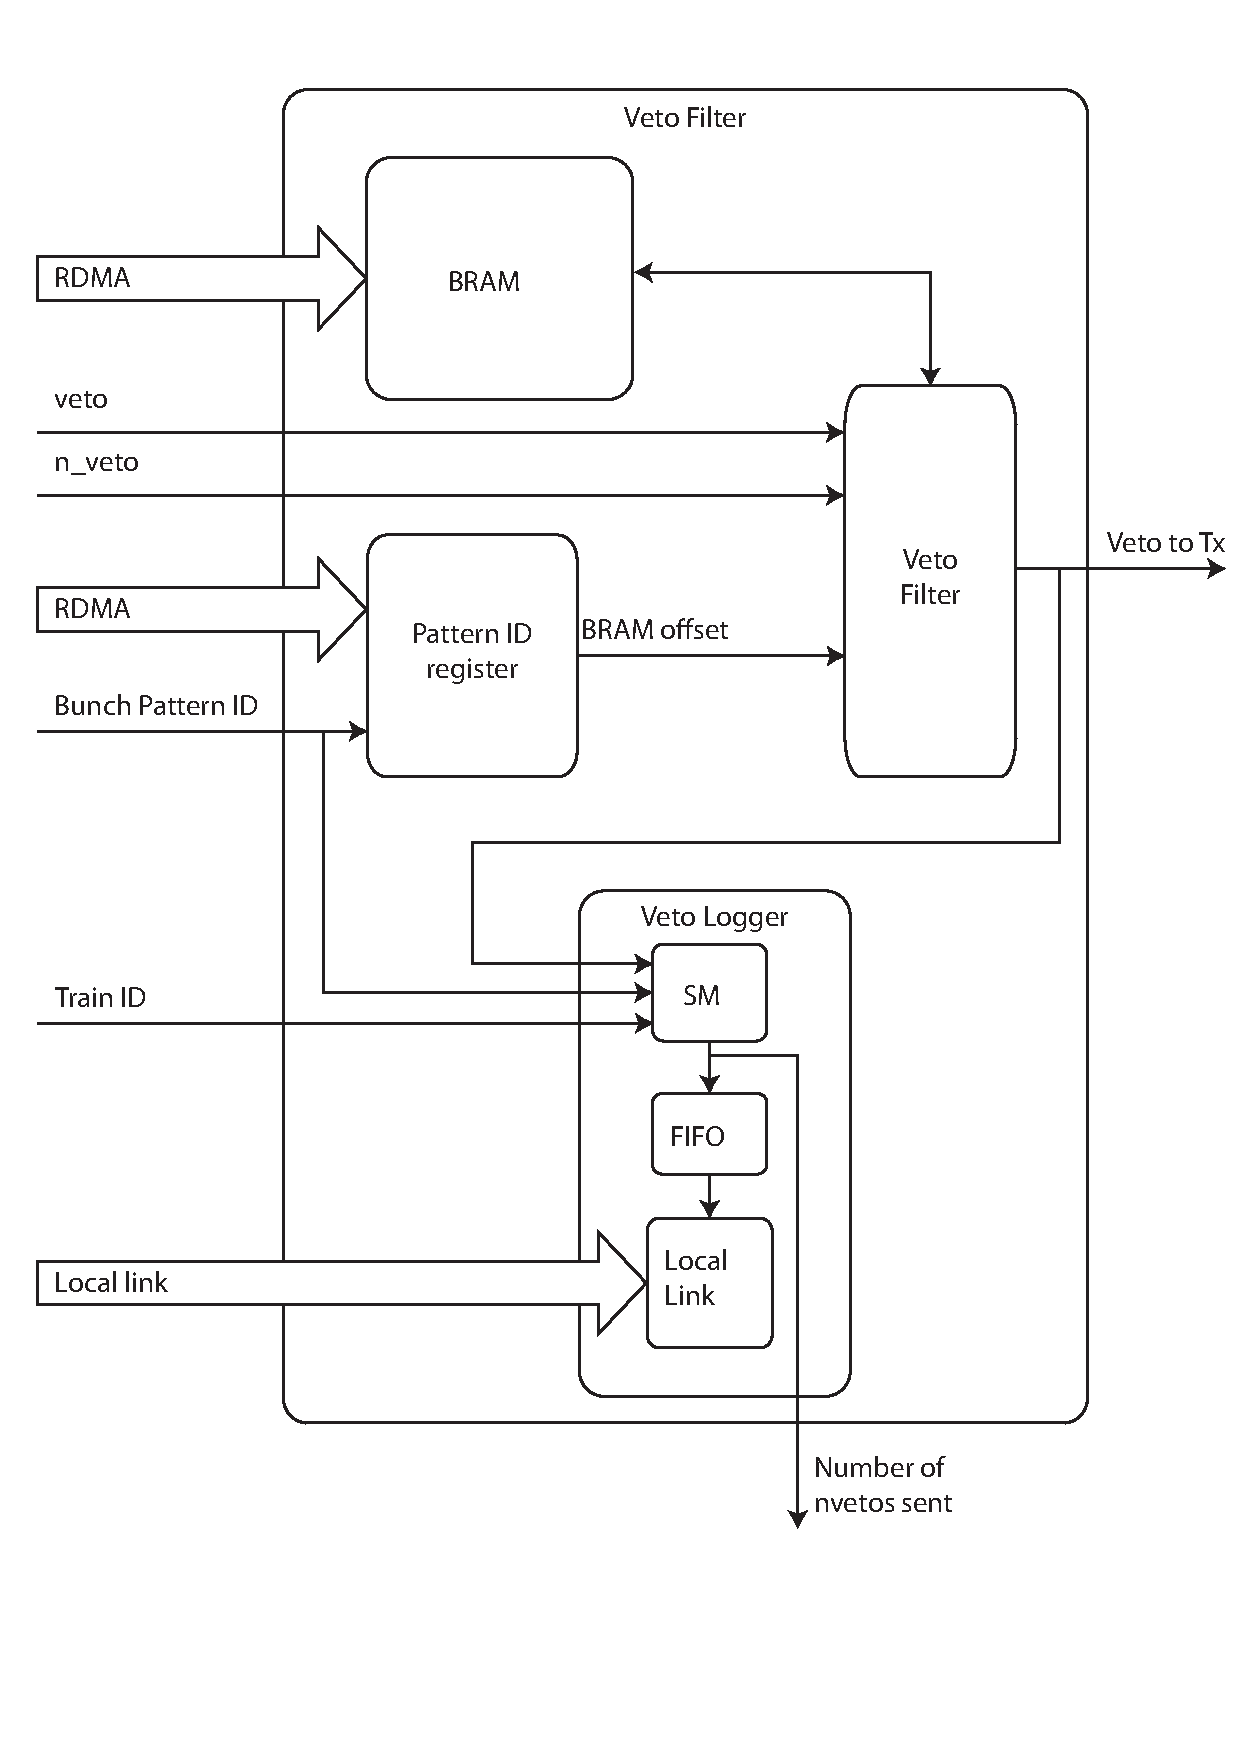
\includegraphics[width=0.7\textwidth]{images/pdfs/veto_filter_block.pdf}
  \caption{Block diagram of the veto filter.}
  \label{fig:veto_filter_entity}
\end{figure}
    
The  1,024\( \times \)32b BRAM is used to store the veto patterns to be combined with the veto signal in order to form the veto decisions. To construct the veto decision and control access into the BRAM a state machine is implementing figure~\ref{fig:veto_filter_flow} was used. The veto decisions are made at the beginning of each word to reduce latency whilst BRAM and state changes are made at the end. The final entity, the pattern ID register, exists to specify the mapping from bunch pattern ID to BRAM offsets.
    
\begin{figure}[htbp]
  \centering
  \includegraphics[width=0.8\textwidth]{images/pdfs/veto_filter_flow.pdf}
  \caption{Flow diagram of the veto filter.}
  \label{fig:veto_filter_flow}
\end{figure}
    
The logging is performed using a simple state machine to feed in words to a 32b in, 256b out first in, first out BRAM (FIFO), this state machine (figure~\ref{fig:veto_logger_flow}) also constructs the LocalLink frame header (the train ID, the bunch ID then `0' padding). The header requires 8 clocks between \texttt{start\_i} being asserted and \texttt{veto\_start}, to be properly formed. The FIFO is a simple First Word Fall Through (FWFT) entity with the optional \texttt{empty} and \texttt{almost\_empty} signals enabled. The read out of the FIFO is performed via a 256b-word LocalLink interface. Once either \texttt{stop\_i} is asserted or \texttt{N\_BUNCHES} have been counted any remaining bits of the 256b word are filled with `1's and the LocalLink's \texttt{src\_rdy} is asserted. 
    
The LocalLink interface is implemented by wrapping the FIFO's 256b \texttt{data\_out} port in some simple logic to make it conform to the local link standard. This mainly involves using \texttt{empty} to monitor the state of the FIFO, \texttt{almost\_empty} as \texttt{eof} and an internal flag from the logging state-machine for the \texttt{sof}. The \texttt{sop} (start-of-payload) signal is not used to differentiate the header from the payload as the entire frame will ultimately form part of the meta-data in the header of the read-out.
    
\begin{figure}[htbp]
  \centering
  \includegraphics[width=0.8\textwidth]{images/pdfs/veto_logger_flow.pdf}
  \caption{Flow diagram for the veto decision logger.}
  \label{fig:veto_logger_flow}
\end{figure}

% subsection veto_implementation (end)
% section veto_filter (end)
%%%%%%%%%%%%%%%%%%%%%%%%%%%%%%%%%%%%%%%%%%%%%%%%%%%
\section{Transmitter} % (fold)
\label{sec:transmitter}
The transmitter entity's main task is to act as the interpreter for the signals received from the CCC, translating them into command sequences that the ASIC can understand and act upon. As has been discussed above there are four signals that need to be translated for the ASIC: \texttt{START}, \texttt{STOP}, \texttt{RESET} and (\texttt{NO-})\texttt{VETO}. The first three command signals all require an arbitrary number of words be sent to the ASIC whilst the veto signals are responded to by one of two words.
    
The transmitter can run in one of two mode: `dynamic veto mode' and `reset mode'. Dynamic veto mode is intended to be the normal mode of operation for XFEL whilst reset mode is intended for static runs with simple veto patterns (e.g.\ for testing). A comparison of the two can be seen in table~\ref{tab:dynamic_vs_reset_mode}. Reset mode is enabled by strobing bit 0 of the main control register (see section~\ref{sub:ctrl_reg} for details). The transmitter also has an optional minor mode called `down-scaler mode' this is primarily for v~1.0 of the ASIC that requires a slower clock during readout. When enabled it uses a multiplier (set by generic) to slow slow the clock, after a set number of cycles normal speed is resumed. 
    
\begin{table}[htbp]
  \begin{center}
    \begin{tabular}{r | X{2.5cm} | X{2.5cm} }
      & \multicolumn{2}{c}{Mode} \\
      & Dynamic-veto & Reset \\
      \hline
      Standalone operation   & \xmark & \cmark \\
      Dynamic veto decisions & \cmark & \xmark \\
      \multirow{4}{*}{Signal response}
      & START  & \multirow{4}{*}{Register flag} \\
      & STOP   & \\
      & RESET  & \\
      & N/VETO & 
    \end{tabular}
  \end{center}
  \caption{Comparison of dynamic veto and reset modes}
  \label{tab:dynamic_vs_reset_mode}
\end{table}

\subsection{Controlling the ASIC} % (fold)
\label{sec:controlling_the_asic}

The LPD ASIC manual~\cite{lpd_manual} specifies the command sequences required for each stage of operation of the ASIC. For the veto commands a simple selection between \texttt{NOP} (veto) and \texttt{TRIGGER\_FLAG\_SET} (no-veto) is required, the other commands have more complex sequence sets that can change based on operation a brief summary will be given here full details can be found in the LPD ASIC manual~\cite{lpd_manual}. 

The standard response to the START command is to set the ASIC in a state ready to write to its memory, this means reseting the write and trigger points and clearing the skip register. Once these commands have been carried out the ASIC will start incrementing the write pointer through the memory locations after additionally starting the trigger pointer the ASIC is ready to write the contents of the pixels when a \texttt{TRIGGER\_FLAG\_SET} (i.e.\ NO-VETO) is received. 

The command sequence for the STOP command is more complex and split over two stages: the pre and post readout sections. To start readout the ASIC is set in a stable mode thus:
\begin{enumerate}
  \item The ASIC is put in power saving mode.
  \item Read out of the data begins.
  \item Disable on-chip resets.
  \item Manually reset the gain, pre-amp, write and trigger pointers.
\end{enumerate}
The data read back consists of one 36b word for each no-veto sent, once all of these have been sent the ASIC is returned to ready mode for the next train:
\begin{enumerate}
  \item Power up the ASIC, i.e.\ return bias currents to full
  \item Re-synchronise the ASIC to the bunch (\( \sim \)4.5~MHz) clock.
  \item Re-enable on chip resets.
  \item Stop read out.
\end{enumerate}
\textbf{NOTE:} the above constitute a basic over view of the STOP process, there are some important considerations with regards to synchronisation of these commands that are beyond the scope of this and covered in full in the LPD ASIC manual~\cite{lpd_manual}.

The ASIC command words have the format:
\begin{align}\label{fmt:asic_format}
  <\text{SYNC }19><\text{X }18<\text{CMD } 17:10><\text{PADDING\_ZEROS } 9:0>
\end{align}
if a word length greater than 20b is being used (e.g.\ 22b, the current default) then the zero-padding is extended as required. The `SYNC' bit is a `1' and `X', by convention, a `0' these are automatically prepended by the state machine. The only exception to this is the 20b command \texttt{SYNC\_RESET} (currently set to be 0x5A5A5) which overrides the above format.

% section controlling_the_asic (end)
\subsection{Interface} % (fold)
\label{sub:tx_interface}
The transmitter has three `sets' of generics: the control register reset values, the flag words (ending in \texttt{\_SIG}) and the down-scaler factor. The register resets set the default value to be written to the assorted registers if \texttt{rst} is asserted. The flag words specify certain command words that the transmitter should scan for in order to flag them for use elsewhere. The \texttt{SYNC\_RESET} flag is intended for use with any entities (e.g.\ the slow command line) that have to be synchronised to the ASIC's bunch clock. The \texttt{READOUT} is intended for use by the read-out entity in order to prepare for read-out. The \texttt{DOWNSCALER\_SIG} is used to begin either the internal (if it's enabled) or an external down-scaler clock. The \texttt{DOWNSCALER\_STOP\_SIG} is only for use by an external source (the internal version counts clocks). The \texttt{DOWNSCALER\_FACTOR} specifies the factor to use for the internal down-scaler e.g.\ a factor of 100 means a scale of 100 fast clock cycles to each slow clock.
    
The in ports to the transmitter are all flags from the receiver; with the standard exception of \texttt{rst} which is the FEM internal signal (cf.\ \texttt{reset} which is the flag from the receiver).
    
The out ports fall into 3 categories: signals to the ASIC (\texttt{ASIC\_in} and \texttt{clk\_in}), flags (marked \texttt{\_sent}) and \texttt{start\_nwords\_o}. The ASIC commands are defined in the specification. The flags have been discussed above with regards to their generic-defined trigger words. The final out port is a wrapper to the value of the \texttt{start\_nwords} register (see section~\ref{sub:tx_registers}) which is used in setting the delay for \texttt{veto\_start}.
    
The two RDMA interfaces are used for access to the command sequence BRAM and the control registers (sections~\ref{sub:tx_bram} and \ref{sub:tx_registers} respectively).
    
\begin{table}[htbp]
  \begin{center}
    \begin{tabulary}{\textwidth}{l | c | c | L}
      Name & Direction & Type & Description \\
      \hline
      REG\_RESET\_(9:0)     & & slv (31:0) &  Register resets (0-9), see section~\ref{sub:tx_registers}. \\
      SYNC\_RESET\_SIG      & & slv (31:0) & Flag that the \texttt{SYNC\_RESET} command has been sent.                 \\
      READOUT\_SIG          & & slv (31:0) & Flag that the \texttt{READOUT} command has been sent.               \\
      DOWNSCALE\_SIG        & & slv (31:0) & Flag to start the down-scaler (either internal or external).\\
      DOWNSCALER\_STOP\_SIG & & slv (31:0) & Flag to stop the down-scaler.                               \\
      DOWNSCALE\_FACTOR     & \multirow{-6}{*}[11.5pt]{Generic} % Avoids extra newline at top
      % DOWNSCALE\_FACTOR     & \multirow{-16}{*}[11.5pt]{Generic} % Avoids extra newline at top
                              & integer    & Factor for the internal down-scaler, default: 100.          \\
      \hline
      clk   & \multirow{6}{*}{in} 
               & sl & The CCC clock.          \\
      rst   &  & sl & FEE reset.              \\
      start &  & sl & From the receiver entity.\\
      stop  &  & sl & \dittostraight          \\
      reset &  & sl & \dittostraight          \\
      veto  &  & sl & From the veto filter.   \\
      \hline
      % asic\_in                & \multirow{7}{*}[-28.75pt]{out}
      asic\_in                & \multirow{7}{*}{out}
                                 & sl                & Fast serial commands to the ASIC.  \\
      clk\_in                 &  & sl                & Clock to the ASIC.  \\
      readout\_sent           &  & sl                & Readout flag (for ASIC receiver entity).  \\
      rsync\_sent             &  & sl                & \texttt{SYNC\_RESET} flag (for slow control entity).  \\
      downscaler\_start\_sent &  & sl                & Downscaler start flag.  \\
      downscaler\_stop\_sent  &  & sl                & Downscaler stop flag.  \\
      start\_nwords\_o        &  & slv (31:0) & Number of words used for `START' to set veto\_start delay.\\
      \hline
      bram\_rdma & \multirow{2}{*}[-17.25pt]{Interface} 
      & RDMA & Interface to the ASIC command word BRAM. Mask: 0x000003FF. \\
      ctrl\_rdma & & RDMA & Interface to the control register. Mask: 0x0000000F. \\
    \end{tabulary}
  \end{center}
  \caption{Interface for the transmitter.}
  \label{tab:tx_interface}
\end{table}
  
% subsection tx_interface (end)
\subsection{Registers} % (fold)
\label{sub:tx_registers}
There are two externally accessible sets of registers in the transmitter entity, a control register and the command BRAM both are accessed via RDMA (see appendix~\ref{app:rdma_interface}). The control registers direct the flow of the state machine whilst the BRAM stores the instruction sets to be sent to the ASIC. There are 3 commands that the BRAM has instruction sets for: \texttt{START}, \texttt{STOP} and \texttt{RESET}. Obviously these are normally received via the receiver module but the \texttt{RESET} command can also be sent using a toggle in the control register.
\subsubsection{Control register} % (fold)
\label{sub:ctrl_reg}
The control register specifies 10 registers:
\begin{description}
  \item[1] The general state-machine control register that toggles various modes (i.e. whether to use the down-scaler module and manual \texttt{RESET}) as well as how many bits to send downscaled if that mode is enabled.
  \item[2-7] three pairs of registers that store the number of words (shortened to `nw') and offsets for the 3 different instruction sets (i.e. one \emph{-nw} and one \emph{-offset} for each of \texttt{START}, \texttt{STOP} and \texttt{RESET}).
  \item[8] The word to be sent in case of a veto.
  \item[9] The word to be sent in case of a no-veto.
  \item[10] The status register, indicates what state the state-machine is in.
\end{description}
default values and addresses are given in table~\ref{tab:ctrl_reg_default}.
    
The state-machine control register takes values of the following format:
\begin{align} \label{fmt:control_reg}
  <\text{DOWNSCALER\_ENABLE } 32>\ldots<\text{DOWNSCALER\_BITS } 20:5>\ldots<\text{RESET\_MODE\_EN } 0>
\end{align}
\texttt{reset\_mode\_en} is a flag to manually start the state-machine in reset mode i.e. \texttt{reset\_nwords} worth of commands from \texttt{reset\_offset} in the BRAM will be sent. This mode can be used instead of dynamically determining the veto to be sent in a `fire and forget' manner.

\textbf{DOWNSCALER\_ENABLE} indicates that the internal down-scaler should be used to send the next \textbf{DOWNSCALER\_BITS}, this means that the maximum number of bits that can be sent at the down-scaled rate is \(2^{16} - 1\), i.e. 65,536 or 2,978\(\times\)22b words. Obviously if down-scaling is being handled by an external clock this restriction doesn't apply.

The BRAM offsets and command sequence lengths (\emph{-offset} and \emph{-nw} registers respectively) have maximum values determined by the size of the BRAM i.e.\ 1,024. These values are set using the LSB of the word i.e.\ 9 downto 0. Obviously setting an \emph{-offset} to 1,024 will result in only 1 word and unless the corresponding \emph{-nw} is set to 1 this will result in an address overflow and undefined behaviour. By the same token setting an \emph{-nw} register to 1,024 is allowed but will mean that any other commands to be sent must be either specified as subsets of this command sequence or not used.\footnote{This could be useful if using the reset-mode or in dynamic mode if \texttt{RESET} is not expected to be used.}
    
The veto/no-veto registers specify the appropriate word to send when in dynamic-veto mode, the defaults are \texttt{NOP} and \texttt{TRIGGER\_FLAG\_SET} respectively. When run in this way the state-machine progresses START\(\rightarrow\)vetoes\(\rightarrow\)STOP with vetoes being determined by the veto filter.
      
The status register is a read only register that logs which state the state-machine is in and has the following format:
\begin{align} \label{fmt:status_reg}
  <\text{state\_machine\_enabled } 31>\ldots<\text{RESET } 3> <\text{STOP } 2> <\text{DYNAMIC\_VETO } 1> <\text{START } 0>
\end{align}
	  
\begin{table}[htbp]
  \begin{center}
    \begin{tabular}{c|c | c |c}
      Address & Description             & Reset generic      & Default value  \\
      \hline                    
      0x1     & SM-Control              & CTRL\_REG\_RESET   & 0x00000000     \\ 
      0x2     & Start: offset           & START\_OFF\_RESET  & 0x00000000     \\  
      0x3     & Start: number of words  & START\_NW\_RESET   & 0x00000006     \\ 
      0x4     & Stop: offset            & STOP\_OFF\_RESET   & 0x00000006     \\ 
      0x5     & Stop: number of words   & STOP\_NW\_RESET    & 0x00000007     \\ 
      0x6     & Reset: offset           & RESET\_OFF\_RESET  & 0x0000000D     \\ 
      0x7     & Reset: number of words  & RESET\_NW\_RESET   & 0x0000000F     \\ 
      0x8     & Veto word               & VETO\_WORD\_RESET  & 0x00210000     \\ 
      0x9     & No-veto word            & NVETO\_WORD\_RESET & 0x00200000     \\ 
      0xA     & Status                  & n/a                & 0x00000000     \\ 
    \end{tabular}
  \end{center}
  \caption{Control register layout. With the exception of the status register the reset values of each register can be changed by setting the appropriate reset-generic, these values only take affect when the \texttt{rst} line is asserted \emph{not} when the \texttt{RESET} signal is received.}
  \label{tab:ctrl_reg_default}
\end{table}

% subsubsection control_regsiter (end)
\subsubsection{Instruction set BRAM} % (fold)
\label{sub:tx_bram}
The BRAM used to store the instruction sets is 1,024\(\times\)32b words. Words not defined by the ASIC are ignored so internal flag triggers (e.g. for \texttt{DOWNSCALER\_START}) need not be defined ASIC commands.

The BRAM expects words to have the format:
\begin{align}\label{fmt:tx_bram}
  <\text{N\_NOPS } 31:\text{WORD\_LENGTH }><\text{COMMAND } (\text{WORD\_LENGTH} - 1):0>
\end{align}
The COMMAND is expected to be correctly padded e.g.\ if 22b words are being used for a normal command the last 12b should be `0'. The SYNC bit doesn't need to be set. N\_NOPS indicates how many \texttt{NOP} commands should follow the COMMAND, a NOP is pre-defined to be a SYNC-bit followed by the appropriate number of 0's. It is important to note that NOPs contribute to the number of words sent for any state and a \texttt{NOP} sent as a member of N\_NOPS must not be the final command.

\textbf{Example:} if, for the \texttt{START}-sequence and using 22b words, \texttt{POWER\_UP} (0x02\footnote{see table~\ref{tab:asic_command_words}}) followed by 4 NOPS is to be sent then the first two locations in BRAM could be set to `0x00C08000' and `0x00000000'. 0x00C specifies 3 NOPS (\(\text{0xC}<<2 = 0x3\)\footnote{Where `\(<<\)' is a left-shift, the \( <<2 \) is account for the 2~MSB of the command.}) and 0x08000 is the command (\(\text(0x02) << 22 \)) with the appropriate padding. The final entry of 0x00000000 is the 4\(^{\text{th}}\) NOP; its SYNC bit will be automatically set.
% subsubsection tx_bram (end)
% subsection tx_registers (end)
\subsection{Implementation} % (fold)
\label{sub:tx_implementation}

In order to implement the state machine two concurrent machines are used: the shift-block serialises and inspects command sequences; and the state-machine that determines when to change state and which command sequences to use. Previously, these responsibilities were split across multiple entities but to simplify state sharing and meet the latency requirements they were merged into a single entity. Figure~\ref{fig:tx_entity} shows a entity diagram of the transmitter, both the shift-block and state-machine are within the state-machine entity.
    
\begin{figure}[htbp]
  \centering
  \includegraphics[width=0.8\textwidth]{images/pdfs/tx_block.pdf}
  \caption{Block diagram of the transmitter.}
  \label{fig:tx_entity}
\end{figure}
        
The shift-entity primarily acts as a smart shift register to serialise the command words being sent to the ASIC. It has two secondary functions that require inspection of the commands being serialised: flagging and setting sync-bits. Some of the other components of the FEM require knowledge of when certain command words are sent for their own functionality (e.g. the slow command needs to know when \texttt{SYNC\_RESET} is sent). To do this when a word is loaded from the BRAM (and only from the BRAM) it is compared to the 4 pre-set words given in table~\ref{tab:shift_entity_flags}, if it matches one then the appropriate flag is set. These words are tested sequentially, in the order given in the table, so if a word matches multiple triggers only the flag corresponding to the first match will be set. The flag words are set via generics and are not expected to change, flags do not have to be valid ASIC words although the ASIC's response to unknown commands is undefined and should be confirmed prior to use. At the same time as checking for flags the first two bits of each word are set appropriately: for \texttt{SYNC\_RESET} they are set to 0b01 and all other words 0b10 as specified in \cite{lpd_manual}. These sync-bits are not included in tests for flags. The shift-entity's functionality for the different states are given in table~\ref{tab:shift_entity_behaviour}, the different states are described below.

\begin{table}[htbp]
  \begin{center}
    \begin{tabular}{c|c|l}
      Flag             & Default    & Notes \\
      \hline
      rsync             & 0x00069694 & Used to keep the slow command line synced to the ASIC.   \\
      readout           & 0x00044400 & Used to alert the readout receiver entity of input.       \\
      down-scaler start & 0x00044000 & Moving to the slower clock (either internal or external).\\
      down-scaler stop  & 0x00055000 & Stop using the slow clock (external only).               \\
    \end{tabular}
  \end{center}
  \caption{Flag information, these are command words that the shift-entity looks for and will flag along. Default values are for 22b words, see section~\ref{sub:tx_bram} for more details. When looking for flags the sync bits (the first two bits) are ignored so do not need to be set.}
  \label{tab:shift_entity_flags}
\end{table}
    
\begin{table}[htbp]
  \begin{center}
    \begin{threeparttable}
      \begin{tabular}{r|c|c|l}
        State & Flags enabled & Sync-bit set & Command source                        \\
        \hline                                                                       
        IDLE  &    \xmark     &    \xmark    & n/a                                   \\
        NOPS  &    \xmark     &    \cmark    & State machine, command = 0x0\tnote{1}.\\
        VETO  &    \xmark     &    \cmark    & State machine, either veto or no-veto.\\
        START &    \cmark     &    \cmark    & BRAM: START command sequence.         \\
        STOP  &    \cmark     &    \cmark    & BRAM: STOP command sequence.          \\
        RESET &    \cmark     &    \cmark    & BRAM: RESET command sequence.         \\
      \end{tabular}
      \begin{tablenotes}
        \scriptsize
        \item[1] i.e. 0x200000 is the full 22b command, including sync-bit.
      \end{tablenotes}
      \caption{Description of the shift-entity's behaviour depending on state.}
    \end{threeparttable}
  \end{center}
  \label{tab:shift_entity_behaviour}
\end{table}
    
The second process, the state-machine, is mainly concerned with maintaining position within each command sequence, changing state and controlling the BRAM. Figure~\ref{fig:tx_sm_flow} shows the relationship between the different states and the causes for state changes. Meanwhile figure~\ref{fig:tx_sm_bram_control_flow} shows how access to the BRAM is determined. During state changes the source of the next word is set according to the sources in table~\ref{tab:shift_entity_behaviour}, obviously this change occurs before the actual state changes. It's important to note that, as discussed in section~\ref{sub:tx_bram} the final word of any sequence should sent from the NOP state as control returns to the origin state, e.g. `START\( \rightarrow \)NOPS\( \rightarrow \)VETO' is not permitted, if the final word is required to be a \texttt{NOP} then this should be set as a unique BRAM entry. 
    
\begin{figure}[htbp]
  \centering
  \includegraphics[height=0.8\textheight]{images/pdfs/tx_sm_flow.pdf}
  \caption{Schematic of the control flow in the transmitter entity.}
  \label{fig:tx_sm_flow}
\end{figure}
  
\begin{figure}[htbp]
  \centering
  \includegraphics[width=0.7\textwidth]{images/pdfs/tx_sm_bram_control_flow.pdf}
  \caption{General control logic flow for START, STOP and RESET states.}
  \label{fig:tx_sm_bram_control_flow}
\end{figure}
% subsection tx_implementation (end)
% section transmitter (end)
%%%%%%%%%%%%%%%%%%%%%%%%%%%%%%%%%%%%%%%%%%%%%%%%%%%

% chapter implementation (end)
%%%%%%%%%%%%%%%%%%%%%%%%%%%%%%%%%%%%%%%%%%%%%%%%%%%
\chapter{Testing} % (fold)
\label{cha:testing}
This chapter is concerned with the testing regime used on the design. It is split into two sections, first the methodology is discussed and then the results. The aim of testing is to ensure that firstly the design meets the requirements (see chapter~\ref{cha:design}) and secondly that the limitations of the system are understood.
\section{Methodology} % (fold)
\label{sec:methodology}
The methodology used for testing was to iterate rapidly, working from smaller to larger entities and limiting changes to the outer most entity being tested, changes made in sub-entities restarted the processes from that entity to confirm functionality at each level. 

In order to test the designs `test benches' were written. A test bench is a entity that wraps another, the Unit Under Test (UUT), and generates test inputs UUT so its behaviour can be checked. These simulated inputs can be single signals, words or clocks. The UUT and test bench are then simulated and run using a program called, in this case called `iSim', which gives complete control over the system, this means that the response of sub-units can be tested as well as top-level entities. iSim generates an output that is similar to an oscilloscope view with green traces representing boolean values (`1' or `0') and other colours for the other std\_logic values (e.g.\ orange corresponds to `U'). 

% section methodology (end)
\section{Results} % (fold)
\label{sec:results}
While each individual entity was tested, for brevity only the top level tests are included here as they describe the full functionality of the firmware. There are six tests that were run: a simple dynamic run (\texttt{START}\(\rightarrow\)\texttt{NO-VETO}\(\rightarrow\)\texttt{STOP}); veto/no-veto state changes; response to reset command; stop with down-scaler (a requirement for the v~1.0 ASIC); RDMA interface test; and a LocalLink interface test.

For all of these tests there were a couple of pass requirements:
\begin{itemize}
  \item Correct command to response matching.
  \item Synchronicity with the bunch clock
  \item Fixed latency between commands and responses. 
  \item Correct state changes.
\end{itemize}

In the following diagrams the green portions correspond to the iSim traces, the red and blue lines have been added afterwards and indicate chains of causation and serialised command words respectively, the larger yellow dashed lines were also added and indicate bunch trains synchronised to the \texttt{clk\_to\_asic}. On the left hand side are the signal names as used in the design, note that these may not always match the names given in the previous implementation sections.

In all of these tests the clock speed was set to 100~MHz.

\subsection{Start, no-veto, stop} % (fold)
\label{sec:start_no_veto_stop}
Figure~\ref{fig:isim_start-veto-stop} shows a very simple dynamic sequence with a single no-veto word being sent prior to stopping. The top six lines show the \texttt{clk}, \texttt{rst} signals; the transmitter's state (\texttt{current\_state}); the simulated input from the CCC (\texttt{cmd} and \texttt{veto}); and the output to the ASIC (\texttt{cmd\_to\_asic}).

After the \texttt{START} signal is received from the CCC the appropriate flag (\texttt{start\_from\_rx}) is set, followed by the delayed flag (\texttt{start\_delayed}) to the transmitter, which starts sending the appropriate command set.\footnote{The first word to the ASIC is \texttt{RSYNC} so begins with a `0' rather than `1'.} The delayed flag then forms the \texttt{log\_start} and \texttt{veto\_start} signals that indicate when to log the header information and start logging vetoes respectively. Meanwhile the \texttt{NO-VETO} signal is received and combined with the \texttt{veto\_start} to form flag that the transmitter should send a \texttt{TRIGGER\_FLAG\_SET}. Finally the \texttt{STOP} signal is received, triggering the stop sequence and ultimately a return to IDLE (not shown).

Based on the general requirements it's clear that the correct responses are being sent (and hence the state-changes are occurring as required), the commands are synchronised with the bunch clock and the latency is as required: 6~clocks for commands and 7 for vetoes (the extra length for vetoes is due to the three rather than four bit command).

\begin{sidewaysfigure}[H]
    \centering
    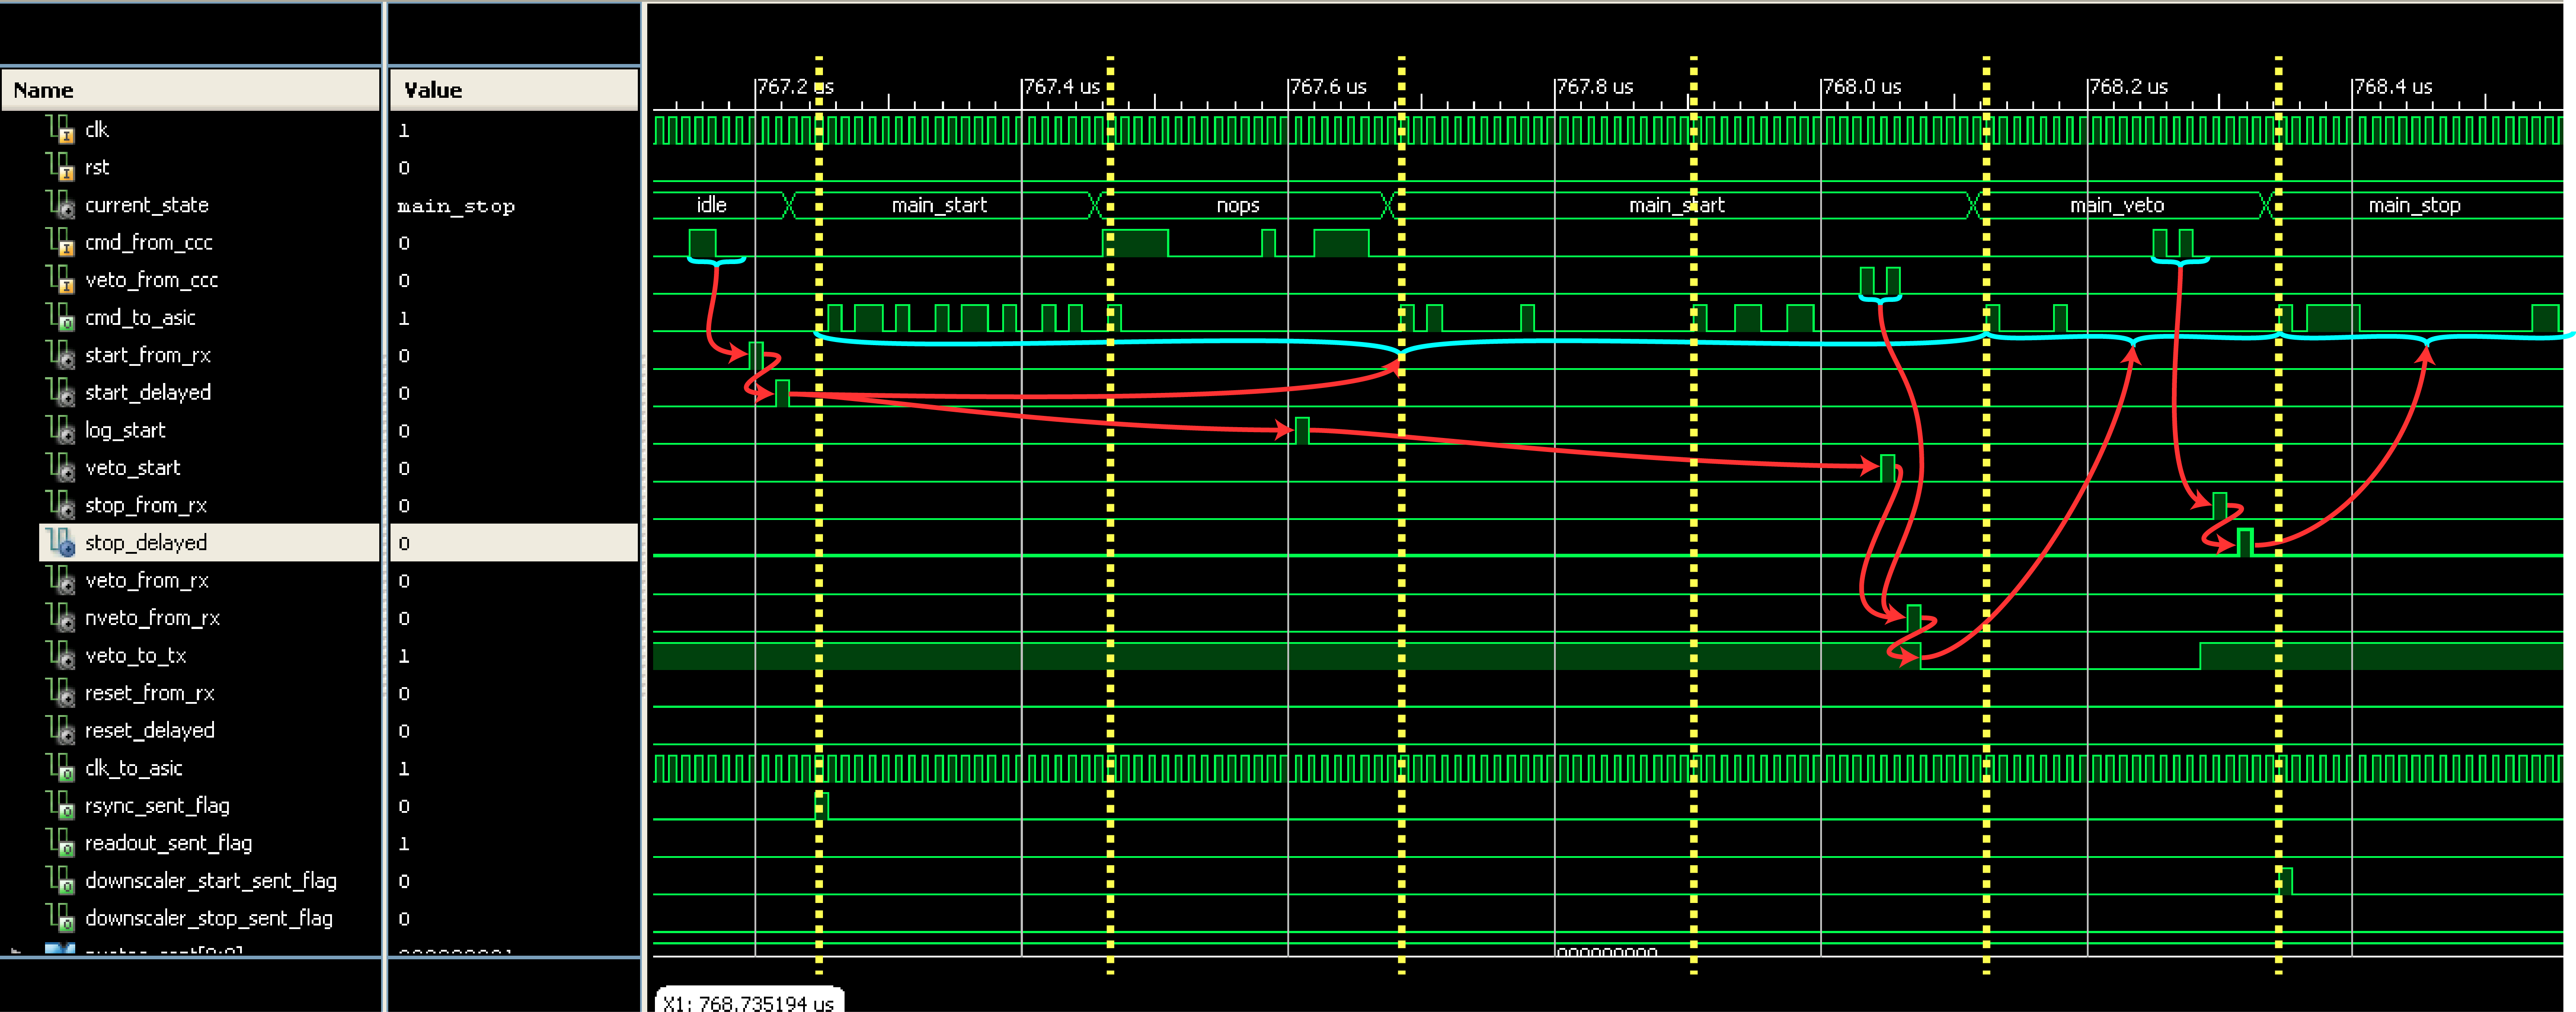
\includegraphics[width=\textwidth]{images/isim/edited/start-veto-stop.png}
    \caption{A \texttt{START}, \texttt{NO-VETO}, \texttt{STOP} sequence with a single \texttt{NO-VETO} prior to the stop signal. The blue braces indicate either input/output word sequences whilst the red lines show logical sequences.}
    \label{fig:isim_start-veto-stop}
\end{sidewaysfigure}

% subsection start_no_veto_stop (end)
\clearpage
\subsection{Veto/No-veto} % (fold)
\label{sec:veto_no_veto}
Figure~\ref{fig:isim_veto_no_veto} shows the dynamic veto mode in operation, 3 vetoes followed by 6 no-vetoes. The main lines to note are between \texttt{veto\_from\_ccc} and \texttt{veto\_to\_tx}. The general operation is: first the signal is received and flagged (on either of the two lines, \texttt{veto\_from\_rx} and \texttt{nveto\_from\_rx}), the decision is made by the veto-filter (\texttt{veto\_to\_tx}) and the response sent to the ASIC. The different responses can be seen in the single \texttt{NOP} for \texttt{VETO}s whilst the \texttt{TRIGGER\_FLAG\_SET} (0x10) is sent for \texttt{NO-VETO}. 

\begin{sidewaysfigure}[H]
  \centering
  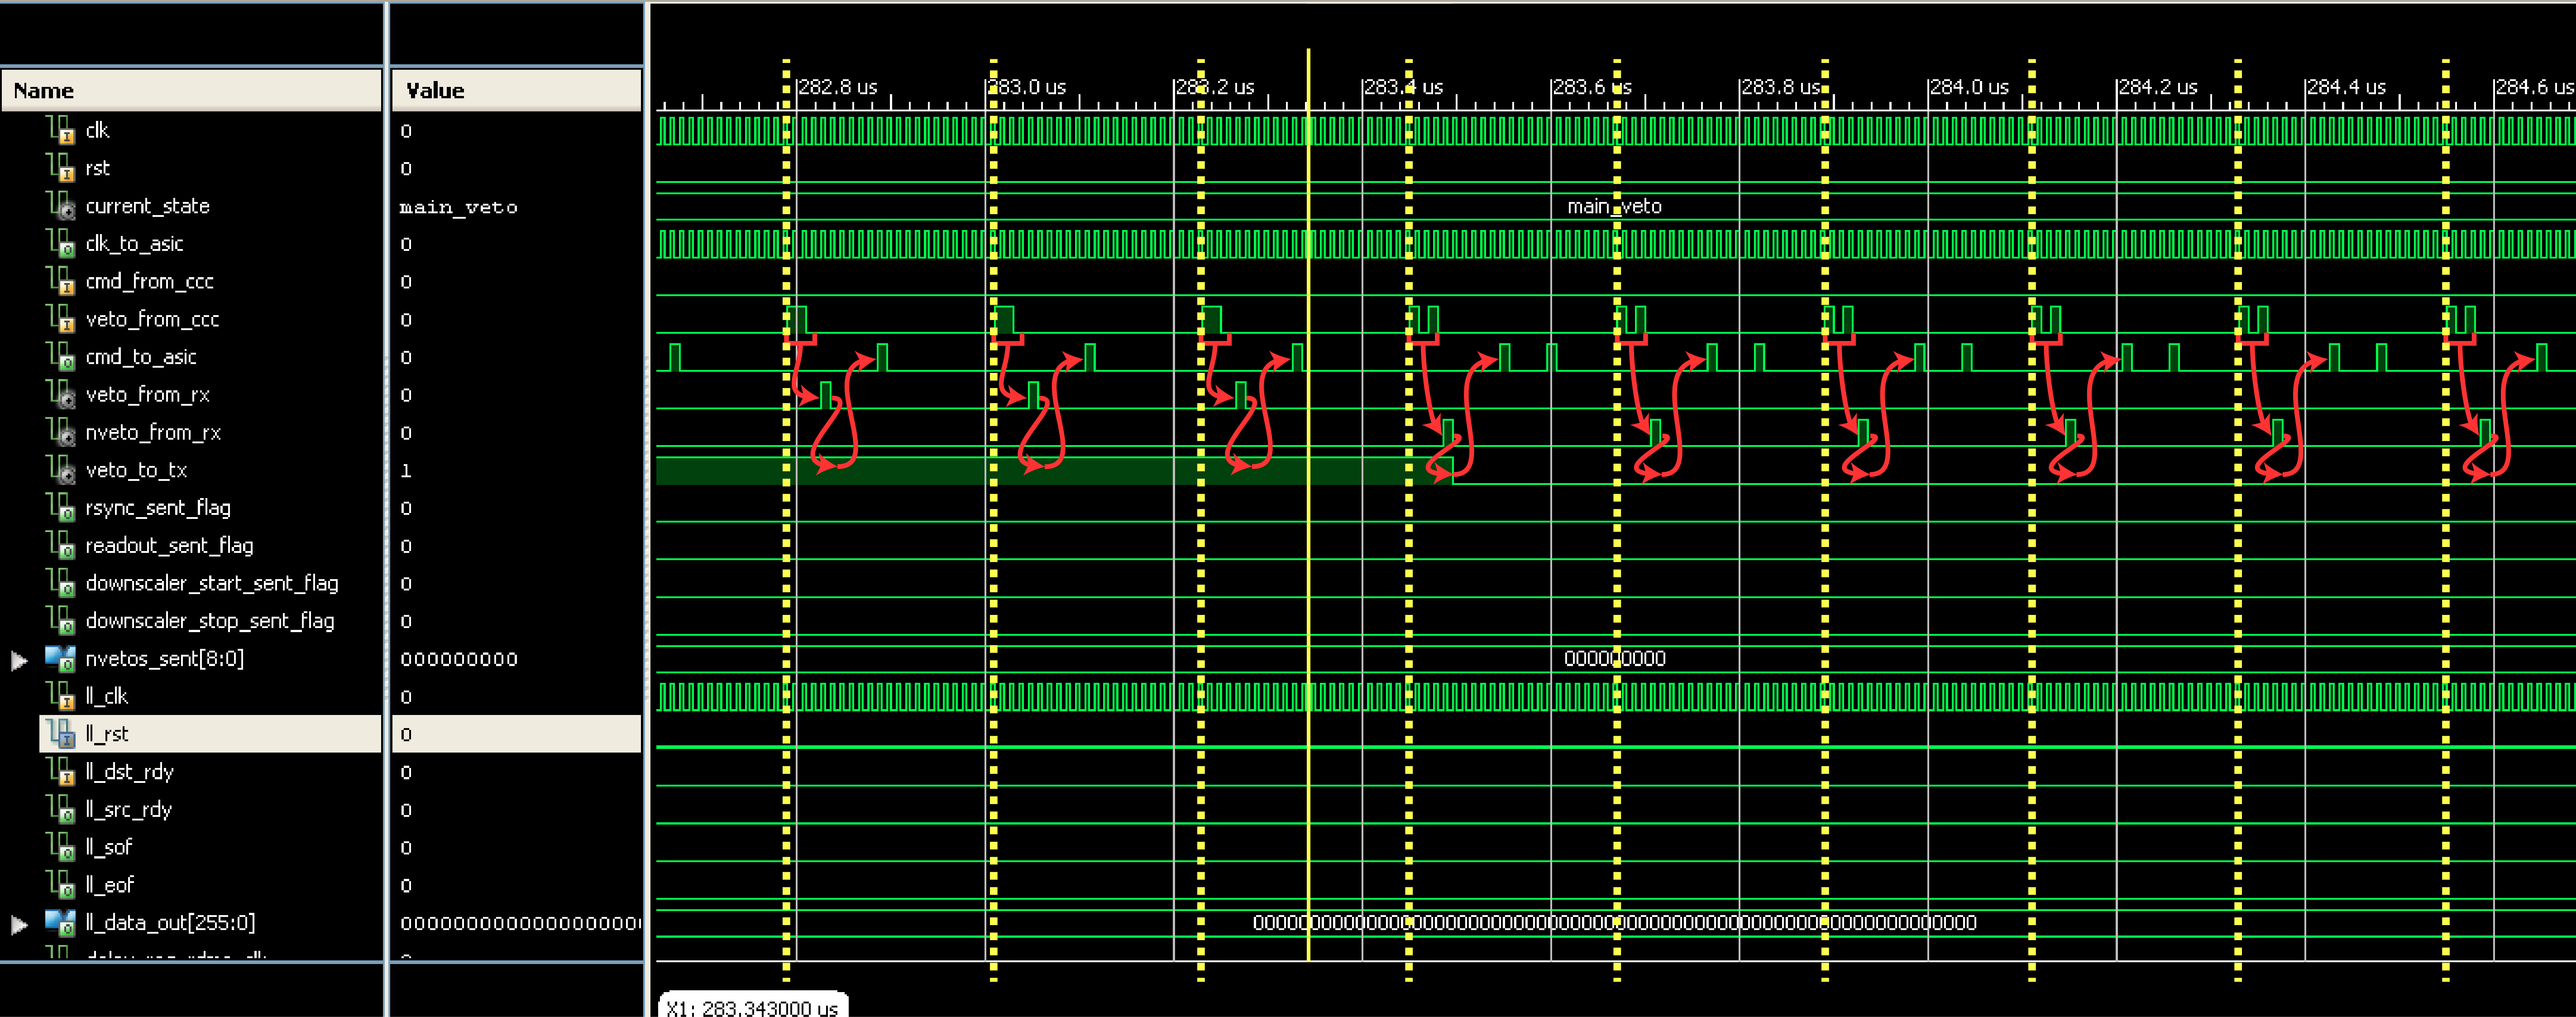
\includegraphics[width=\textwidth]{images/isim/edited/veto_no_veto.png}
  \caption{A selection of vetos/no-vetos.}
  \label{fig:isim_veto_no_veto}
\end{sidewaysfigure}
% subsection veto_no_veto (end)
\clearpage
\subsection{Reset Command} % (fold)
\label{sec:reset_command}
Figure~\ref{fig:isim_reset_cmd} shows the reset sequence being sent in response to the \texttt{RESET} command from the CCC, first the word arrives, then we see the delayed signal from the receiver and then the thee words sent to the ASIC. The first word of the \texttt{RESET} command sequence is a \texttt{RSYNC} so the \texttt{rsync\_sent\_flag} is asserted also it contains a \texttt{NOP} command so the appropriate state change occurs and a single \texttt{NOP} is sent. Figure~\ref{fig:isim_reset_rdma} shows the same process being triggered via the control register which is set via RDMA, i.e.\ the `reset-mode'.
\begin{sidewaysfigure}[H]
  \centering
  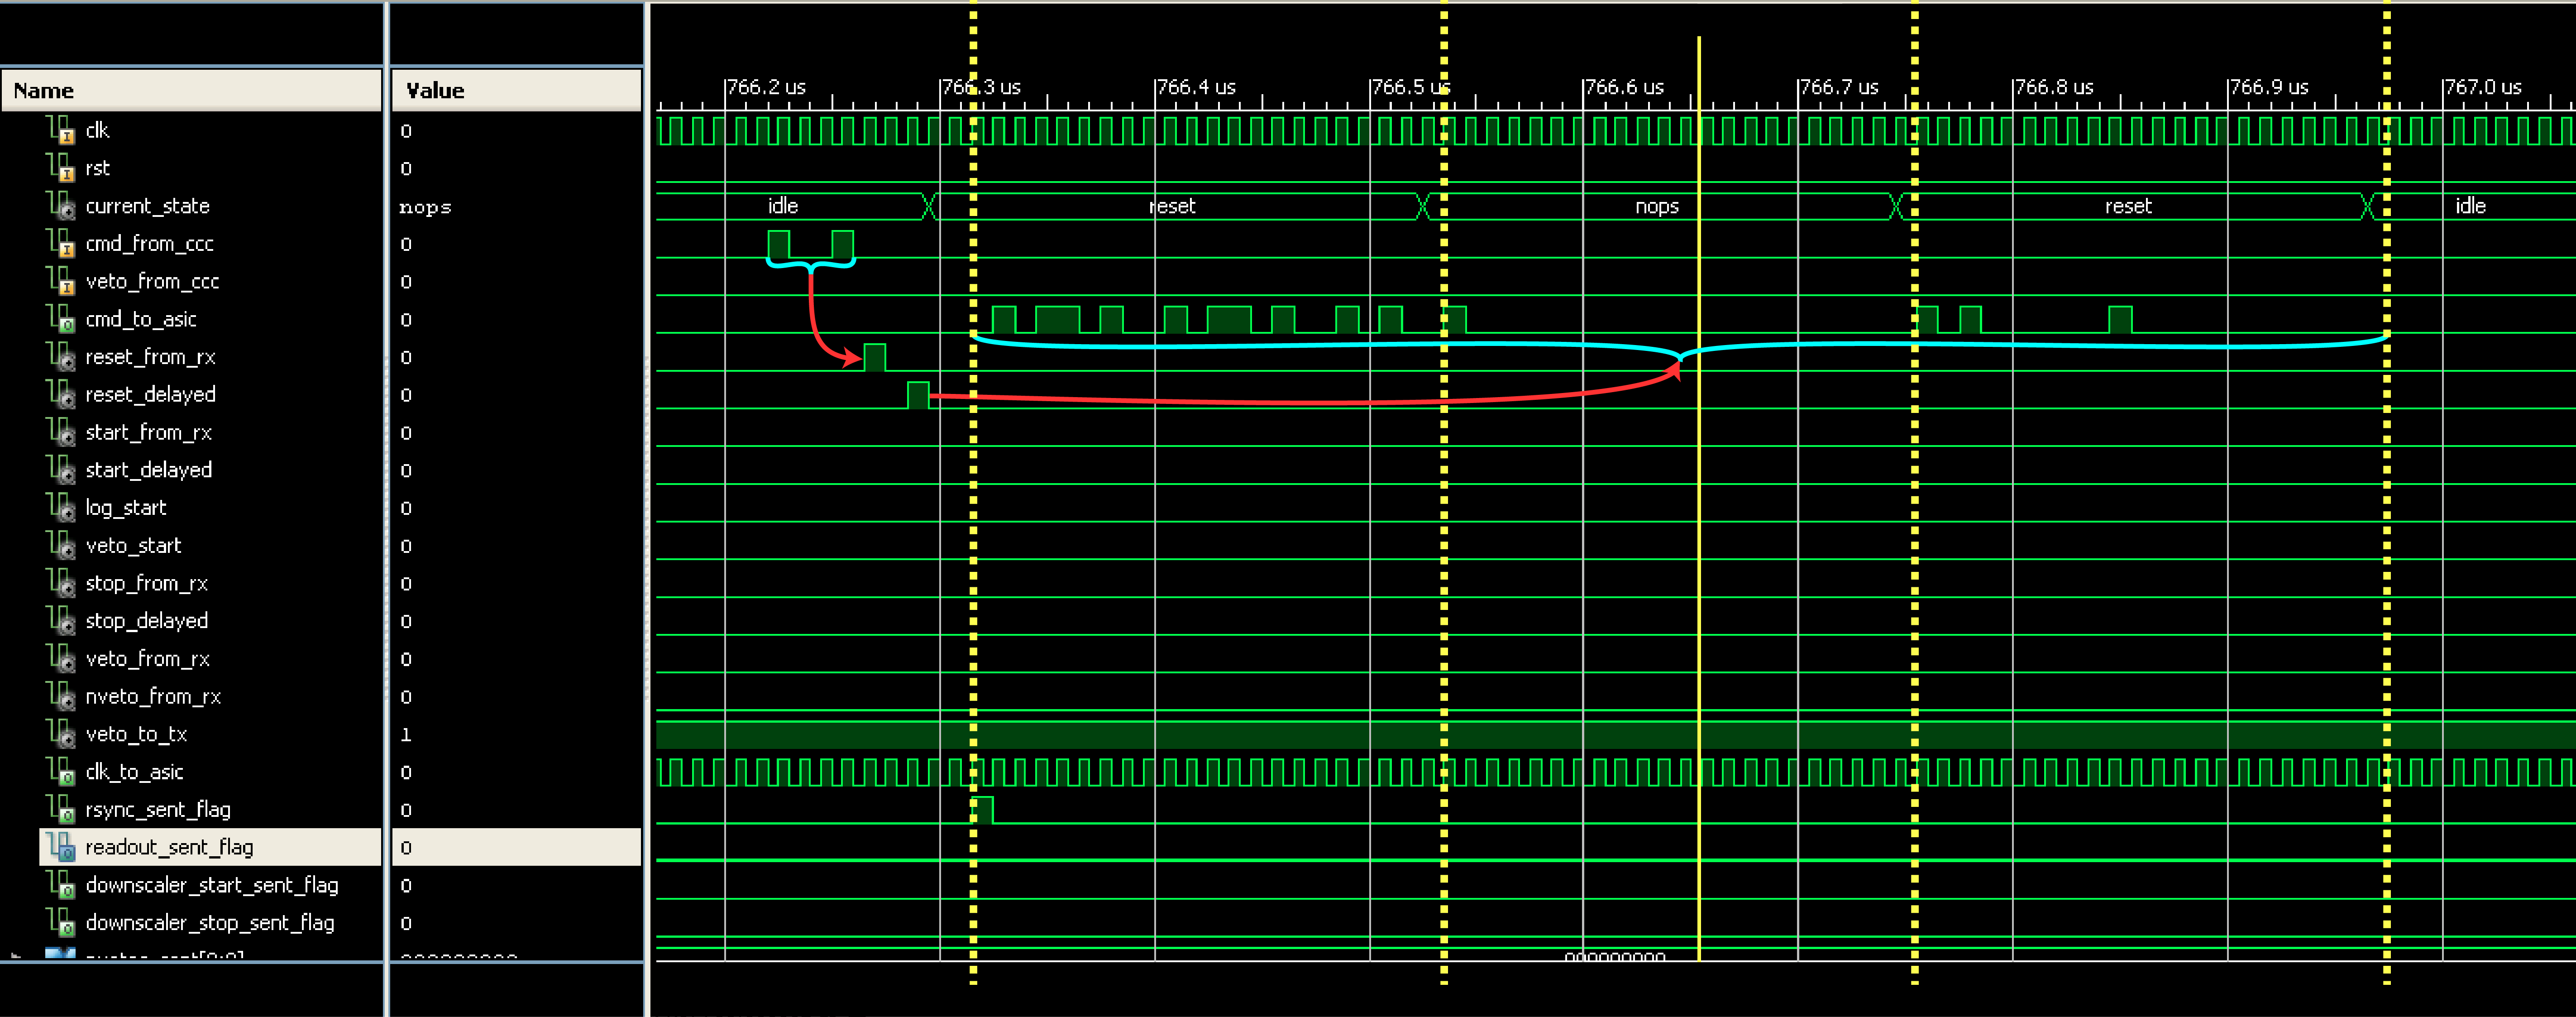
\includegraphics[width=\textwidth]{images/isim/edited/reset_cmd.png}
  \caption{The reset sequence being triggered by the cmd line from the CCC.}
  \label{fig:isim_reset_cmd}
\end{sidewaysfigure}
\begin{sidewaysfigure}[H]
  \centering
  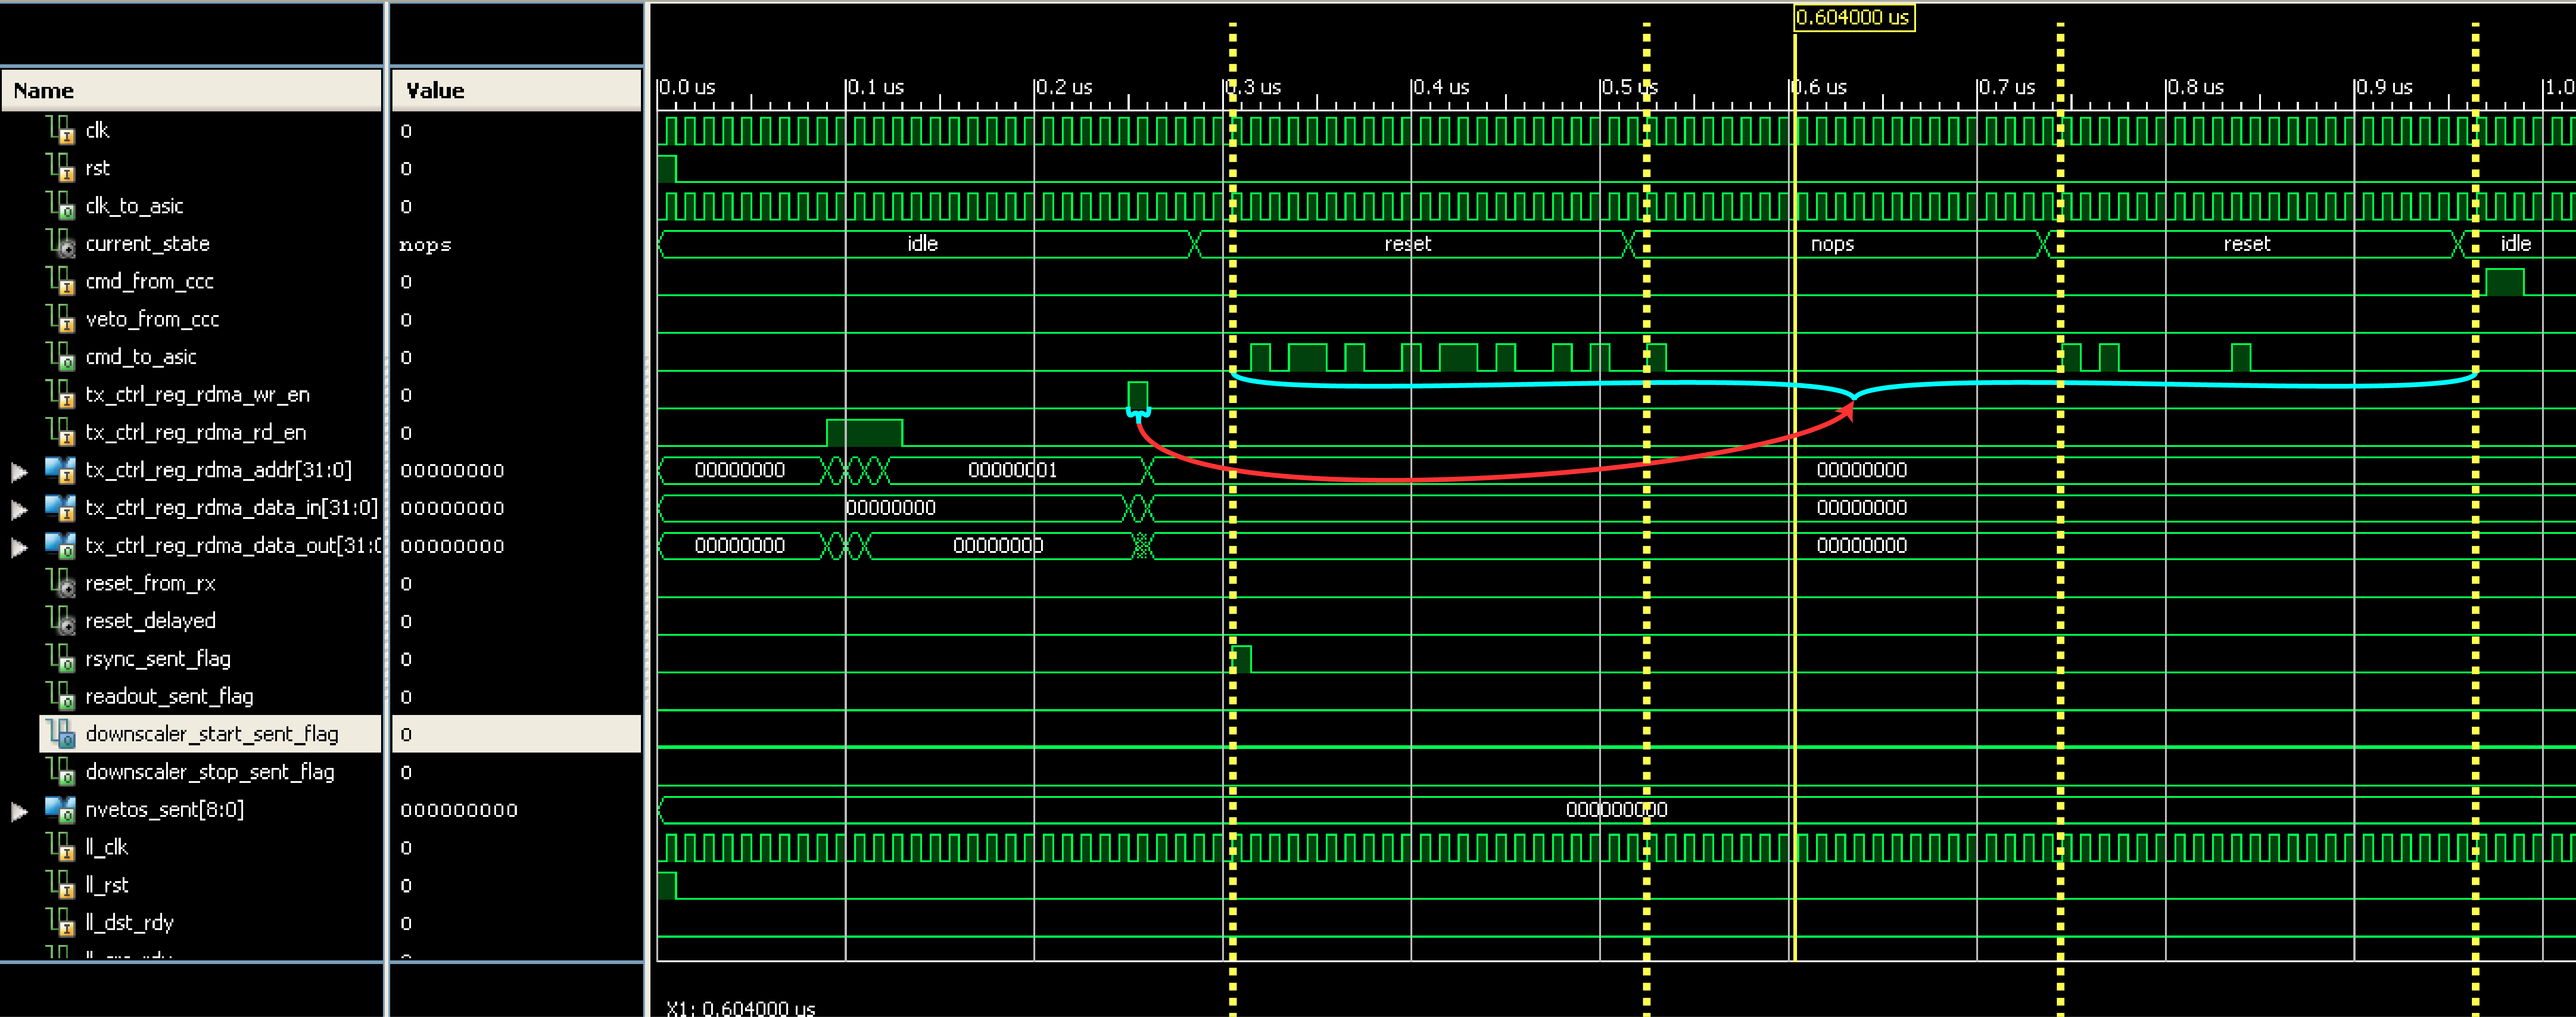
\includegraphics[width=\textwidth]{images/isim/edited/reset_rdma.png}
  \caption{The reset sequence being triggered via the control register.}
  \label{fig:isim_reset_rdma}
\end{sidewaysfigure}
% subsection reset_command (end)
\clearpage
\subsection{Stop with down-scaler} % (fold)
\label{sec:stop_downscaler}
For this test the operation of the down-scaler for the v~1.0 ASIC checked. Prior to the yellow-dashed line in figure~\ref{fig:isim_stop-downscaler} the \texttt{clk\_to\_asic} is running at 100~MHz, after it runs at 1~MHz. The order of events is more clearly show in the close up, figure~\ref{fig:isim_stop-downscaler-zoom}, which corresponds to the region between the dashed and solid lines in figure~\ref{fig:isim_stop-downscaler}. Once the \texttt{STOP} command is received the first word, the down-scaler trigger, is sent to the ASIC, once this is sent the next word (in this case \texttt{READ\_OUT\_DATA}) is sent at the selected speed. Note that the \texttt{READ\_OUT\_DATA} flag is set and held for one clock at the down-scaled speed.

\begin{sidewaysfigure}[H]
  \centering
  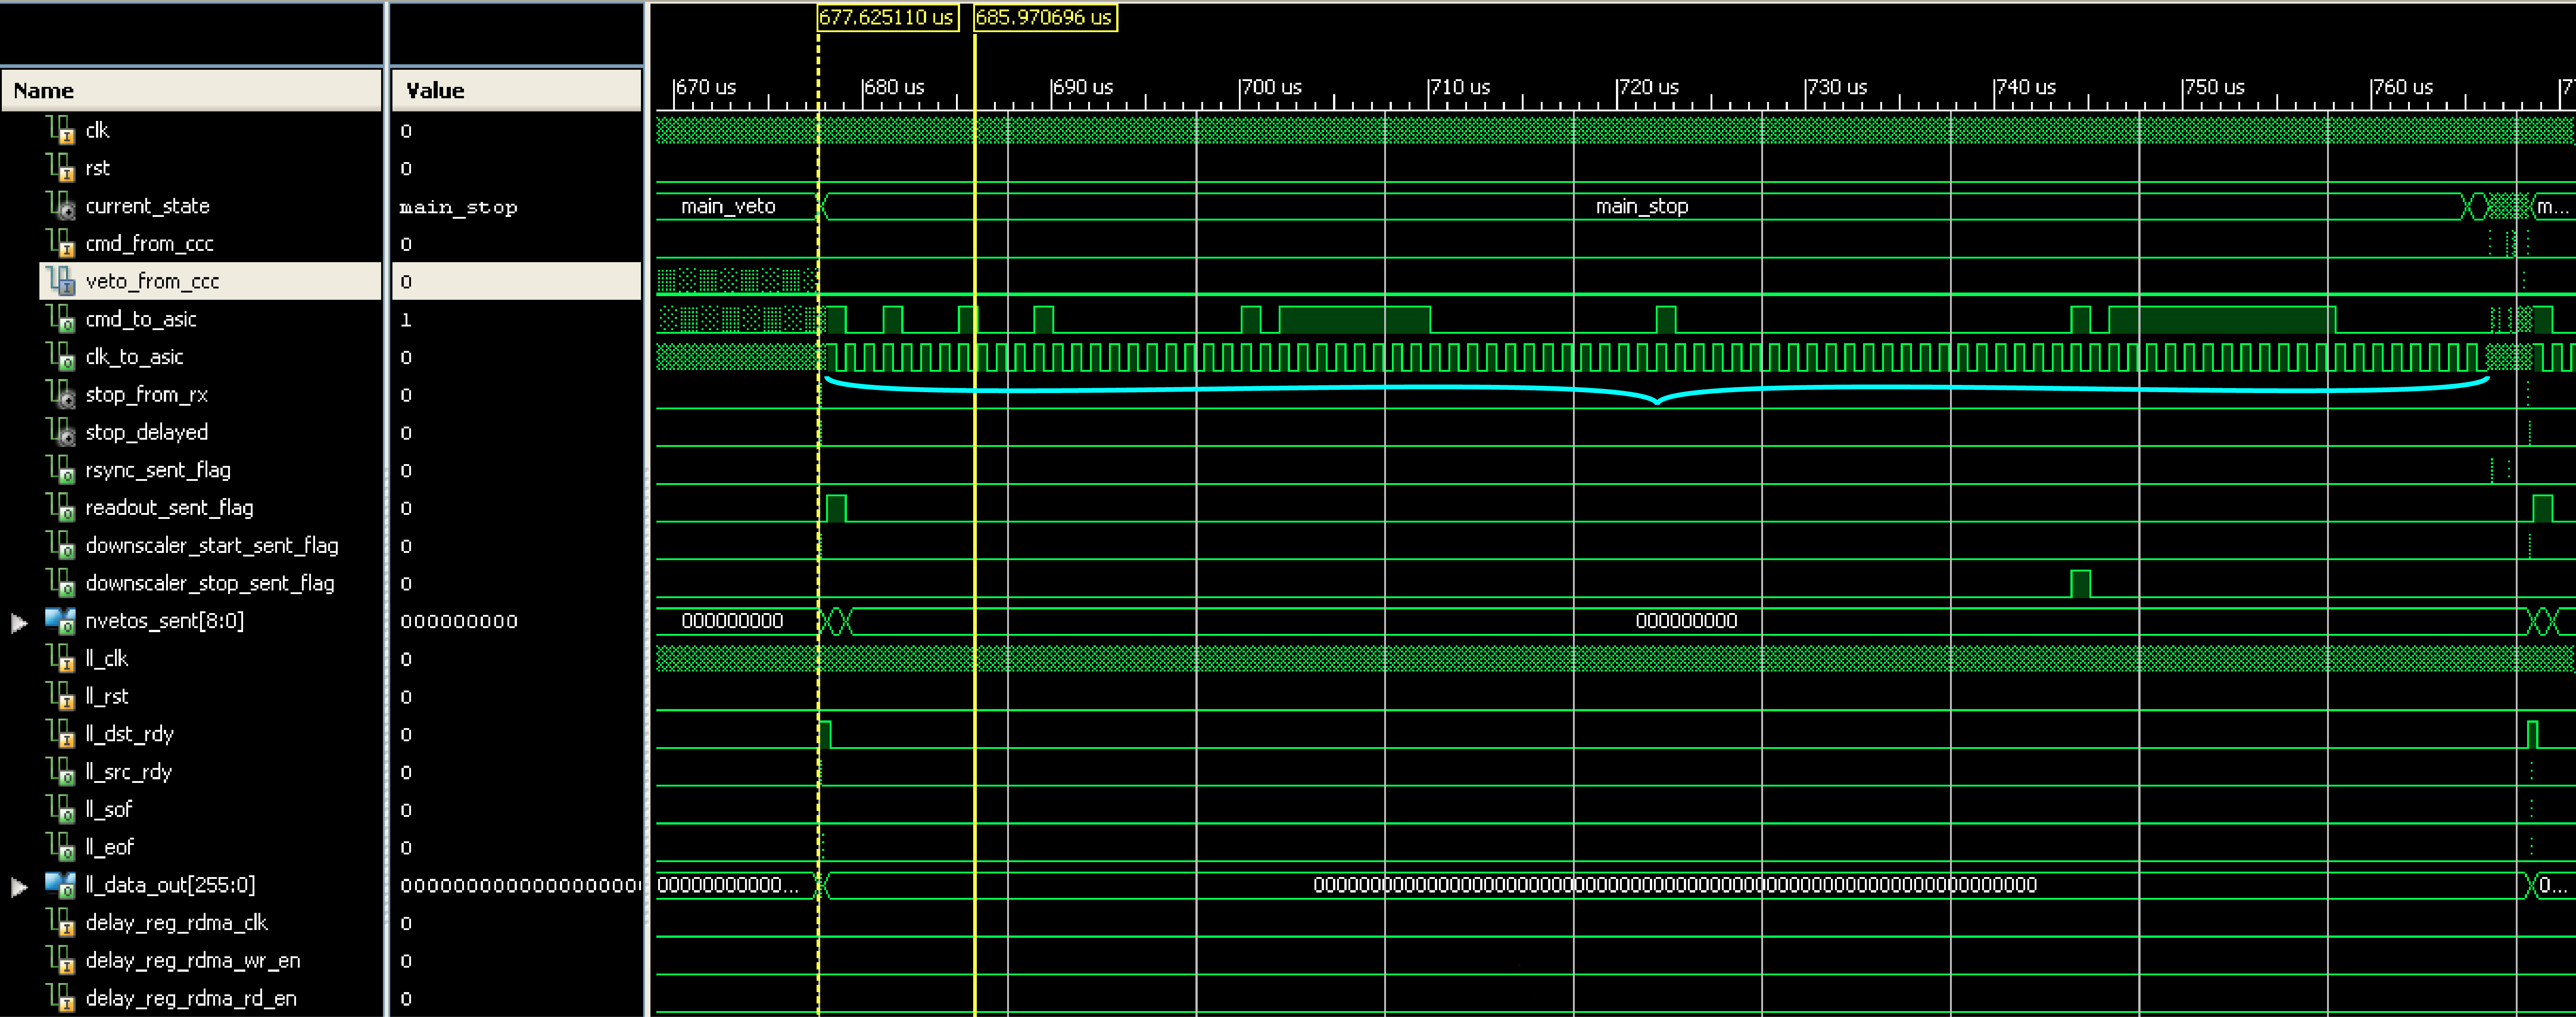
\includegraphics[width=\textwidth]{images/isim/edited/stop-downscaler.png}
  \caption{The \texttt{clk\_to\_asic} down-scaled by a factor of 100. The section delimitated by the yellow guides is shown in figure~\ref{fig:isim_stop-downscaler-zoom}. Note that the second word sent (after the down-scaler trigger) is the \texttt{READ\_OUT\_START} command, the flag is also down-scaled.}
  \label{fig:isim_stop-downscaler}
\end{sidewaysfigure}
    
\begin{sidewaysfigure}[H]
  \centering  
  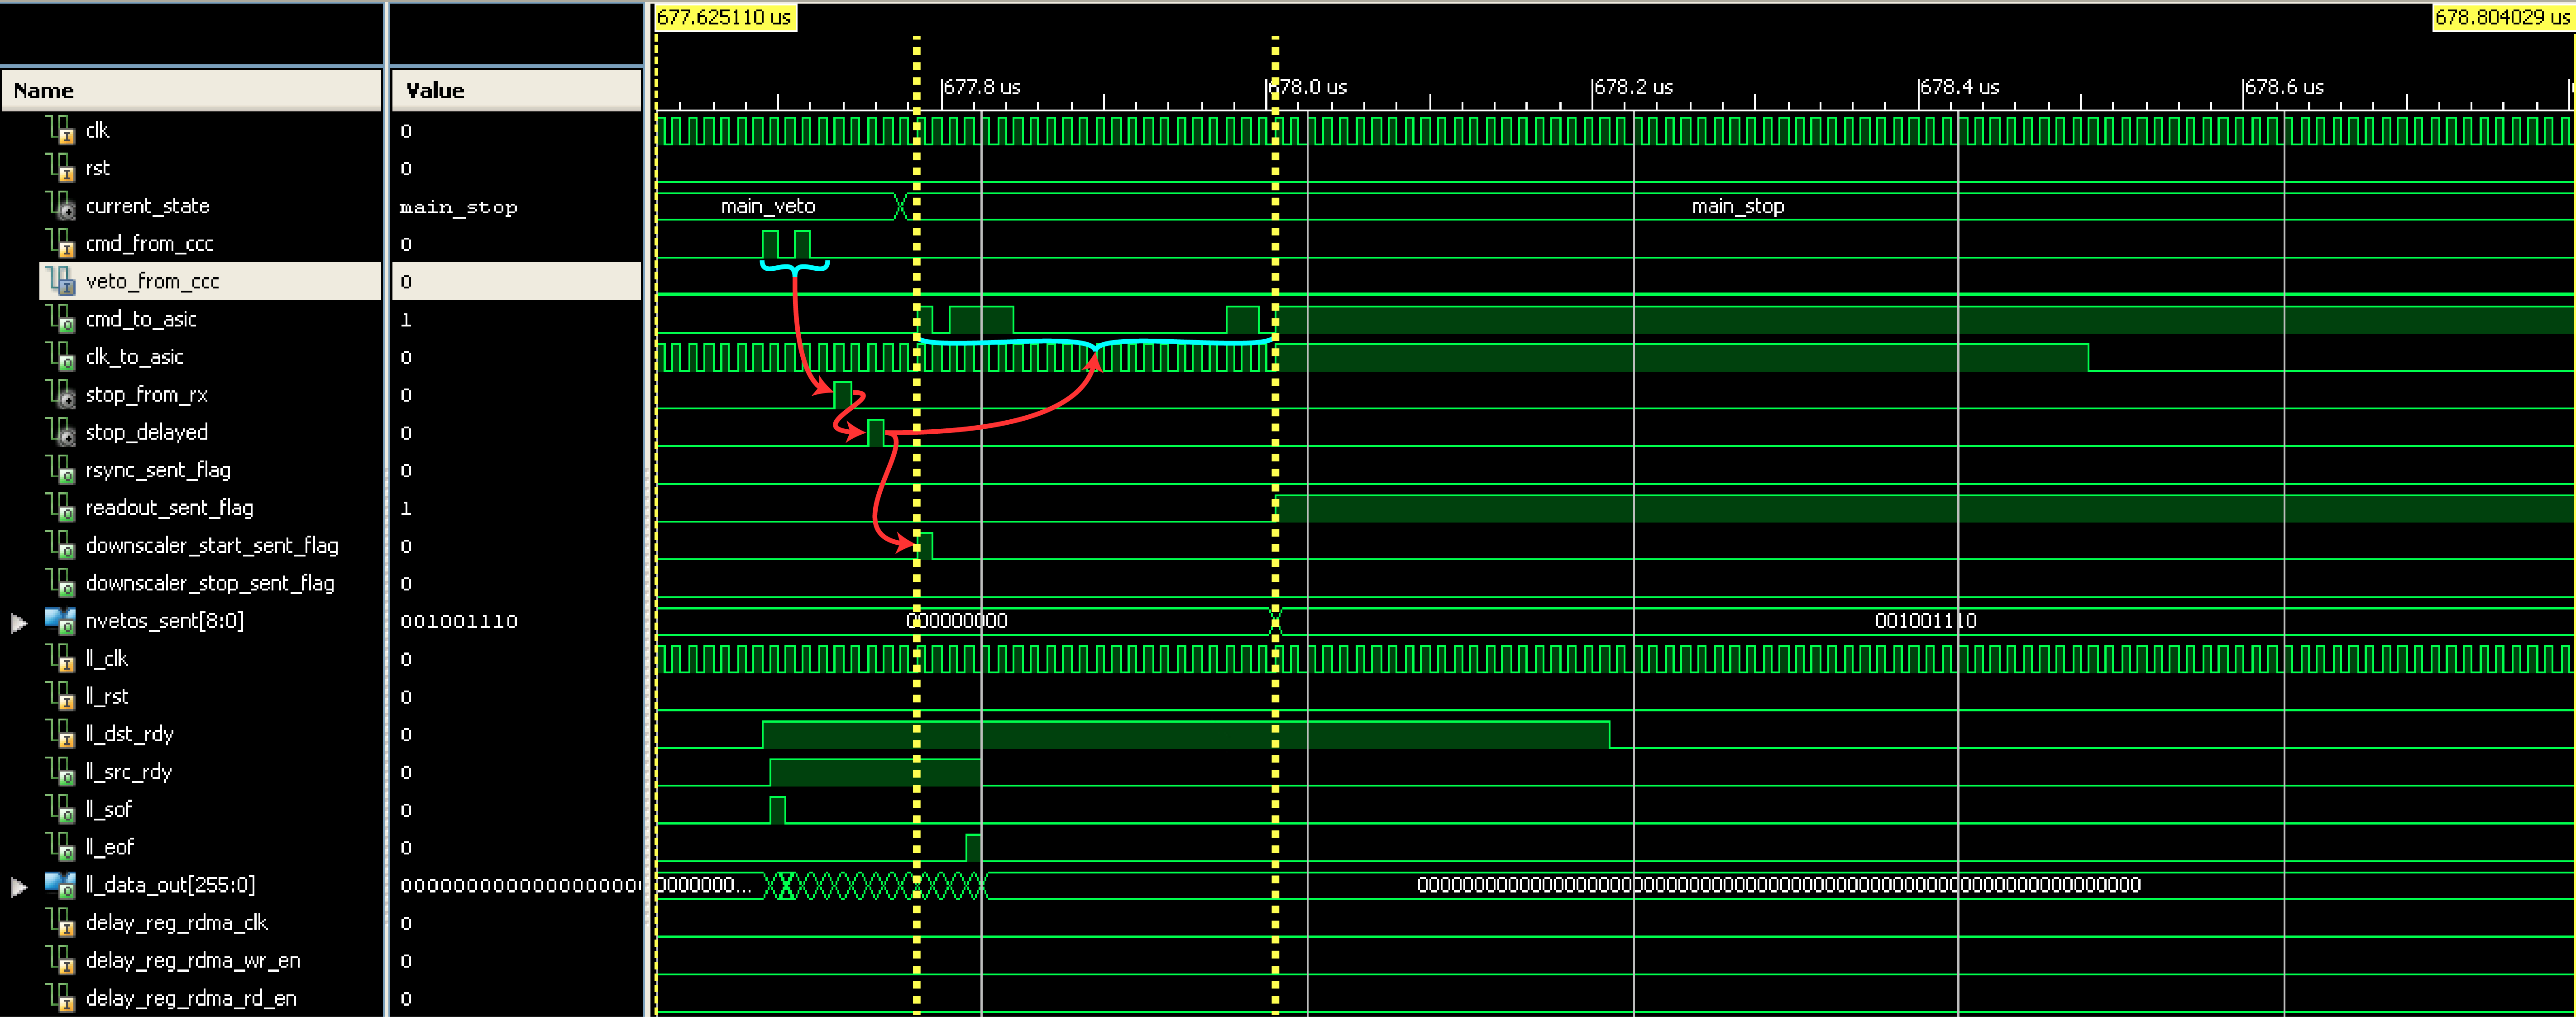
\includegraphics[width=\textwidth]{images/isim/edited/stop-downscaler-zoom.png}
  \caption{The \texttt{STOP} command and down-scaler start word being sent. Note the LocalLink transfer on the `ll\_' lines.}
  \label{fig:isim_stop-downscaler-zoom}
\end{sidewaysfigure}
% subsection stop_downscaler (end)
\clearpage
\subsection{RDMA} % (fold)
\label{sec:rdma}
Figure~\ref{fig:isim_rdma} shows a simple test of the RDMA accessible registers and BRAMs. The first four addresses of each entity is read out. These were checked by hand against the values written at the start.
\begin{sidewaysfigure}[H]
  \centering
  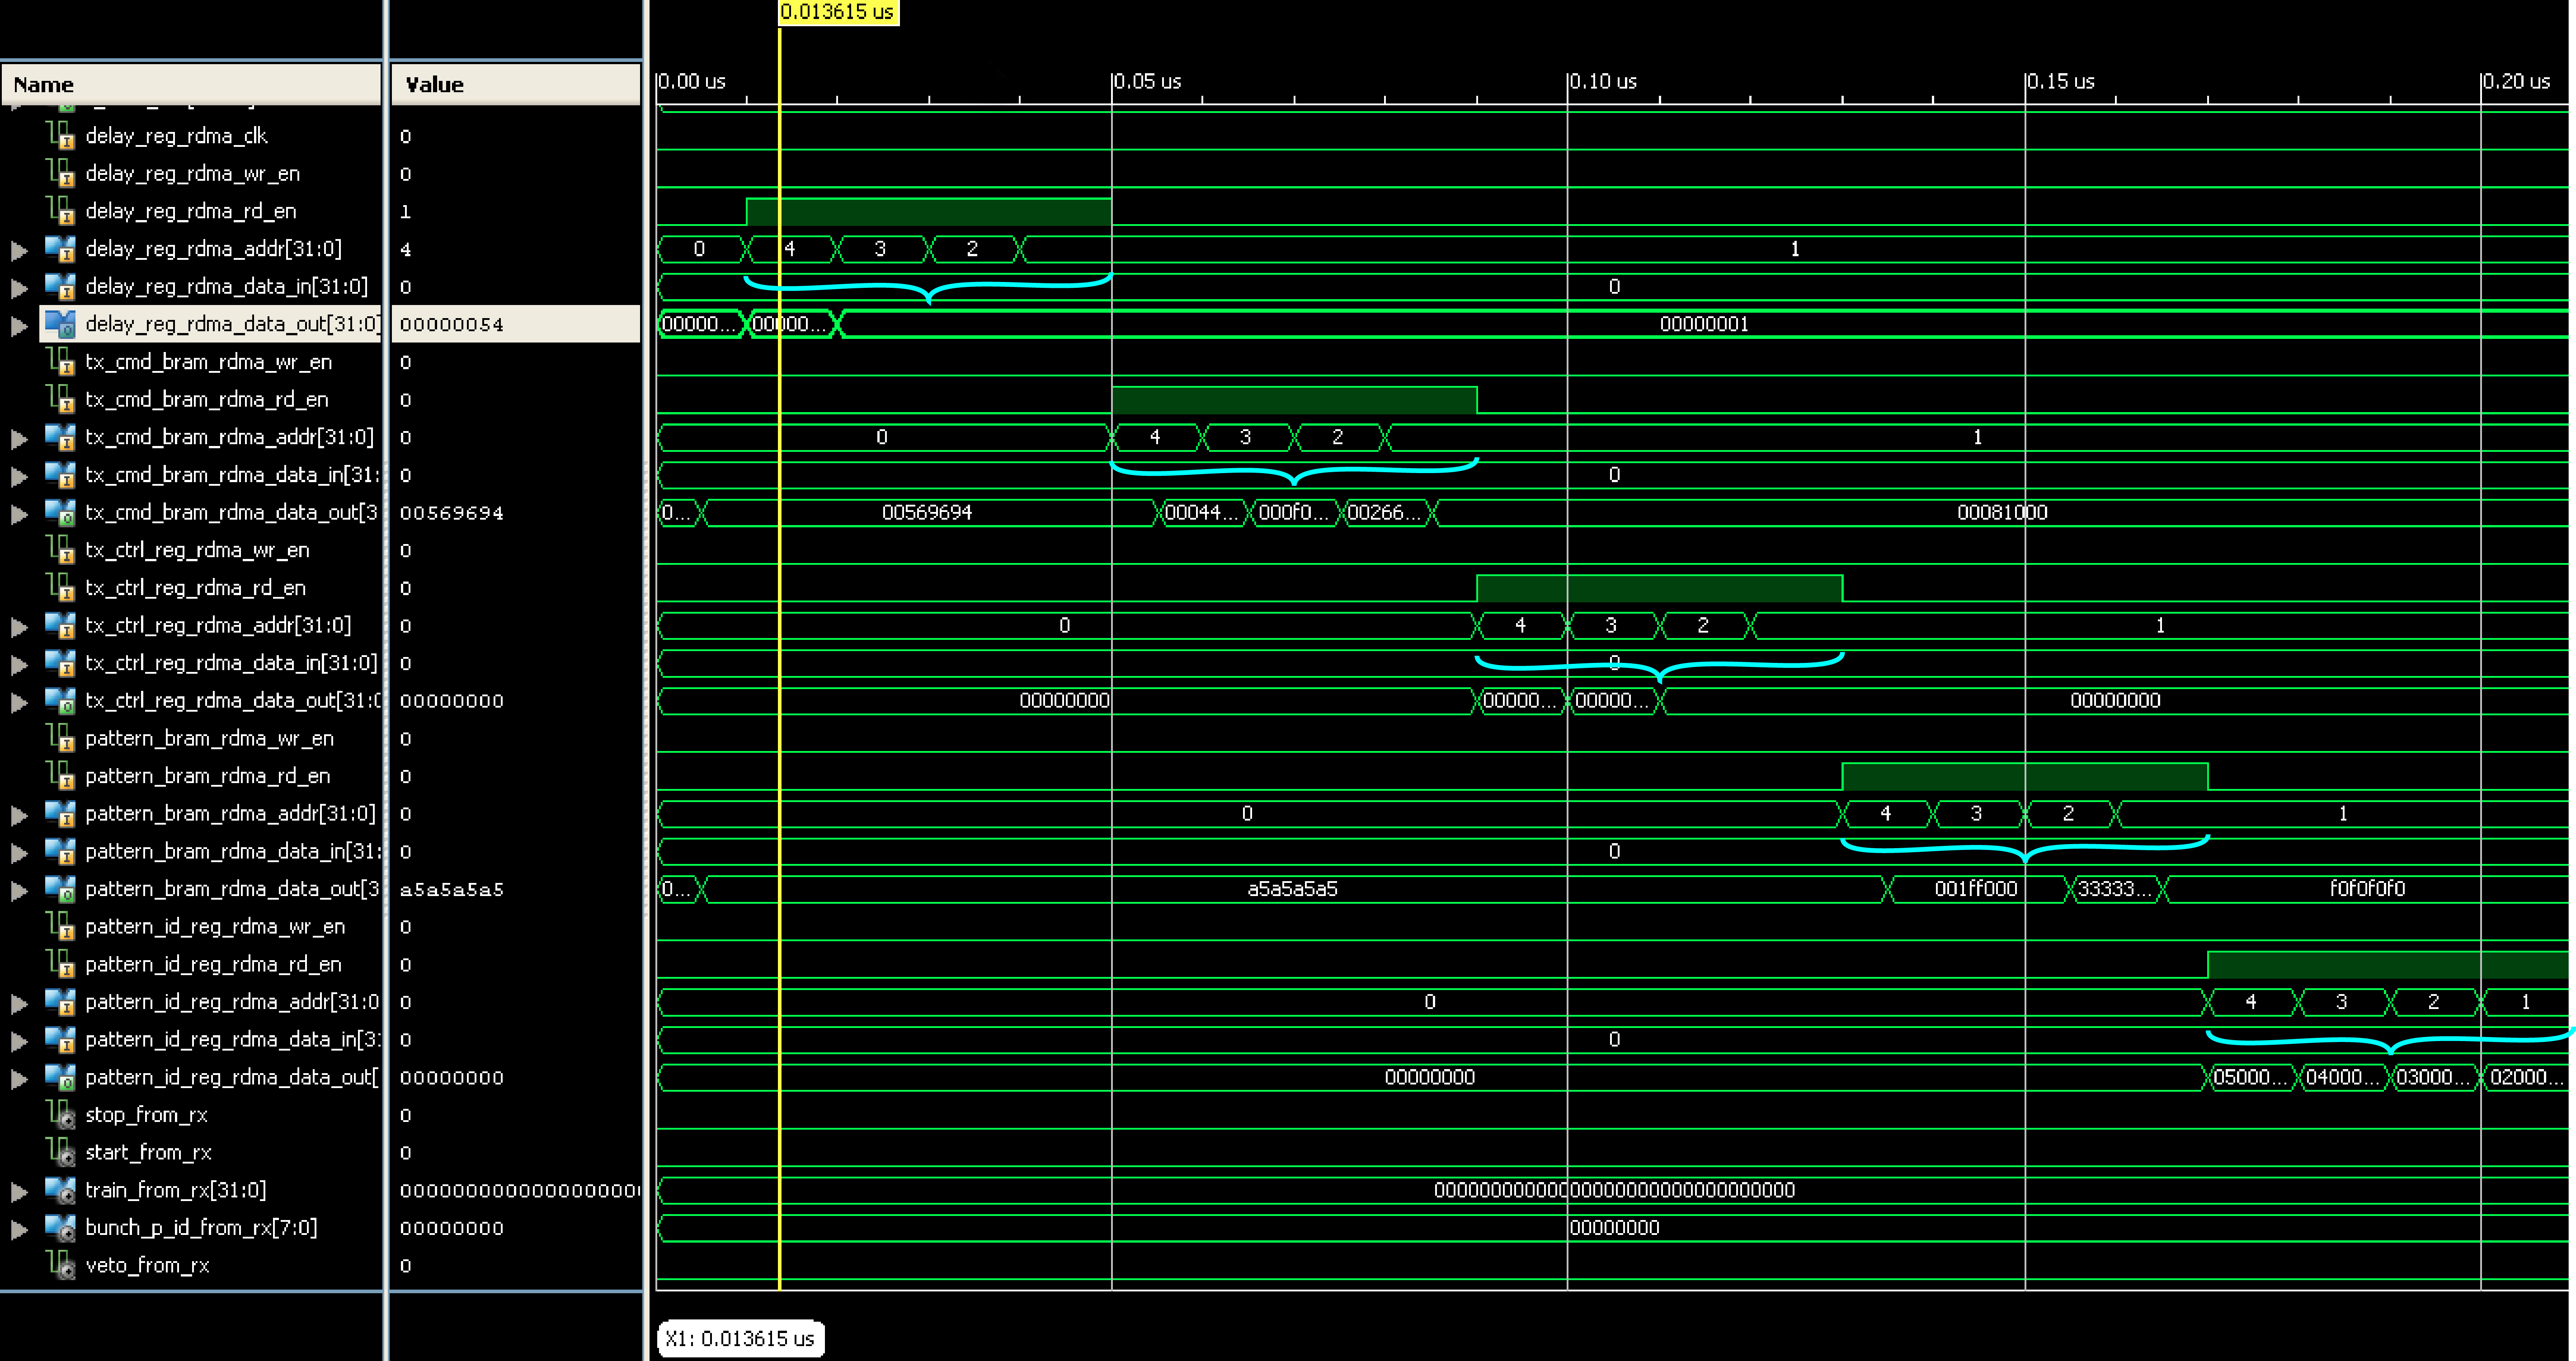
\includegraphics[width=\textwidth]{images/isim/edited/rdma.png}
  \caption{Read back of the first 4 locations of every entity accessible via RDMA.}
  \label{fig:isim_rdma}
\end{sidewaysfigure}
    
% subsection rdma (end)
\clearpage
\subsection{Local Link} % (fold)
\label{sec:local_link}
A sample read-out of the veto-log is shown in figure~\ref{fig:isim_locallink}. The LocalLink specification requires that data transfer starts as soon as both source and destination are read. In this test all bunches were vetoed apart from the first \(n\) of each 256 bunches (where \( n\) is the \( n^{th} \) block of 256 bunches), this resulted in the top bits being filled with 0's; the first word is 0-padded and contains the header information (i.e.\ the train ID and the bunch pattern ID).
\begin{sidewaysfigure}[H]
  \centering
  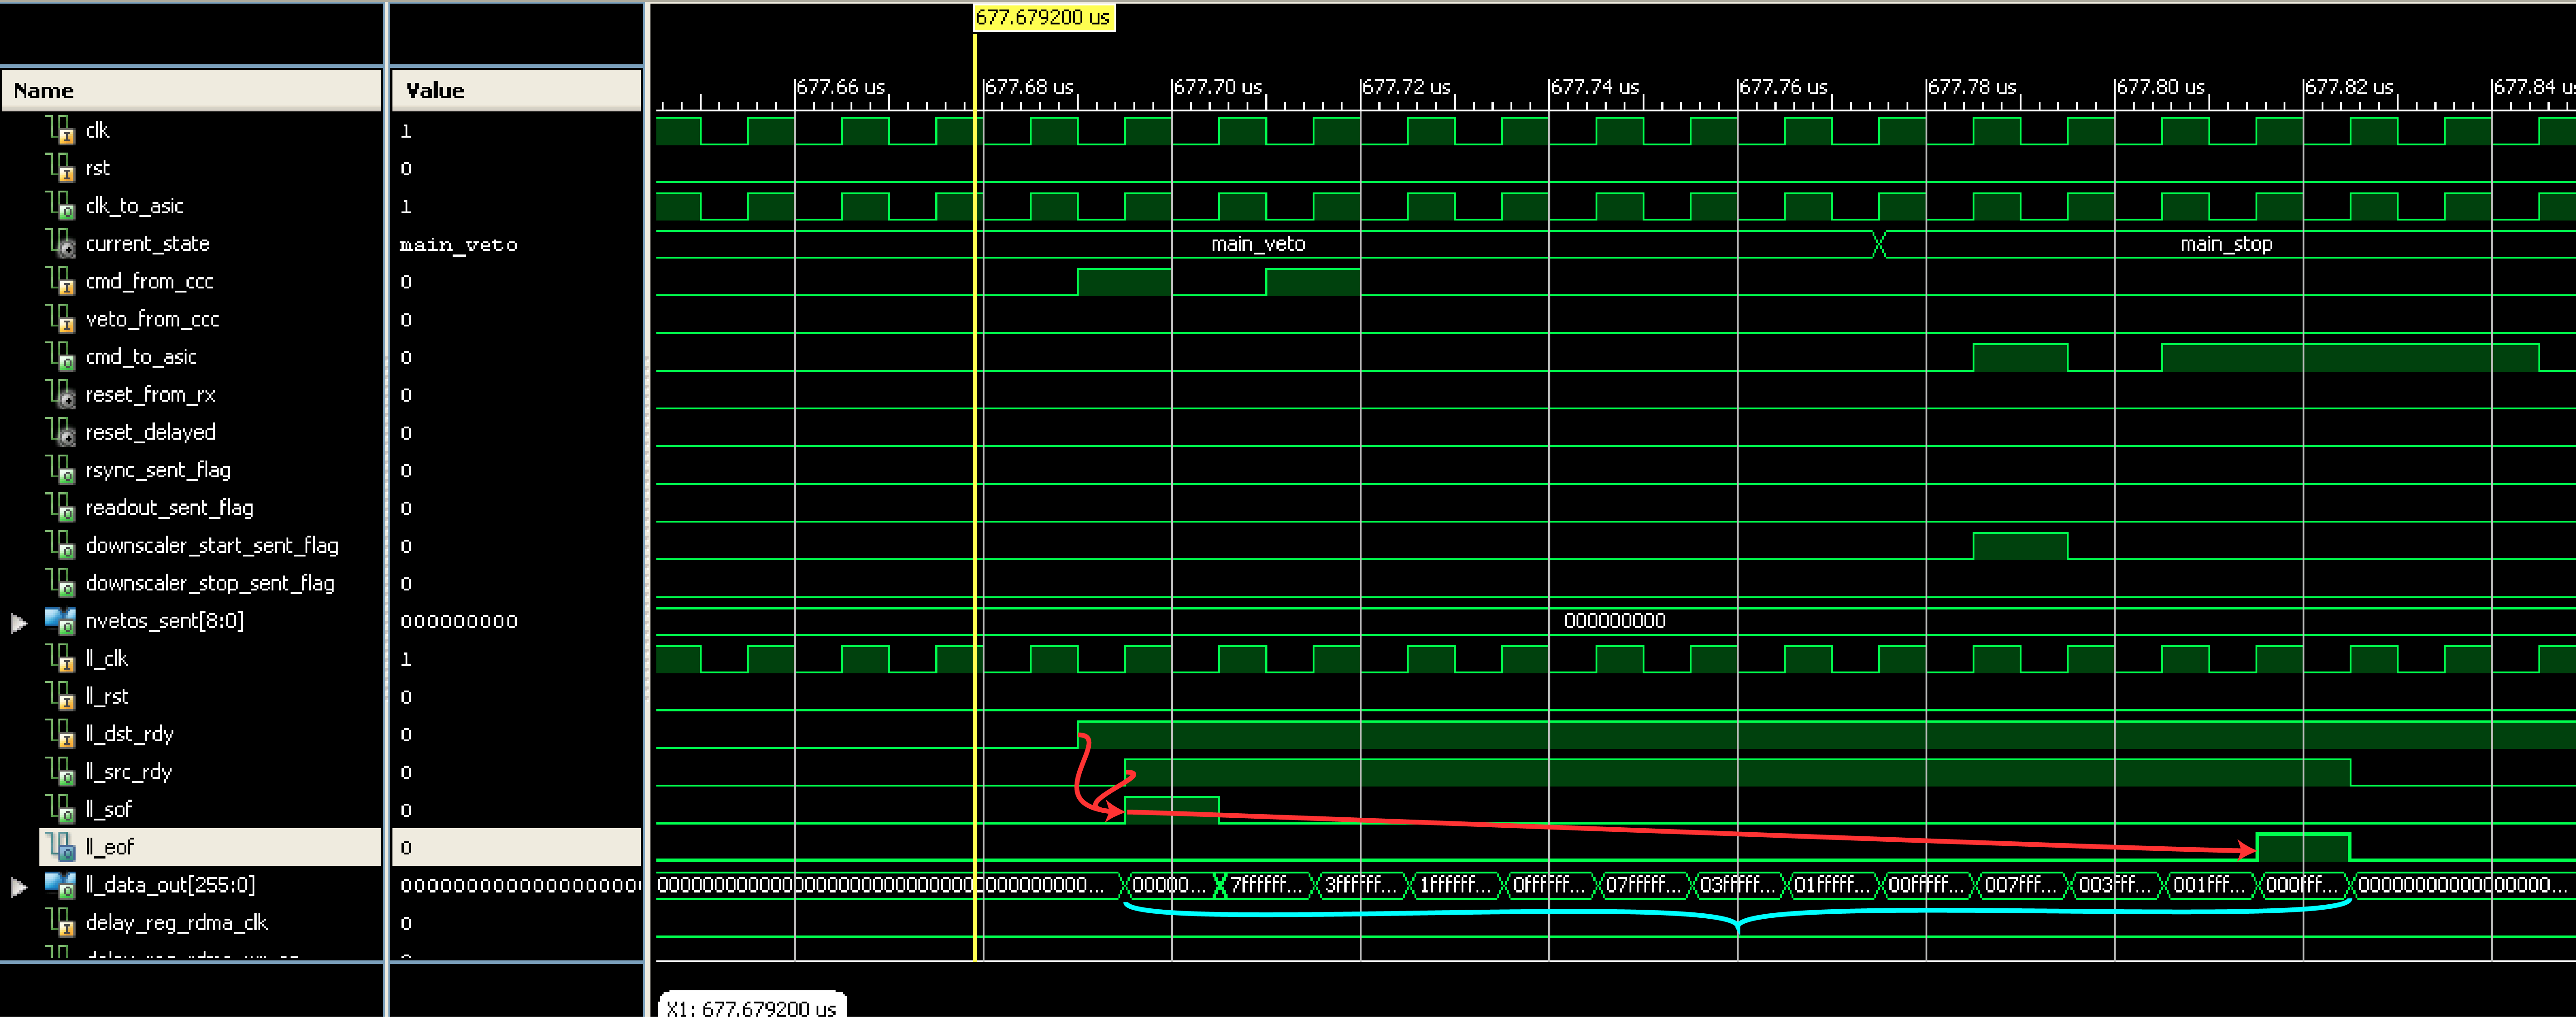
\includegraphics[width=\textwidth]{images/isim/edited/locallink.png}
  \caption{Read-out of the veto log for 3072 bunches.}
  \label{fig:isim_locallink}
\end{sidewaysfigure}
    
% subsection local_link (end)
\clearpage
% section results (end)
%%%%%%%%%%%%%%%%%%%%%%%%%%%%%%%%%%%%%%%%%%%%%%%%%%%
% chapter timing_diagrams (end)
%%%%%%%%%%%%%%%%%%%%%%%%%%%%%%%%%%%%%%%%%%%%%%%%%%%
\chapter{Conclusion} % (fold)
\label{cha:conclusion}
EuXFEL is a huge project, 3.4~km of systems and sub-systems that must be kept in sync at all times in order to work. One of these many sub-systems is the LPD, one of three planned 2D pixel detectors, that will record up to 5,120\( \times \)1~Mpixel images every second. Control of this detector is achieved via 16 FEMs each of which uses a command signal and clock signal, distributed to its supermodule of 512 ASICs, to maintain order. To provide a simple interface between the 2D detectors and the rest of EuXFEL the CCC uses three lines to distribute a \( \sim \)99~MHz clock, a fast command signal, and a veto signal whilst receiving status information. 

The LPD-CCC interface firmware runs on the FEM and provides translation from the three received signals to the two that each ASIC expects. This interface was split into three entities that dealt with receiving, vetoing and transmitting the information from the CCC. Using a rigorous testing regime each entity was developed according to the requirements of both LPD and CCC. The final designs use a combination of state-machines and BRAM to respond rapidly and accurately to each in-bound signal.

Whilst EuXFEL is several years off of operation the interface is already proving its mettle having been used in a recent beam test of the LPD detector at LCLS and in test benches for the CCC board itself.

% chapter conclusion (end)
%%%%%%%%%%%%%%%%%%%%%%%%%%%%%%%%%%%%%%%%%%%%%%%%%%%
\appendix
\chapter{EuXFEL Appendix} % (fold)
\label{cha:appendix}
\section{ASIC command words} % (fold)
\label{app:asic_command_words}
The table~\ref{tab:asic_command_words} provides a full list of all commands implemented by the LPD ASIC, for discussion of what they do see the LPD manual~\cite{lpd_manual}.

\begin{table} [htbp]
  \begin{center} 
    \setlength{\extrarowheight}{1.5pt}
    \begin{tabular}{c | l || c|l}
      Word & Name &  Word & Name \\
      \hline  
      0x00 & NOP                      &  0x0D    & RESET\_TRIGGER\_POINTER     \\
      0x01 & STAND\_BY                &  0x0E    & START\_WRITE\_POINTER       \\
      0x02 & POWER\_UP                &  0x0F    & START\_TRIGGER\_POINTER     \\
      0x03 & ON\_CHIP\_RESET\_DISABLE &  0x10    & TRIGGER\_FLAG\_SET          \\
      0x04 & ON\_CHIP\_RESET\_ENABLE  &  0x11    & READ\_OUT\_DATA             \\
      0x05 & RESET\_PRE\_AMP          &  0x12    & REMOVE\_RESET\_PRE\_AMP     \\
      0x06 & RESET\_GAIN\_FRONT       &  0x13    & REMOVE\_RESET\_GAIN\_STAGE1 \\
      0x07 & RESET\_GAIN\_BACK        &  0x14    & REMOVE\_RESET\_GAIN\_STAGE2 \\
      0x08 & Reserved                 &  0x15    & CLOCK\_DIV\_SEL             \\
      0x09 & TEST\_MODE\_D            &  0x16    & SELF\_TEST\_EN              \\
      0x0A & TUNE\_MODE               &  0x17    & STOP\_READ\_OUT             \\
      0x0B & CLEAR\_SKIP\_REGISTER    &  0x18    & RESET\_STATE\_MACHINE       \\
      0x0C & RESET\_WRITE\_POINTER    &  0x5A5A5 & SYNC\_RESET                 \\
    \end{tabular}
  \end{center}
  \caption{ASIC command words, see \cite{lpd_manual} for a full description and recommended use of these commands.}
  \label{tab:asic_command_words}
\end{table}
% section asic_command_words (end)
%%%%%%%%%%%%%%%%%%%%%%%%%%%%%%%%%%%%%%%%%%%%%%%%%%%
\section{RDMA interface} % (fold)
\label{app:rdma_interface}
The RDMA interfaces used throughout the project have the interface seen in table~\ref{tab:rdma_interface}. The appropriate mask for the address is given in appropriate interface notes. In general for BRAMs a size of 32\(\times\)1024 the appropriate bits are 9:0 whilst for registers the bits 3:0 are used. 
    
\begin{table}[htbp]
  \begin{center}
    \begin{tabulary}{\textwidth}{l|c|c|L}
      Name & Direction & Type & Notes \\
      \hline
      clk       & \multirow{6}{*}{in}
      & sl                & The RDMA clock (this can be separate from e.g. the CCC clock).\\
      rst       &     & sl                & Reset the memory to some default state.                       \\
      rd\_en    &     & sl                & Enable read operations at the address.                        \\
      wr\_en    &     & sl                & Enable write operations at the address.                       \\
      addr      &     & slv (31:0) & The address the MSB will be masked.                           \\
      data\_in  &     & slv (31:0) & Used for writing and otherwise ignored.                       \\
      \hline
      data\_out & out & slv (31:0) & Data out, only guaranteed for read operations.                \\
        
    \end{tabulary}
  \end{center}
  \caption{Standard RDMA interface.}
  \label{tab:rdma_interface}
\end{table}
% section rdma_interface (end)
%%%%%%%%%%%%%%%%%%%%%%%%%%%%%%%%%%%%%%%%%%%%%%%%%%%
\section{Local Link interface} % (fold)
\label{app:local_link_interface}
The Local Link~\cite{locallink_spec} interface is used only to read out the veto log. The details of the frame composition are given in section~\ref{sec:veto_filter}. The interface used is minimal (i.e. no optional features are used) and given in table~\ref{tab:local_link_interface}.
\begin{table}[htbp]
  \begin{center}
    \begin{tabulary}{\textwidth}{l | c | c | L}
      Name & Direction & Type & Notes \\
      \hline
      clk        & \multirow{3}{*}{in} 
      & sl                 & The LL clock (this can be separate from e.g. the CCC clock).\\
      rst        &     & sl                 & Abort.                                                      \\
      dst\_rdy   &     & sl                 & Destination ready.                                          \\
      \hline
      src\_rdy   & \multirow{4}{*}{out}
      & sl                 & Source ready i.e. this entity.                               \\
      sof        &     & sl                 & Start of frame flag.                                        \\
      eof        &     & sl                 & End of frame flag.                                          \\
      data\_out  &     & slv (255:0) & Data out.                                                   \\
    \end{tabulary}
  \end{center}
  \caption{Minimal local link interface as used by the veto logger.}
  \label{tab:local_link_interface}
\end{table}
  
% section local_link_interface (end)
%%%%%%%%%%%%%%%%%%%%%%%%%%%%%%%%%%%%%%%%%%%%%%%%%%%
  
% chapter appendix (end)

    \bibliographystyle{plain}
    \bibliography{thesis_bib}
\end{document}
    
